\chapter{Used Data and Results}

\section{Freddie Mac's Single Family Loan-Level Dataset}

Freddie Mac, officially known as the Federal Home Loan Mortgage Corporation, is a government-sponsored enterprise (GSE) in the United states and plays a crucial role in the secondary mortgage market. In the primary market, individual customers secure mortgage loans from retail banks. Within the secondary mortgage market, the lender have the option to sell these mortgages to entities like government-sponsored enterprises, e.g. Freddie Mac. This practice provides liquidity to the primary market, subsequently making additional loans available to other customers. GSEs aggregate multiple mortgages into mortgage-backed securities (MBS), which are then sold to various investors, such as insurance companies and hedge funds. \cite{FreddieMac:2023} \cite{SecMortMark:2023}

The Single Family Loan-Level Dataset encompasses a broad range of variables and some of the essential features of this dataset include:

\begin{enumerate}
\item Customer Information: This category includes borrower details such as Credit Score provided by FICO, first-time homebuyer status, occupancy status and number of borrowers.
\item Financial Attributes: The dataset provides important financial indicators such as the (combined) loan-to-value ratio (CLTV, LTV) and debt-to-income ratio (DTI).
\item Loan and Property Details: It also includes information about the properties associated with the loans, such as mortgage insurance percentage, number of units, original unpaid balance, original Loan Term, property type and loan purpose.
\item Loan Performance: This section captures essential data related to historical loan performance. It includes details on delinquency status, zero balance reason codes, modification information and the current deferred unpaid balance.
\item Expenses and Loss Information: Included in the performance data are financial details such as mortgage insurance recoveries, net sale proceeds, legal costs, and actual loss, among others.
\end{enumerate}

\subsection{Data Quality, Limitations and Usage}

Over the years, Freddie Mac has accumulated vast amounts of mortgage loan data. At the direction of the Federal Housing Finance Agency (FHFA), this data has been made publicly available to enhance transparency and assist investors in analyzing credit performance. Freddie Mac's Single Family Loan-Level Dataset is publicly available on their website, where users are required to register and agree to the dataset's terms of use before accessing the data.\cite{FreddieMacData:2023}

While the Single Family Loan-Level Dataset offers a wealth of information, it is essential to consider its quality and limitations. Freddie Mac explicitly states  that they do not guarantee a complete or error-free data set and that it may contain potential biases.The dataset represents mortgages acquired by Freddie Mac, which may not be fully representative of the entire mortgage market. Furthermore, the dataset is subject to data protection regulations leading to the anonymization or removal of personally identifiable information. The data set is updated on a quarterly basis and thus, contain corrections or updates that may impact the analysis.\cite{FreddieMacUG:2023}



\section{Dataset}

The Freddie Mac Dataset consists of the origination and monthly performance data file. The former contains information about the borrower and the mortgage loan collected at the start of the contract. The latter includes monthly snapshots of the mortgage loan's payment, status and loss history. The data preparation and modeling process focuses on the origination data, as the objective is creating an application scoring model. The monthly performance data will be used to approximate a default flag, described in Chapter \ref{sec:aprox_def}. The provided data files cover all months since January 1999 and undergo continuous updates every quarter. On average, each month contains about 157.000 mortgage loans, with the highest number of mortgage loans opened in September 2003 with 577.000 accounts. Table \ref{tab:re_descr} shows the full list of relevant variables, their description and abbreviation:

\begin{longtable}{ Lp{8cm}R }\toprule
\textbf{Variable Name}                             & \textbf{Description}                                                                                                                                                                                                                                                                          & \textbf{Abbr.}       \\\midrule
Credit Score                              & A score from an external source (FICO), indicating the borrower's creditworthiness. The higher the score, the lower the probability of default. Value ranges between 300 and 850 or a value of 9999 will be set.                                                                     & Credit Score       \\\hline
First Time Homebuyer Flag                 & Variable is set to 'Y' if borrower purchased the mortgaged property to use as a primary residence and had no ownership in a different property in preceeding three years before purchase.                                                                                            & Homebuyer Flag     \\\hline
Mortgage Insurance Percentage (MI \%)     & Percentage of loss coverage on the loan, that a mortgage insurer covers after a default. Value ranges between 1\% and 55\% or a value of 999 will be set.                                                                                                                            & MI Perc            \\\hline
Number of Units                           & Number of units in property. Value ranges between 1 and 4 or a value of 99 will be set.                                                                                                                                                                                              & No Units           \\\hline
Occupancy Status                          & Contains values "Primary Residence", "Investment Property", "Second Home", "Not Available"                                                                                                                                                                                           & Occupancy          \\\hline
Original Combined Loan-to-Value (CLTV)    & Ratio: (Original mortgage loan amount + Secondary mortgage loan amount if available) divided by the mortgaged property’s appraised value. Value ranges between 1\% and 998\% or a value of 999 will be set. If the CLTV is lower than CTV, then the value was set to 999.            & CLTV               \\\hline
Original Debt-to-Income (DTI) Ratio       & Ratio: (Monthly debt payments + housing expenses) divided by (monthly income). Value ranges between 0\% and 65\% or a value of 999 will be set.                                                                                                                                      & DTI                \\\hline
Original UPB                              & Unpaid principal balance rounded to the nearest 1.000                                                                                                                                                                                                                                & UPB                \\\hline
Original Loan-to-Value (LTV)              & Ratio: Original mortgage loan amount divided by lesser of the mortgaged property’s appraised value. Value ranges between 1\% and 998\% or a value of 999 will be set.                                                                                                                & LTV                \\\hline
Channel                                   & Contains values "Retail", "Broker", "Correspondent", "TPO Not Specified",  "Not Available"                                                                                                                                                                                           & Channel            \\\hline
Prepayment Penalty Mortgage (PPM) Flag    & Variable is set to 'Y' if borrower is or was obligated to pay a penalty in the event of certain repayments of principal.                                                                                                                                                             & PPM Flag           \\\hline
Amortization Type (Formerly Product Type) & Contains values "Fixed Rate Mortgage",  "Adjustable Rate Mortgage"                                                                                                                                                                                                                   & Amort Type         \\\hline
Property State                            & Two letter statecode of property                                                                                                                                                                                                                                                     & State              \\\hline
Property Type                             & Contains values "Condo", "PUD", "Manufactured Housing", "Single-Family",  "Co-op", "Not Available"                                                                                                                                                                                   & Prop Type          \\\hline
Loan Purpose                              & Contains values "Purchase", "Refinance - Cash Out", "Refinance - No Cash Out", "Not Available"                                                                                                                                                                                       & Loan Purpose       \\\hline
Original Loan Term                        & Number of scheduled monthly payments.                                                                                                                                                                                                                                                & Loan Term          \\\hline
Number of Borrowers                       & Number of borrowers obligated to repay the mortgage. Value ranges between 1 and 10 or a value of 99 will be set.                                                                                                                                                                     & No Borrowers       \\\hline
Super Conforming Flag                     & Variable is set to 'Y' if mortgage loan exceed conforming loan limits.                                                                                                                                                                                                               & Sup Conf Flag      \\\hline
Program Indicator                         & Contains values "Home Possible", "HFA Advantage", "Refi Possible", "Not Available", "Not Applicable"                                                                                                                                                                                 & Prog Flag          \\\hline
HARP Indicator                            & Variable is set to 'Y' if loan is part of Freddie Mac’s Relief Refinance Program                                                                                                                                                                                                     & HARP Flag          \\\hline
Property Valuation Method                 & Contains values "Relief Refinance Loan", "Non-Relief Refinance loan"                                                                                                                                                                                                                 & Prop Val Method    \\\hline
Interest Only (I/O) Indicator             & Variable is set to 'Y' if loan only requires interest payments at the beginning of contract.                                                                                                                                                                                         & Int Only Flag      \\\hline
Current Loan Delinquency Status           & Number of days the borrower is delinquent and calculated under the Mortgage Bankers Association (MBA) method                                                                                                                                                                         & Delinquency Status \\\hline
Zero Balance Code                         & Reason, why the loan's balance was reduced to zero; Contains values "Prepaid or Matured (Voluntary Payoff)", "Third Party Sale", "Short Sale or Charge Off", "Repurchase prior to Property Disposition", "REO Disposition", "Whole Loan sales", "Reperforming sales securitizaitons" & Zero Balance Code 
%\end{tabular}
%\end{table}
\\\bottomrule

\caption{Description of variables}
\label{tab:re_descr}
\end{longtable}

\subsection{Approximation of default flag}
\label{sec:aprox_def}

Since the dataset does not directly contain default information, an approximation for the indicator needs to be created. This information is derived from the performance data of the mortgage loan. As a first step, the number of months between the date of the first payment and the date of being in delinquency continuously for 30/60/90/120/180 days was calculated. To imitate the definition of default described in the CRR 178(1) a (Chapter \ref{sec:dr_pd}) as closely as possible, the 90 days delinquency information was selected for further analysis. Due to data irregularities, where the 120 or 180 DPD field is filled in, but the 90 DPD is missing, the minimum of all three variables was used for the next steps. Additionally, to fulfill the definition of default stated in the CRR 178(1) b, the variable \emph{Zero Balance Code} was incorporated. It contains the reason why the loan balance was reduced to zero, displayed in Table \ref{tab:re_ZB_Descr}. Therefore, Zero Balance Codes 02, 03, 09 and 15 indicate a negative financial health and were considered in the default approximation.


\begin{table}[H]
\centering
\begin{tabular}{ l l }\toprule
\textbf{Zero Balance Code} & \textbf{Description}            \\\midrule
01                & Prepaid or Matured (Voluntary Payoff)    \\
02                & Third Party Sale                         \\
03                & Short Sale or Charge Off                 \\
96                & Repurchase prior to Property Disposition \\
09                & REO Disposition                          \\
15                & Whole Loan sales                         \\
16                & Reperforming sales securitizaitons \\\bottomrule
\end{tabular}%
\caption{Description of Zero Balance Code}
\label{tab:re_ZB_Descr}
\end{table}

In the modeling process, a 12-month time span was chosen. Following the identification of default events, the default flag was set based on the following conditions:

\begin{itemize}
  \item Customer was in delinquency for at least 90 days continuously during the first 12 months in the books.
  \item Loan balance showed a negative behavior in the \emph{Zero Balance Code} during the first 12 months in the books.
\end{itemize}

\section{Sample Creation}

\subsection{Data Exclusions}
The first two months of the whole data set showed an unusually low number of observations and default events, leading to their exclusion. Given the 12-month observation period for the default flag, the final 12 months of the dataset were also omitted. Additionally, accounts that were prepaid before the 12-month observation period ended were removed. Lastly, mortgage loans without monthly performance data were also deleted because it was then impossible to approximate a default flag. The breakdown of exclusions based on each reason is detailed in Table \ref{tab:re_nr_excl}.

\begin{table}[H]
\centering
\begin{tabular}{ l r }\toprule          										
\textbf{Reason}                                       	& \textbf{Number of data entries} 	\\\midrule
Remove first 2 months due to unusual low number 		& 5047                   			\\
Less than 12 months (Last Year)                 		& 2127828                			\\
Less than 12 months and prepaid                 		& 4452984                			\\
Missing Monthly Performance data                		& 1484  				 			\\\bottomrule
\end{tabular}%
\caption{Number of exclusions}
\label{tab:re_nr_excl}
\end{table}

\subsection{Training, Test and Validation Sample}
Figure \ref{fig:re_wholesample} shows the number of observations as well as the default rate per month for the whole sample before and after data exclusions and Figure \ref{fig:re_devsample} is a separate display of the development and out-of-time sample. If the number of defaults had not been sufficient, an increase in the observation window might have been a solution. Both figures show a satisfying number of monthly defaults with an average default rate of 1,52\% in the development sample. A plausible development of the default rate is visible; it follows the expected increase of defaults during the Dot-Com crisis in the late 1990s, the financial crisis in 2007/2008 and the COVID-19 crisis in 2020/2021. 

The development sample encompasses data from January 2018 to December 2020, offering a timeframe that covers different economic conditions, including the period before and during the COVID-19 crisis. This selection not only captures diverse economic scenarios but also limits the number of observations due to the limitation of computational power. The out-of-time sample, referred to as the validation sample, is constructed using data points from January to December 2021.

The data preparation and univariate analysis were performed on the whole development data set, then split into 70\% training and 30\% test samples. The split was stratified on the default flag and the year to ensure a balanced data set for the multivariate analysis and the modeling process of both modeling approaches. Table \ref{tab:re_devoofsample} shows the sample sizes and default rates. Complete lists of the number of accounts and defaults per month for the whole sample before and after exclusion are given in Appendix \ref{sec:DR_whole}.

\begin{table}[H]
\centering
\begin{tabular}{lrrr} \toprule       
\textbf{Sample} & \textbf{\# Accounts} & \textbf{\# Def} & \textbf{\% Def Rate} \\\midrule
Whole Dataset   & 39.404.062           & 208.008         & 0,53\%               \\
Training        & 3.789.579            & 57.510          & 1,52\%               \\
Test            & 1.624.101            & 24.645          & 1,52\%               \\
Out Of Time     & 4.121.718            & 16.848          & 0,41\%               \\\bottomrule
\end{tabular}
\caption{Development and Validation sample}
\label{tab:re_devoofsample}
\end{table}

\begin{figure}[H]
	\centering
	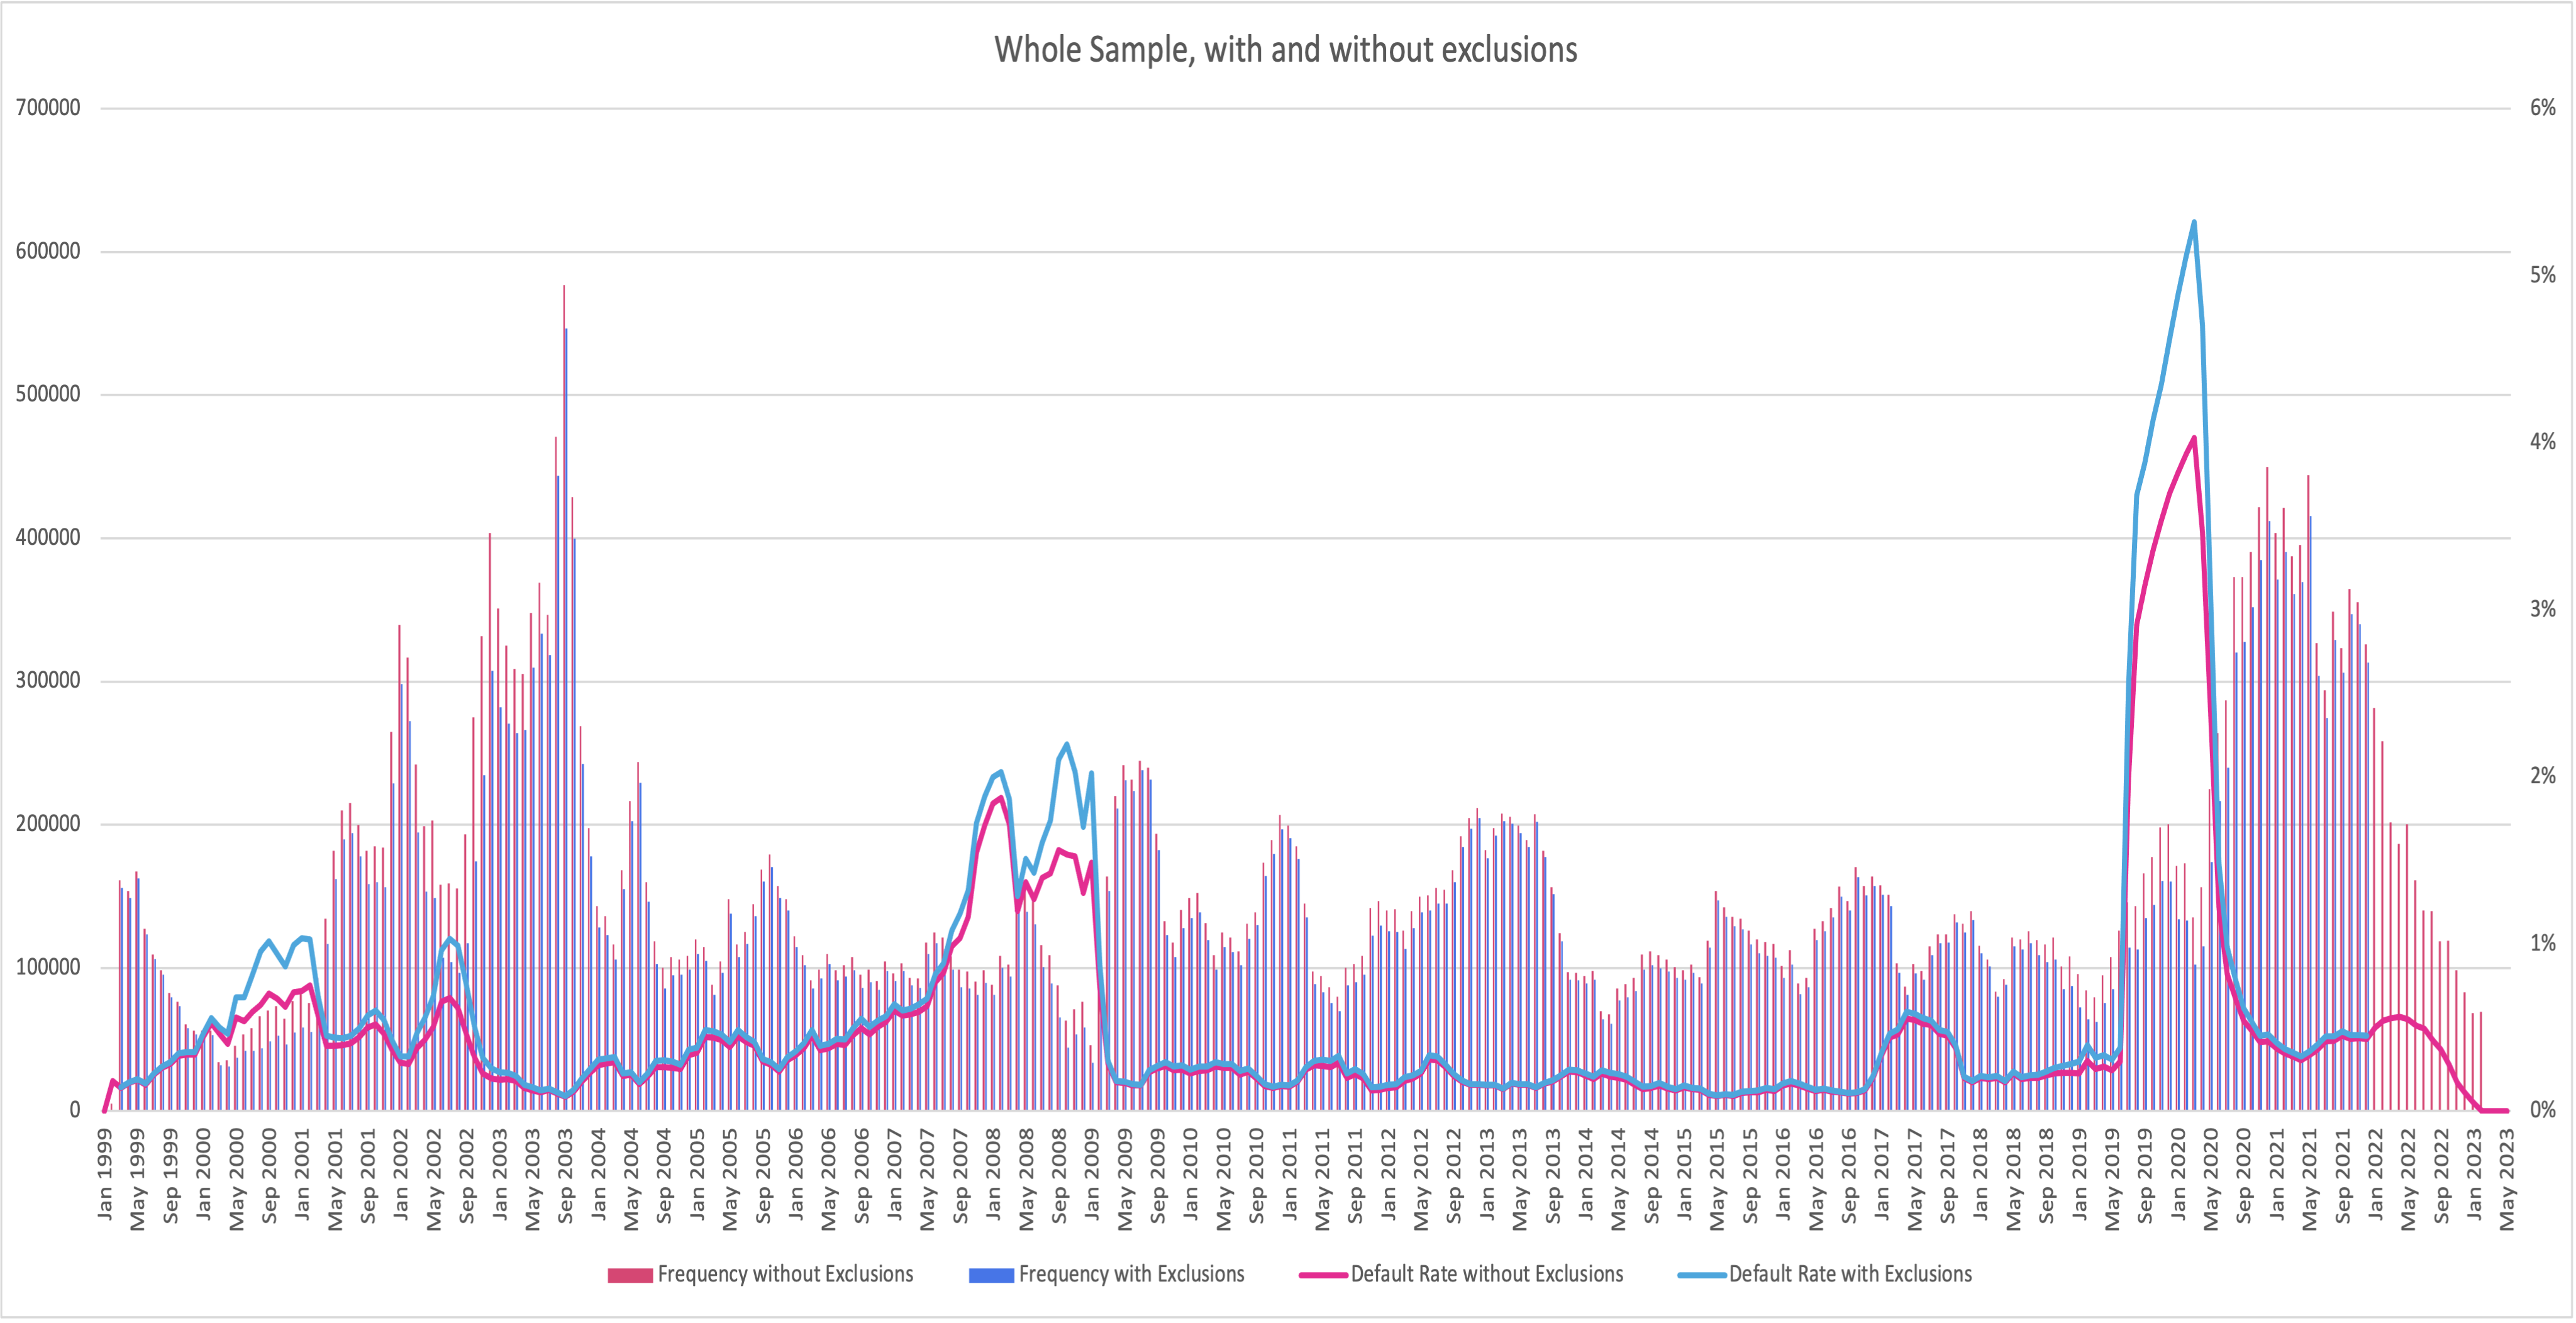
\includegraphics[width=\textwidth]{./FullSample.png}
    \caption{Distribution and default rate of whole sample}
    \label{fig:re_wholesample}
\end{figure}
\begin{figure}[H]
	\centering
	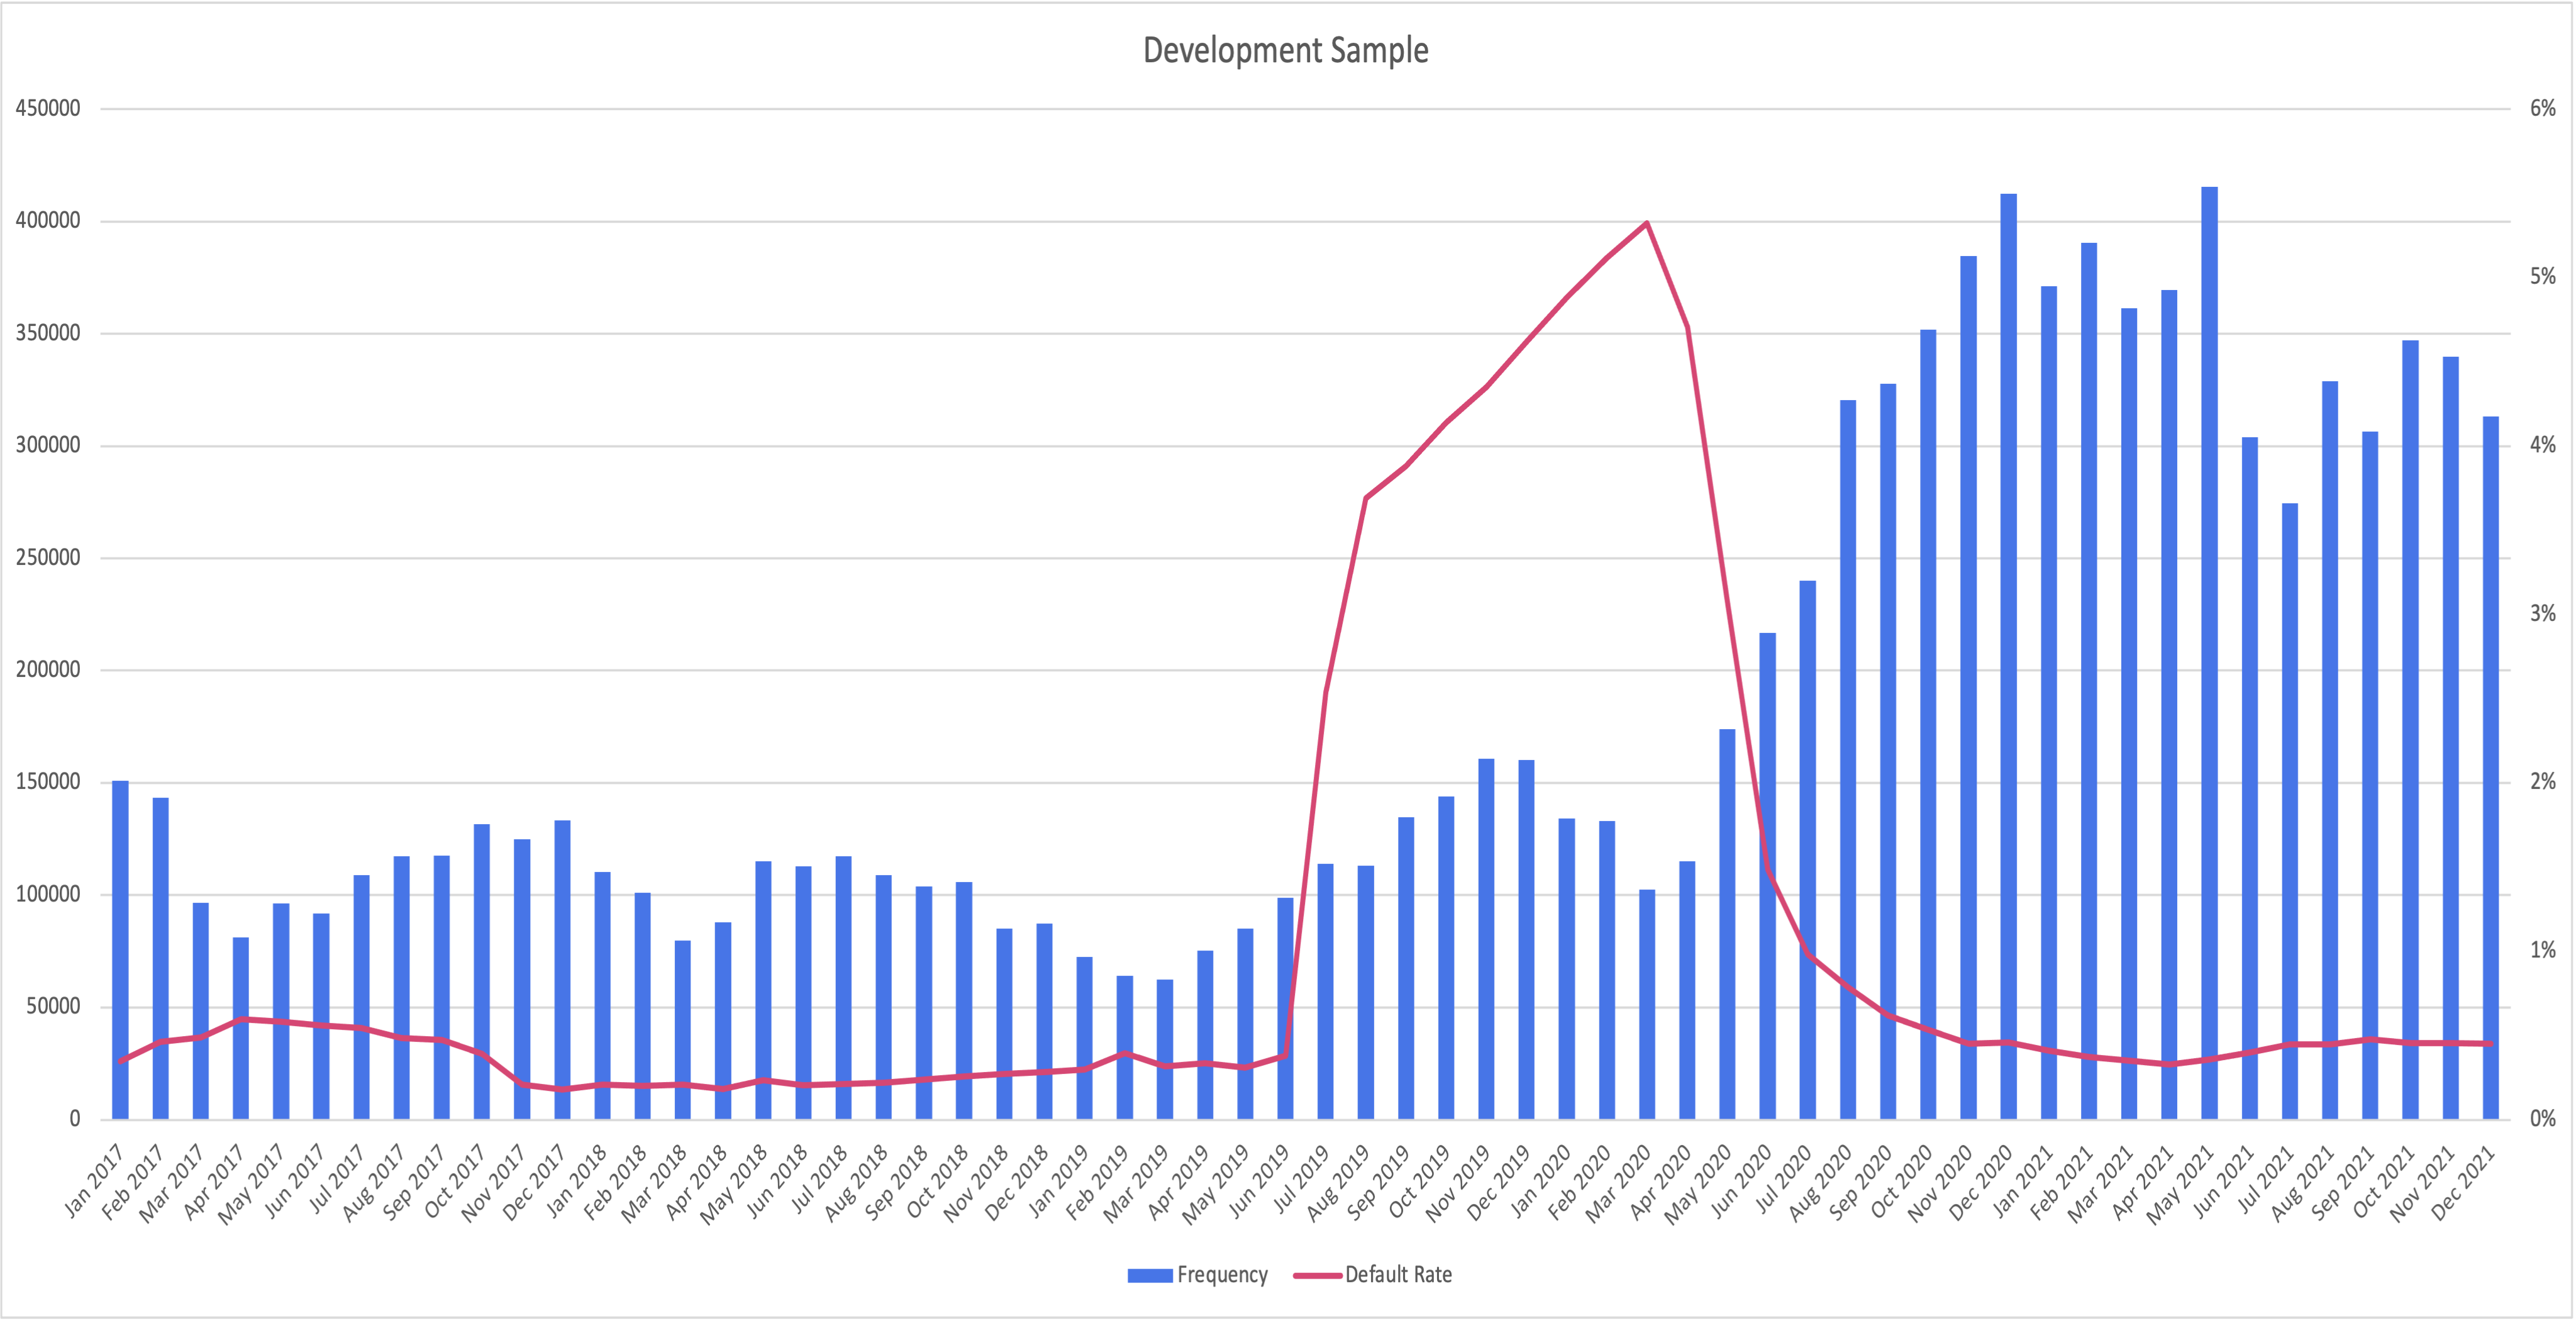
\includegraphics[width=\textwidth]{./DevelopmentSample.png}
    \caption{Distribution and default rate of development and validation sample}
    \label{fig:re_devsample}
\end{figure}

\section{Data preparation}
\subsection{Missing and Erroneous Data Treatment}
The variables were first split into three types: categorical, indicator/binary and numerical variables. The missing rate of all variables were determined and are given in Table \ref{tab:re_discr_power}. \emph{Program Indicator}, \emph{HARP Indicator} and \emph{Super Conforming Flag} exhibit a high proportion of missing values, exceeding 90\%, making them unsuitable for inclusion in the model. On the other hand, all other risk factors either have no missing values or possess an acceptable rate of less than 20\%. Given the low number of missing values for numerical variables such as \emph{DTI} and \emph{Credit Score} and others with a missing rate below the third decimal, imputation was performed using the median, stated in Table \ref{tab:re_descr_stat}. Missing data points for the variable \emph{Property Valuation Method} and other categorical risk factors were treated as a distinct category, while missing values for indicator variables were assigned a value of 'Y'.

No treatment of erroneous data was undertaken, as data entries outside pre-defined ranges were already set as 'Not Available' or '999' by Freddie Mac. Consequently, further analysis for potential errors was deemed unnecessary.
Figure \ref{fig:re_distr1} to \ref{fig:re_distr4} show the distribution plots of relevant risk factors, all plots are given in Appendix \ref{sec:distr_all}.

\begin{figure}[H]
\begin{minipage}{.5\textwidth}
	\centering
	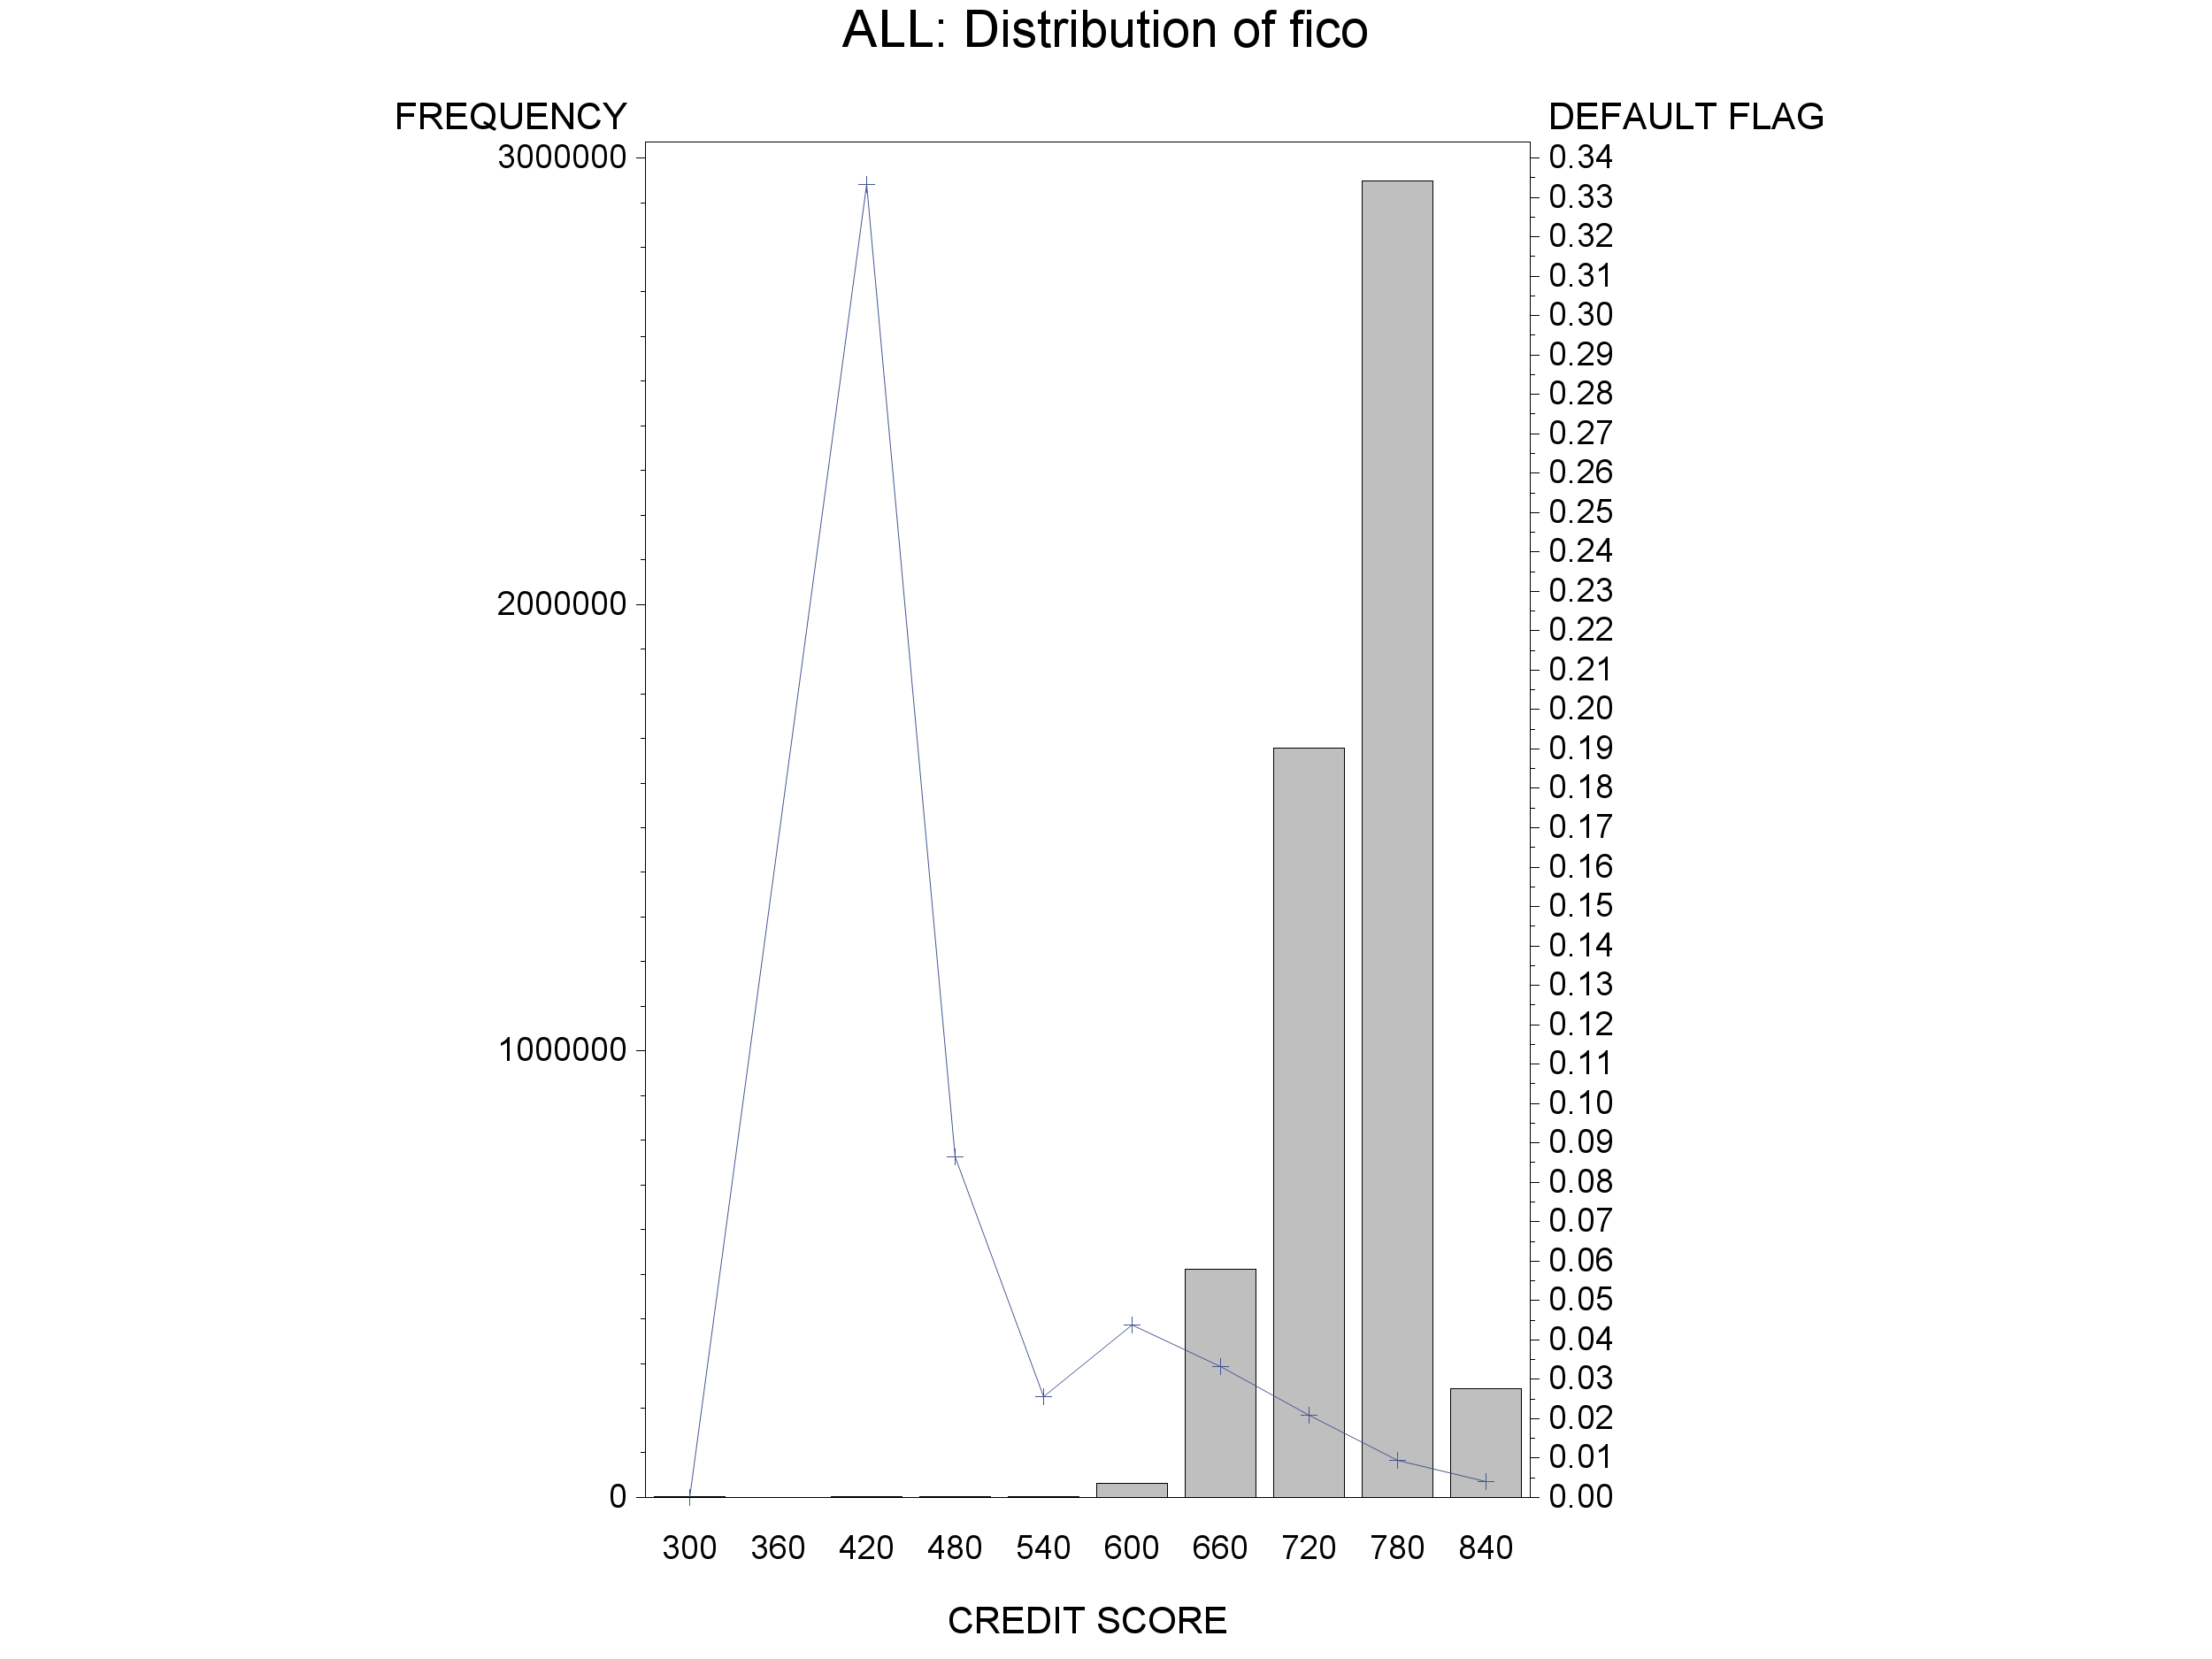
\includegraphics[width=0.9\textwidth]{./plot/Distribution/Main/RE_NUM_fico_DISTRIBUTION_ALL.png}
\end{minipage}%
\begin{minipage}{.5\textwidth}
	\centering
	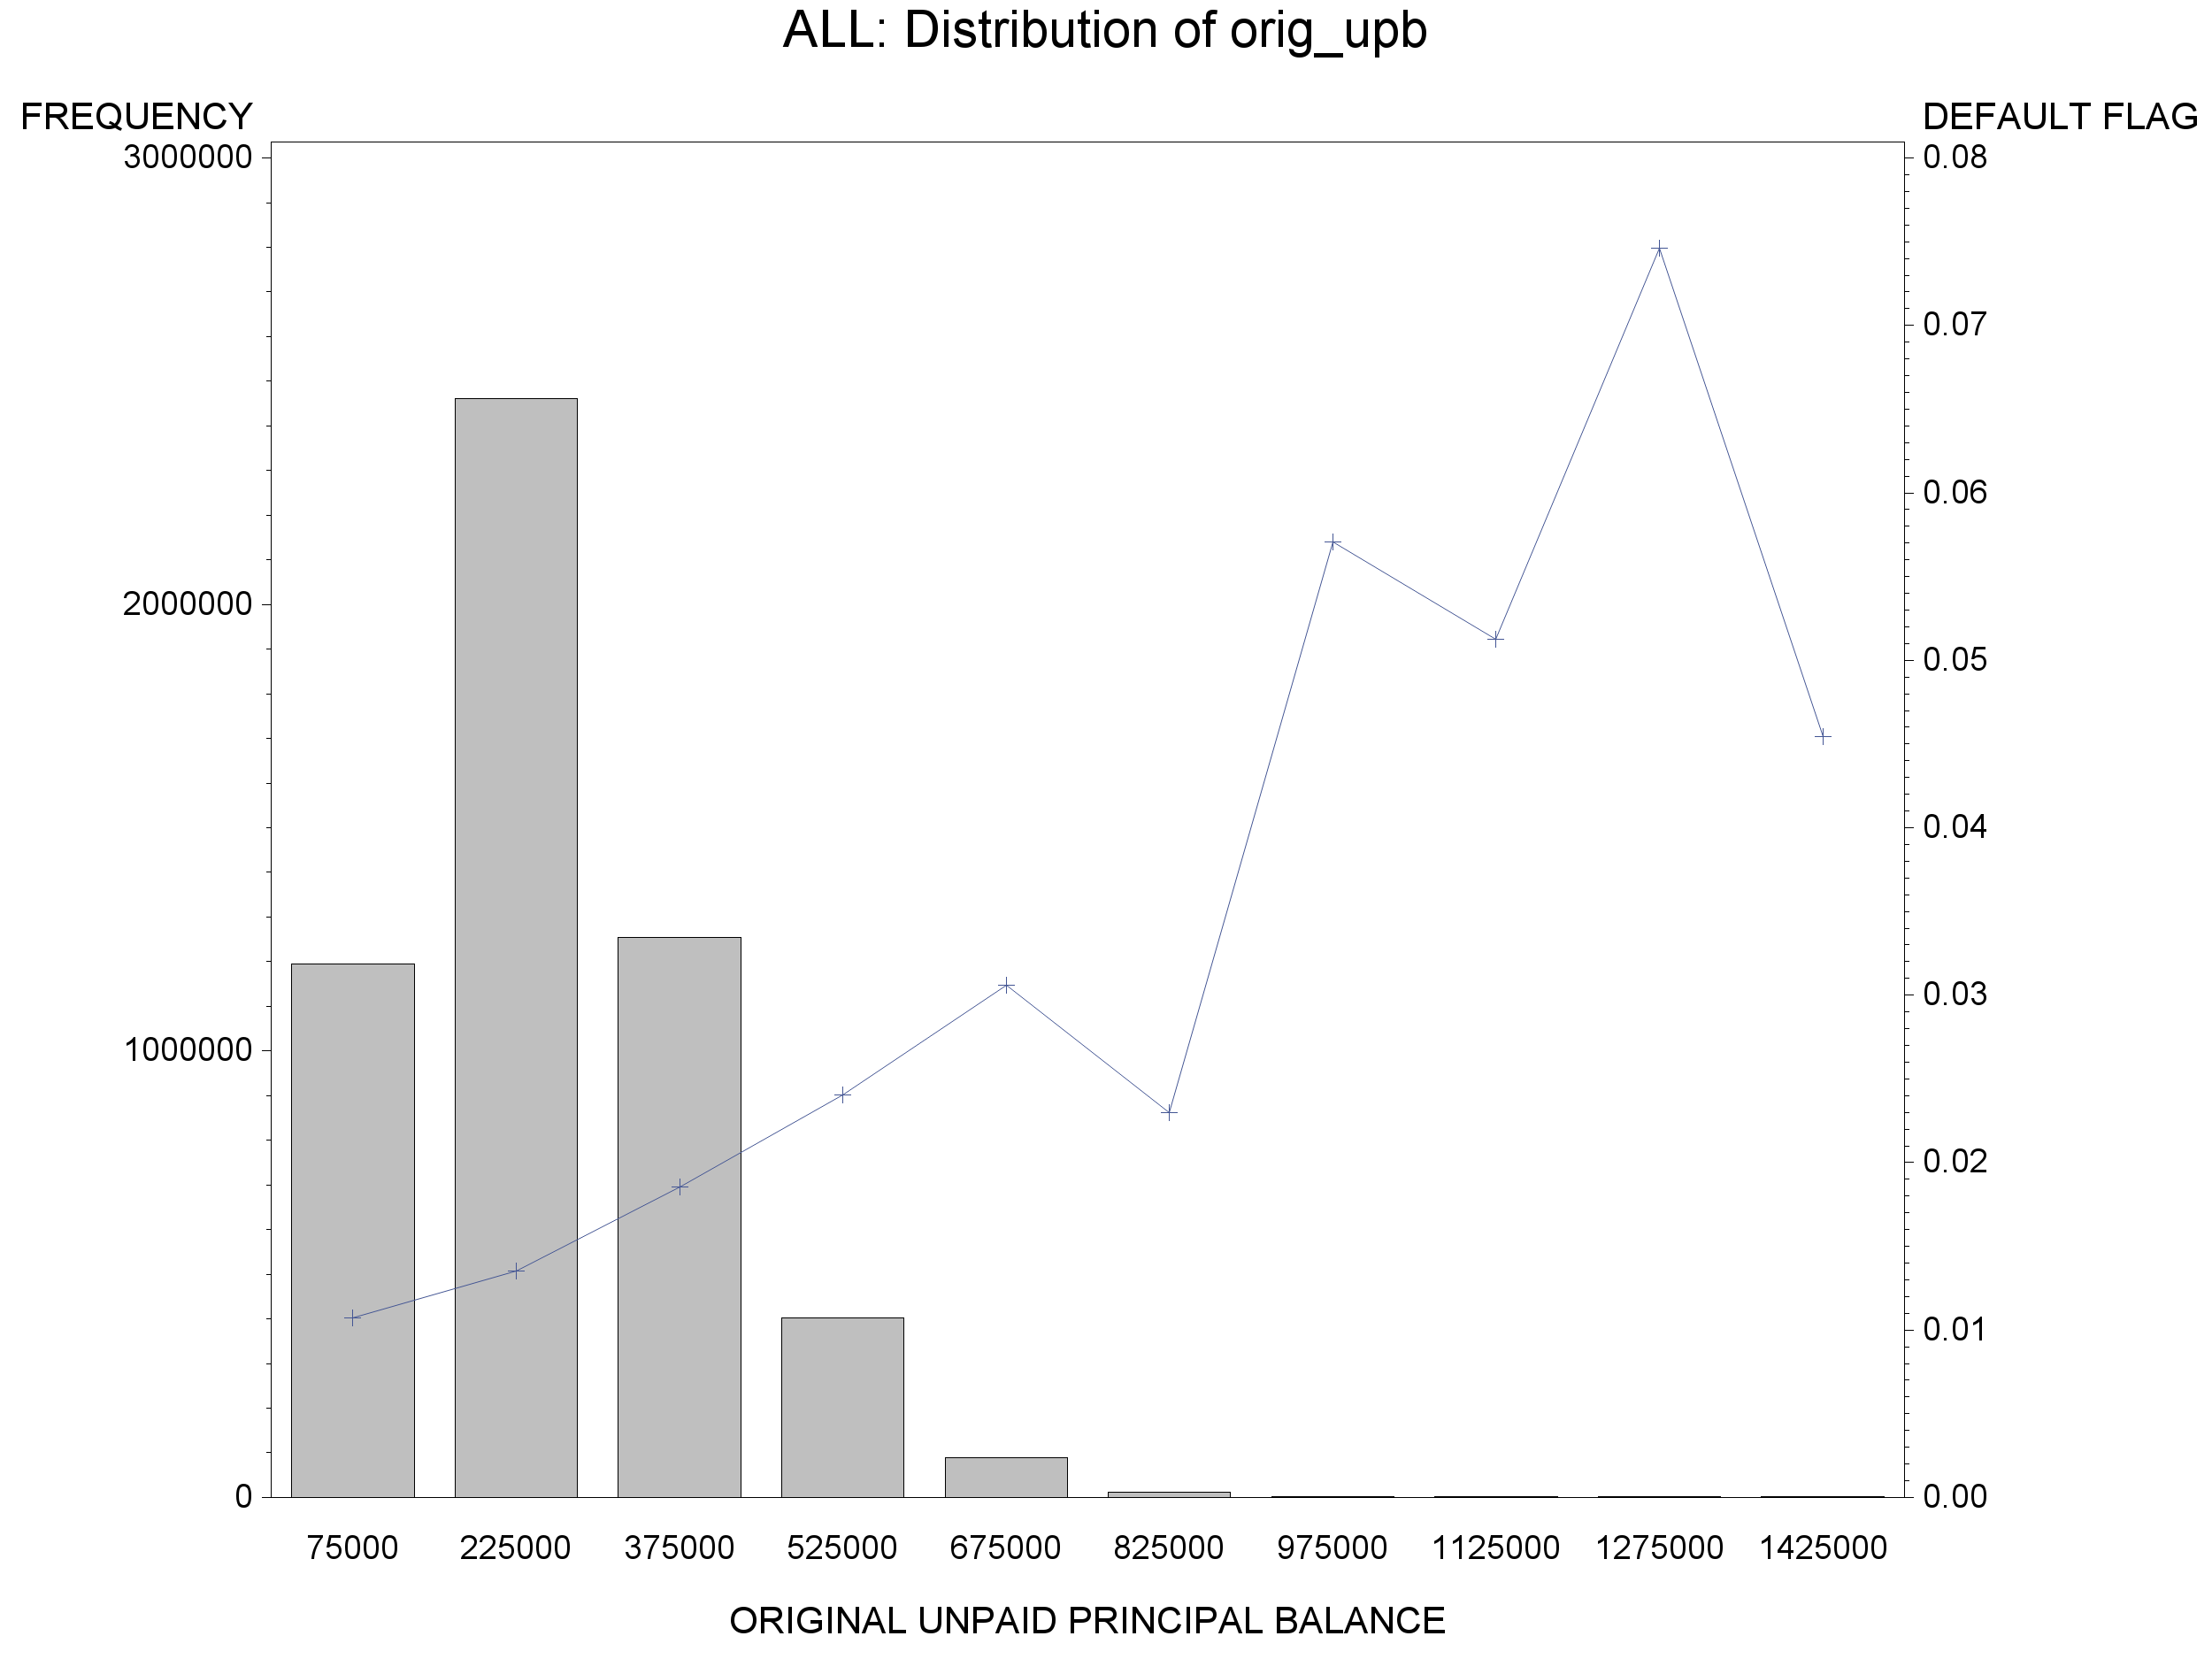
\includegraphics[width=0.9\textwidth]{./plot/Distribution/Main/RE_NUM_orig_upb_DISTRIBUTION_ALL.png}
\end{minipage}
    \caption{Distribution of Credit Score (fico) and Original UPB}
    \label{fig:re_distr1}
\end{figure}
\begin{figure}[H]
\begin{minipage}{.5\textwidth}
	\centering
	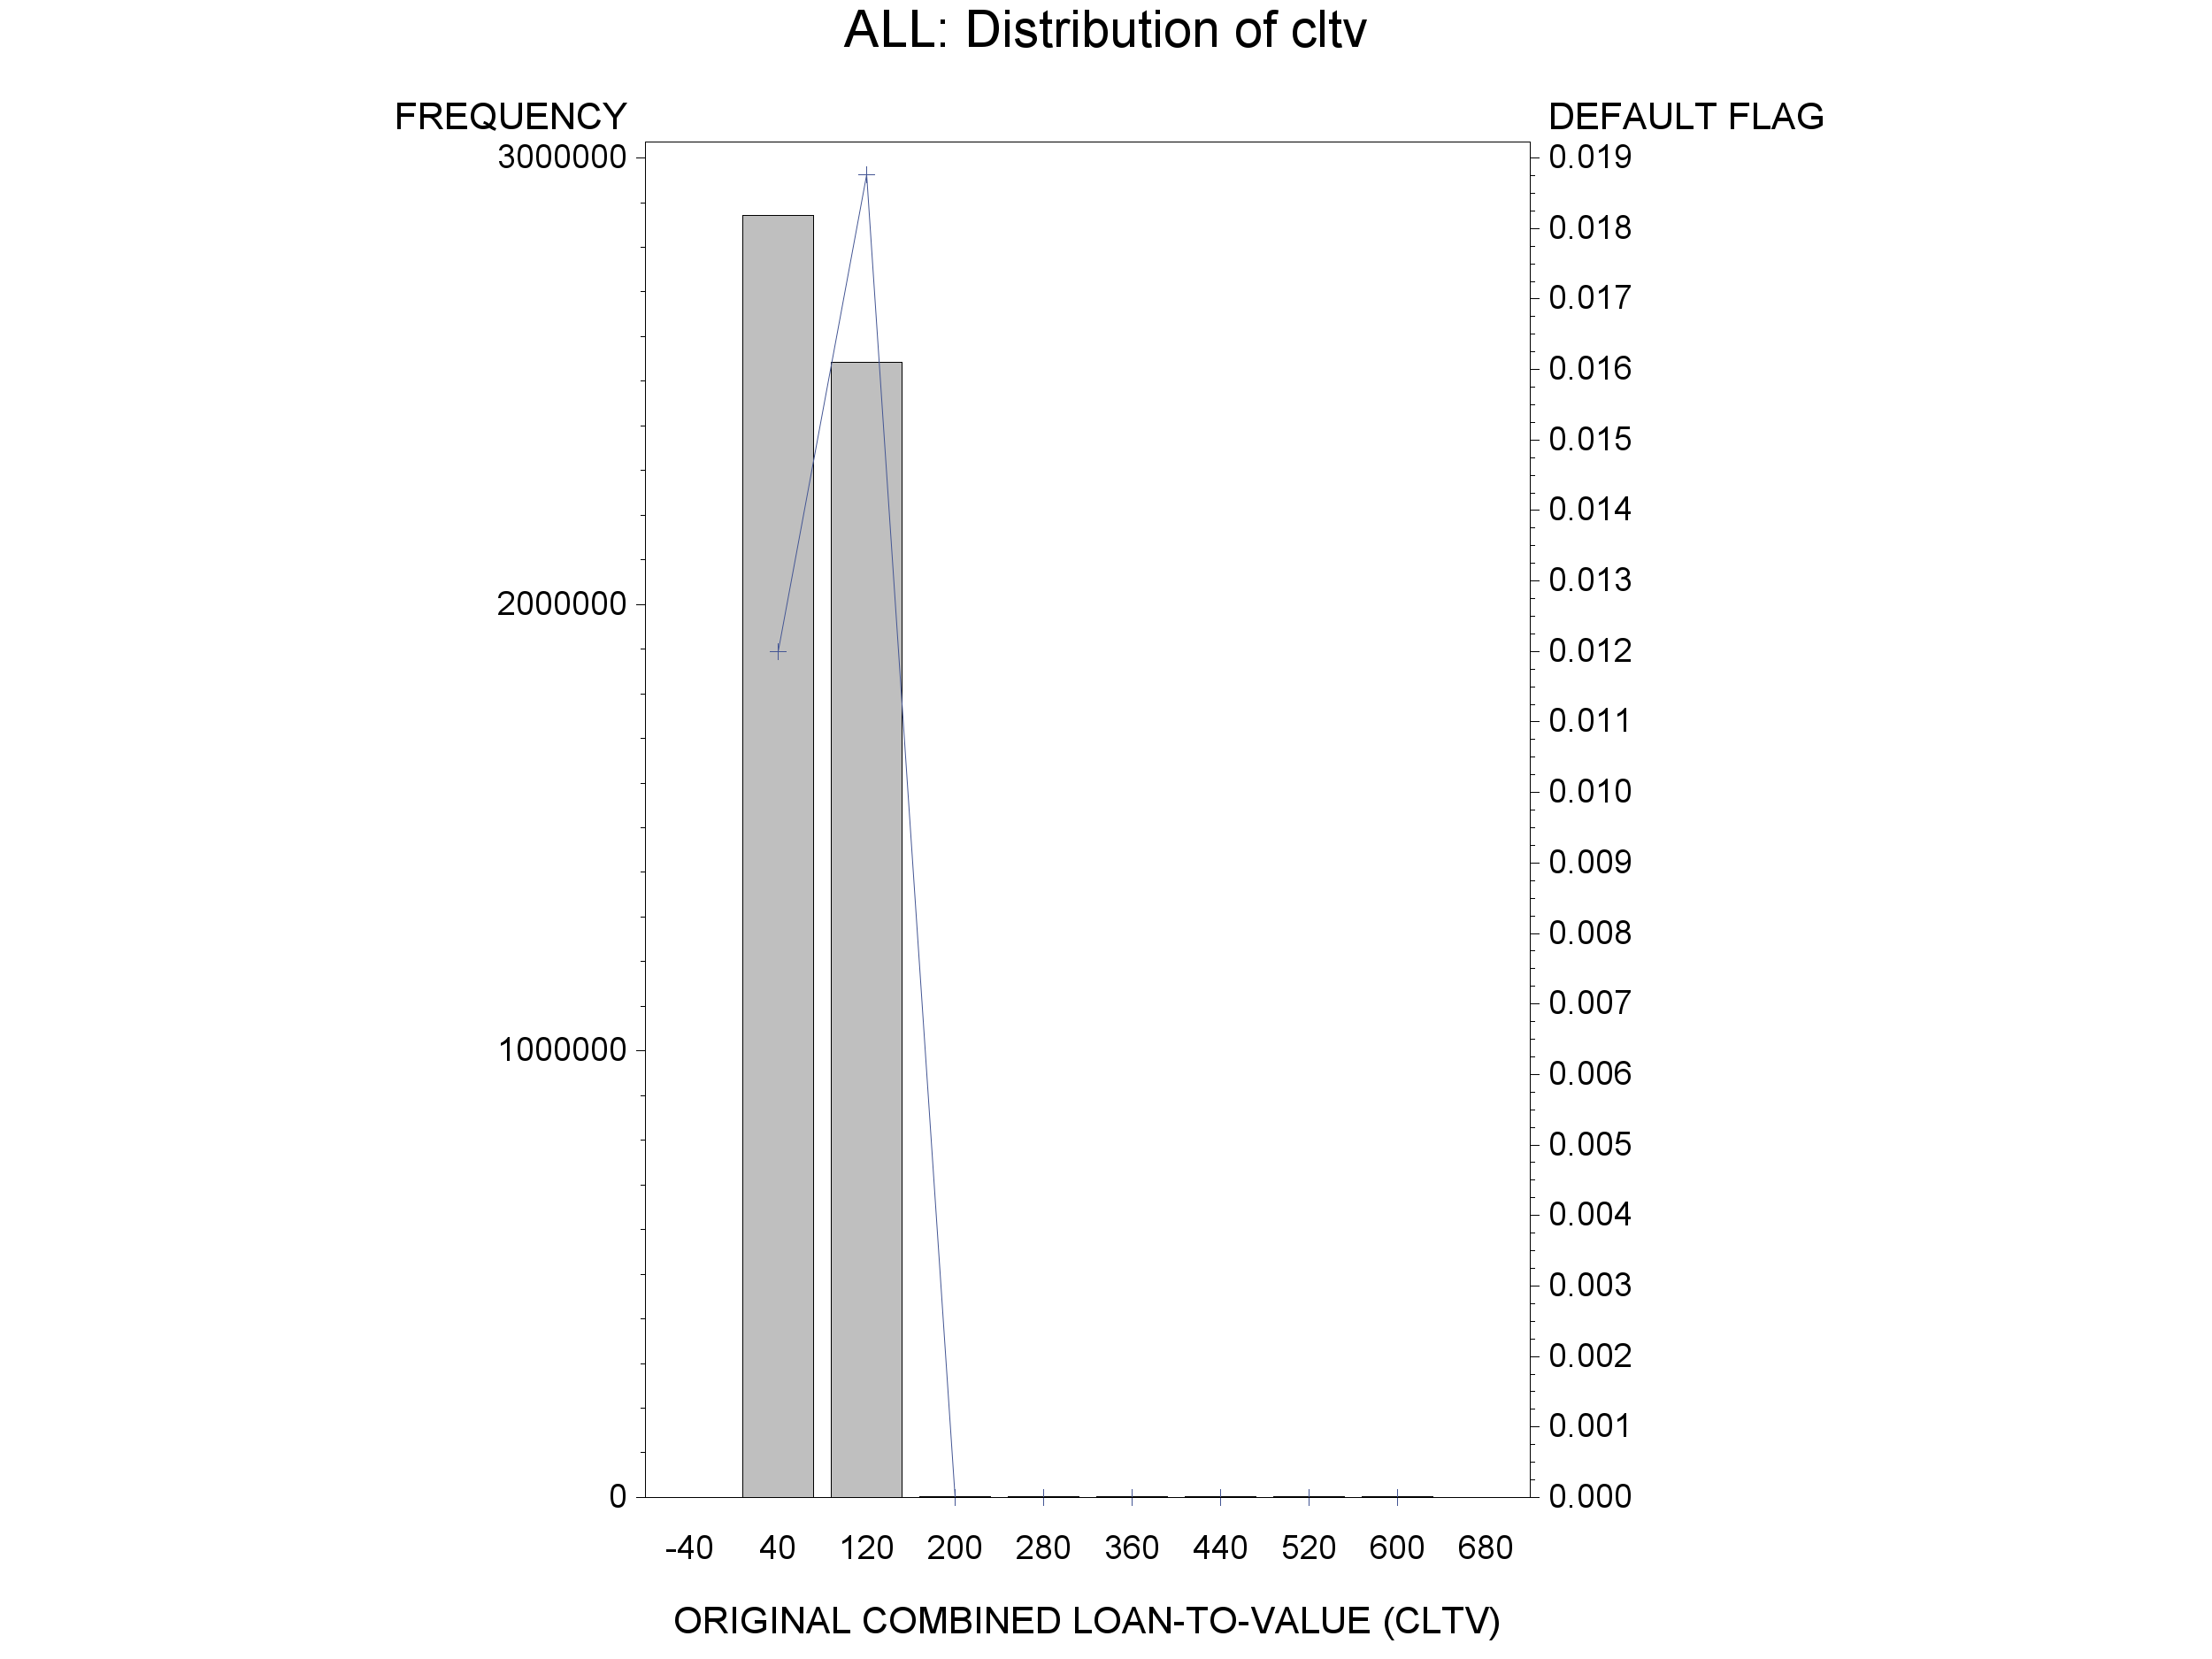
\includegraphics[width=0.9\textwidth]{./plot/Distribution/Main/RE_NUM_cltv_DISTRIBUTION_ALL.png}
\end{minipage}%
\begin{minipage}{.5\textwidth}
	\centering
	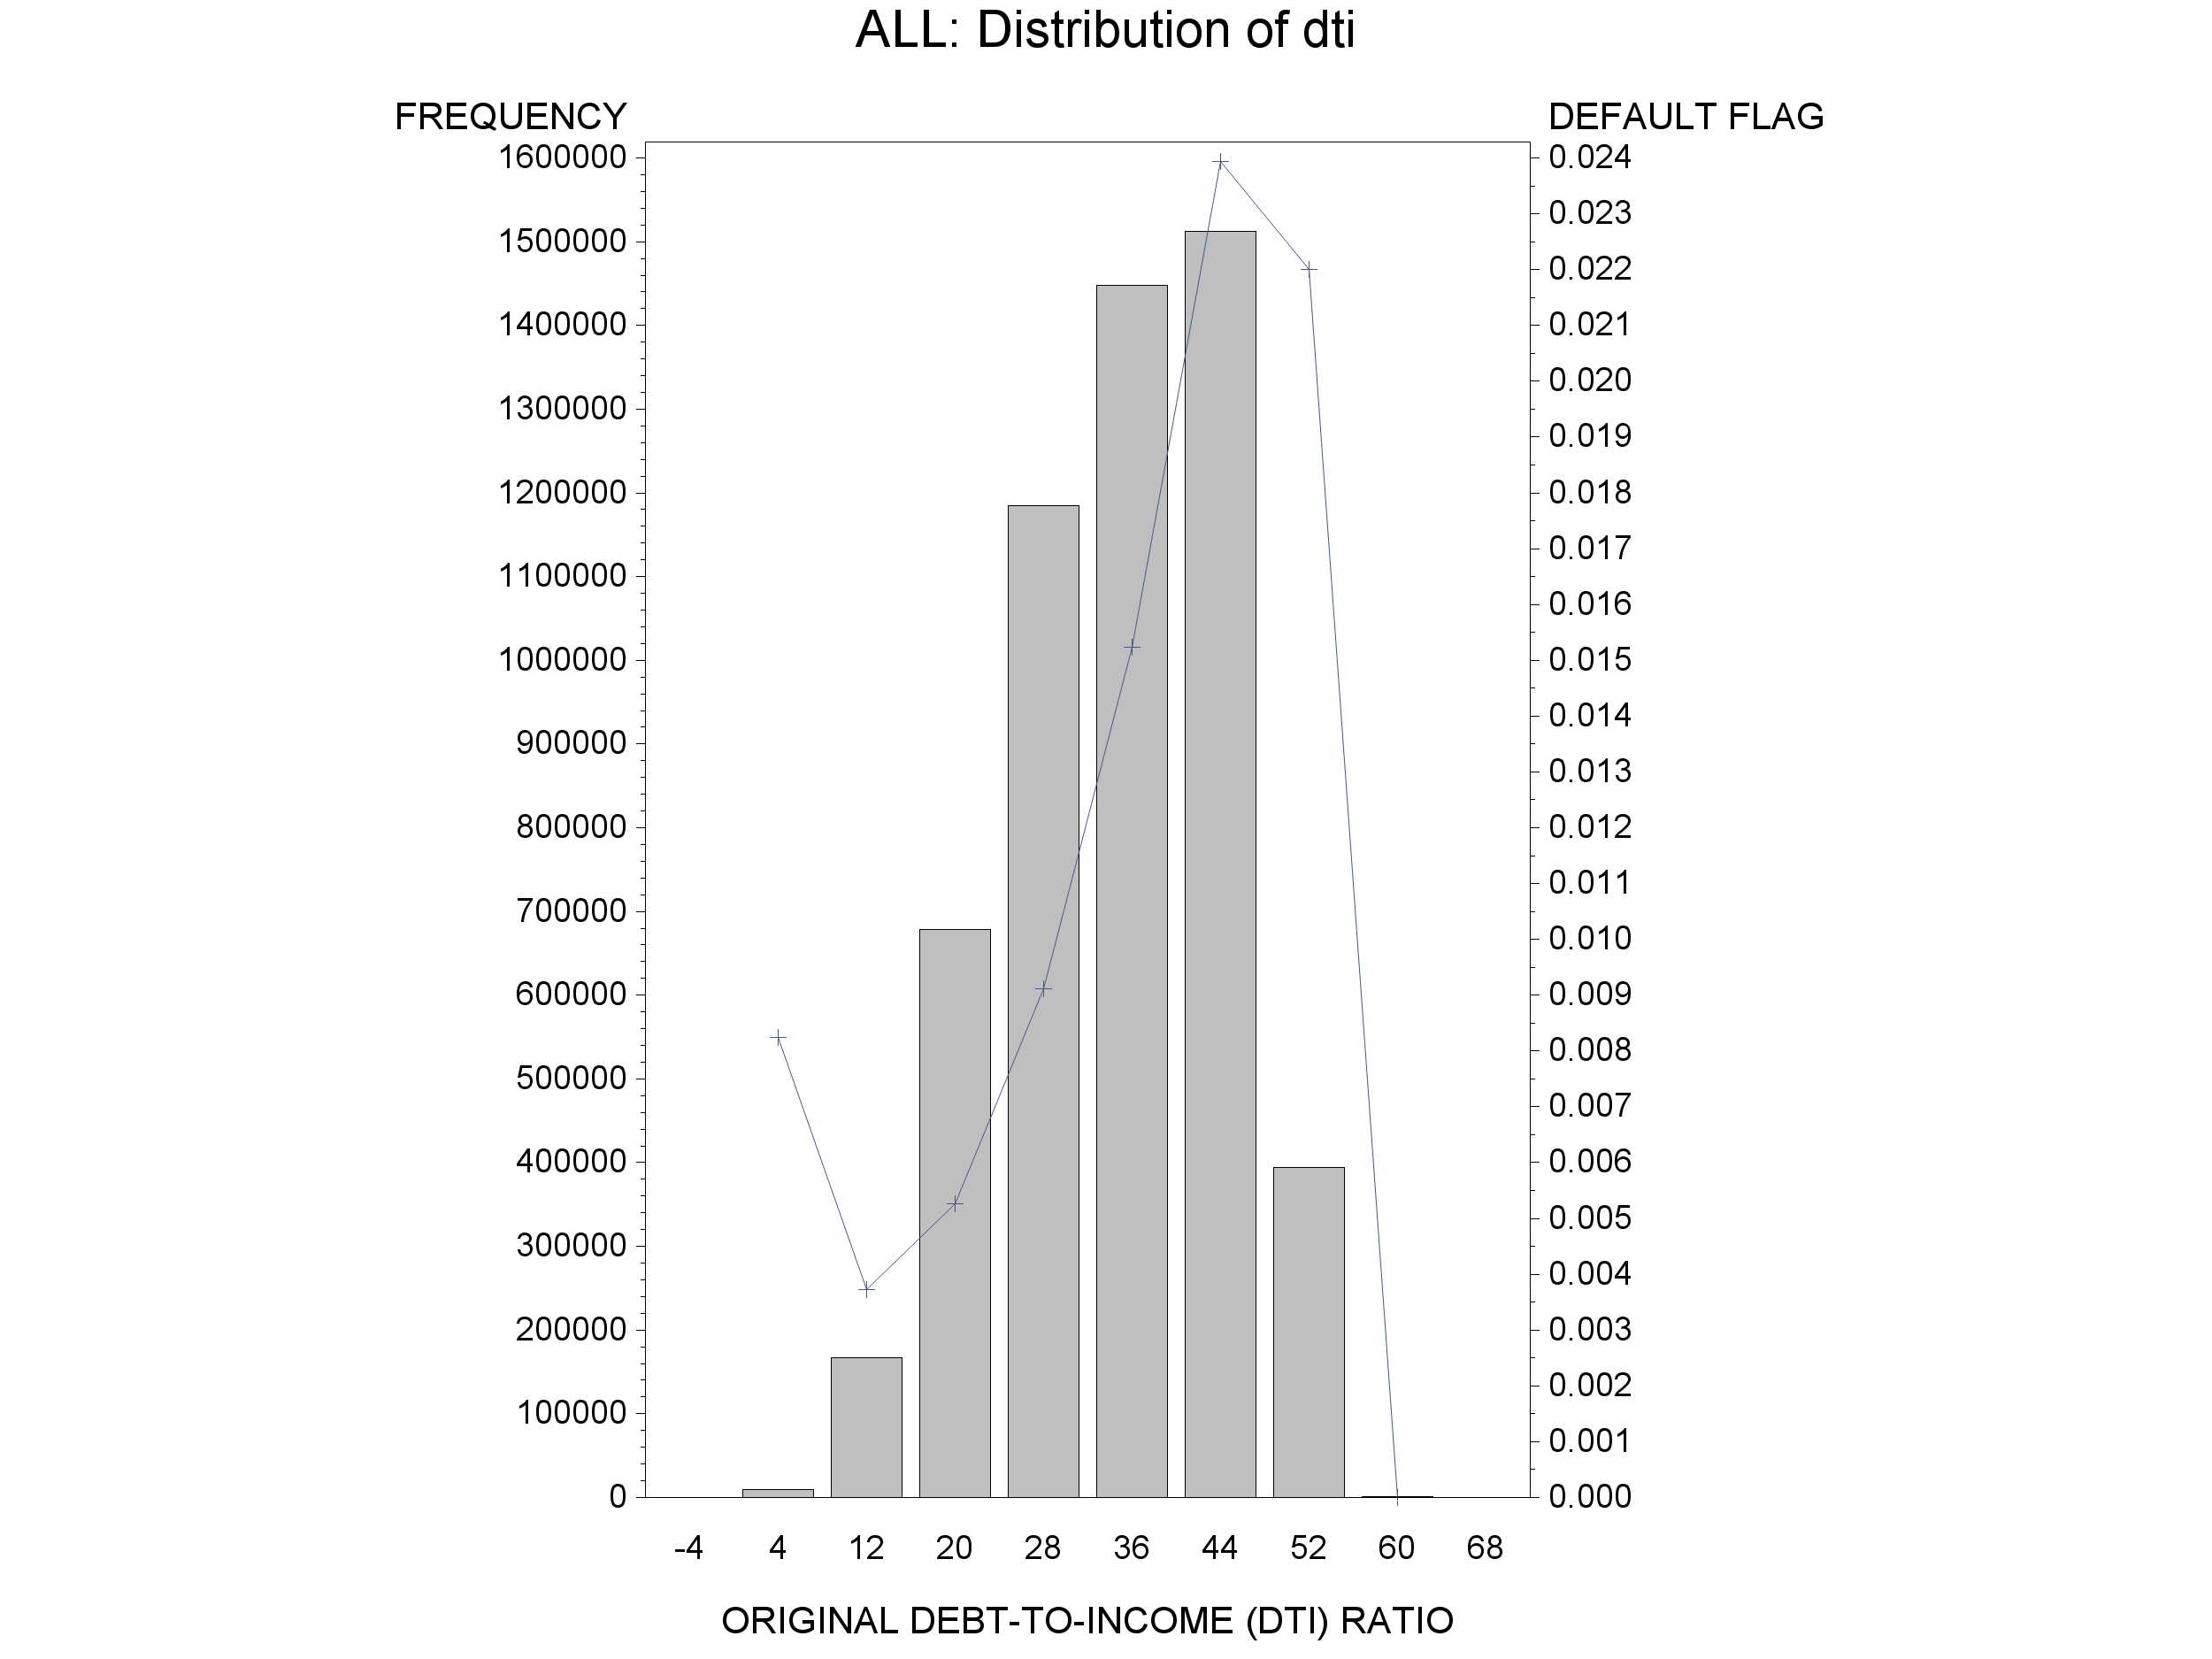
\includegraphics[width=0.9\textwidth]{./plot/Distribution/Main/RE_NUM_dti_DISTRIBUTION_ALL.png}
\end{minipage}
    \caption{Distribution of CLTV and DTI}
    %\label{fig:dp_iqr_boxpl}
\end{figure}
\begin{figure}[H]
\begin{minipage}{.5\textwidth}
	\centering
	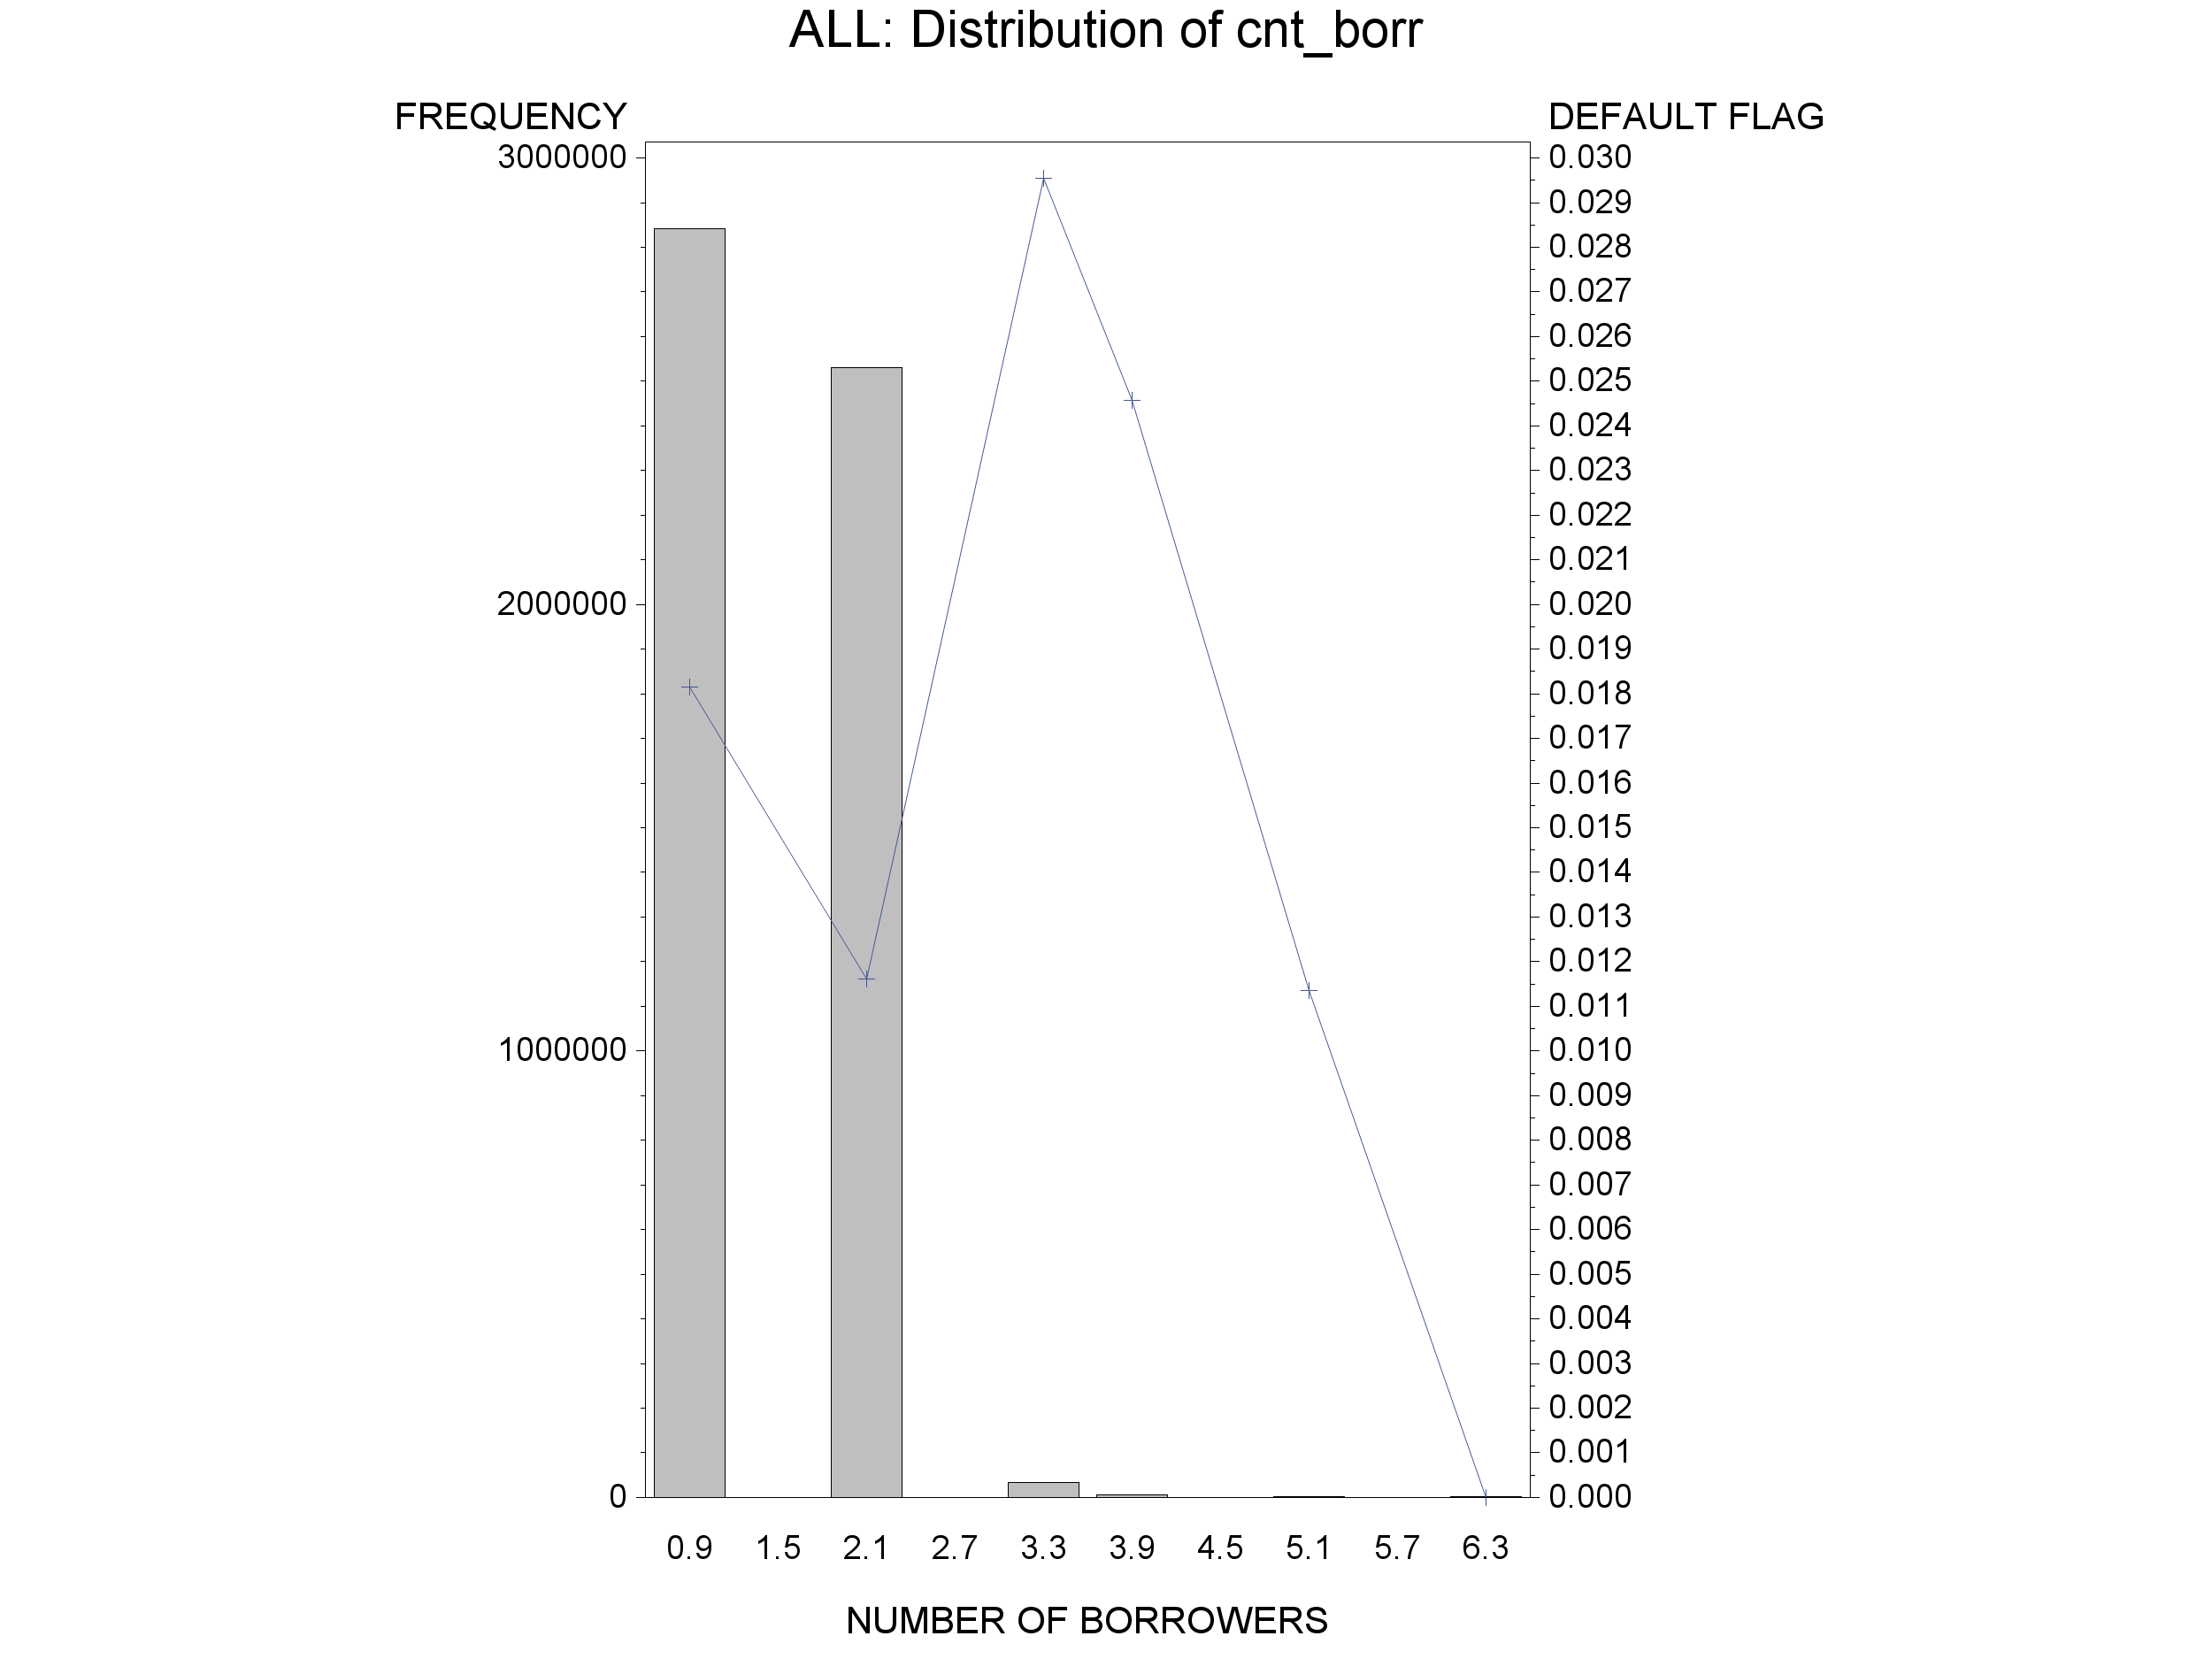
\includegraphics[width=0.9\textwidth]{./plot/Distribution/Main/RE_NUM_cnt_borr_DISTRIBUTION_ALL.png}
\end{minipage}%
\begin{minipage}{.5\textwidth}
	\centering
	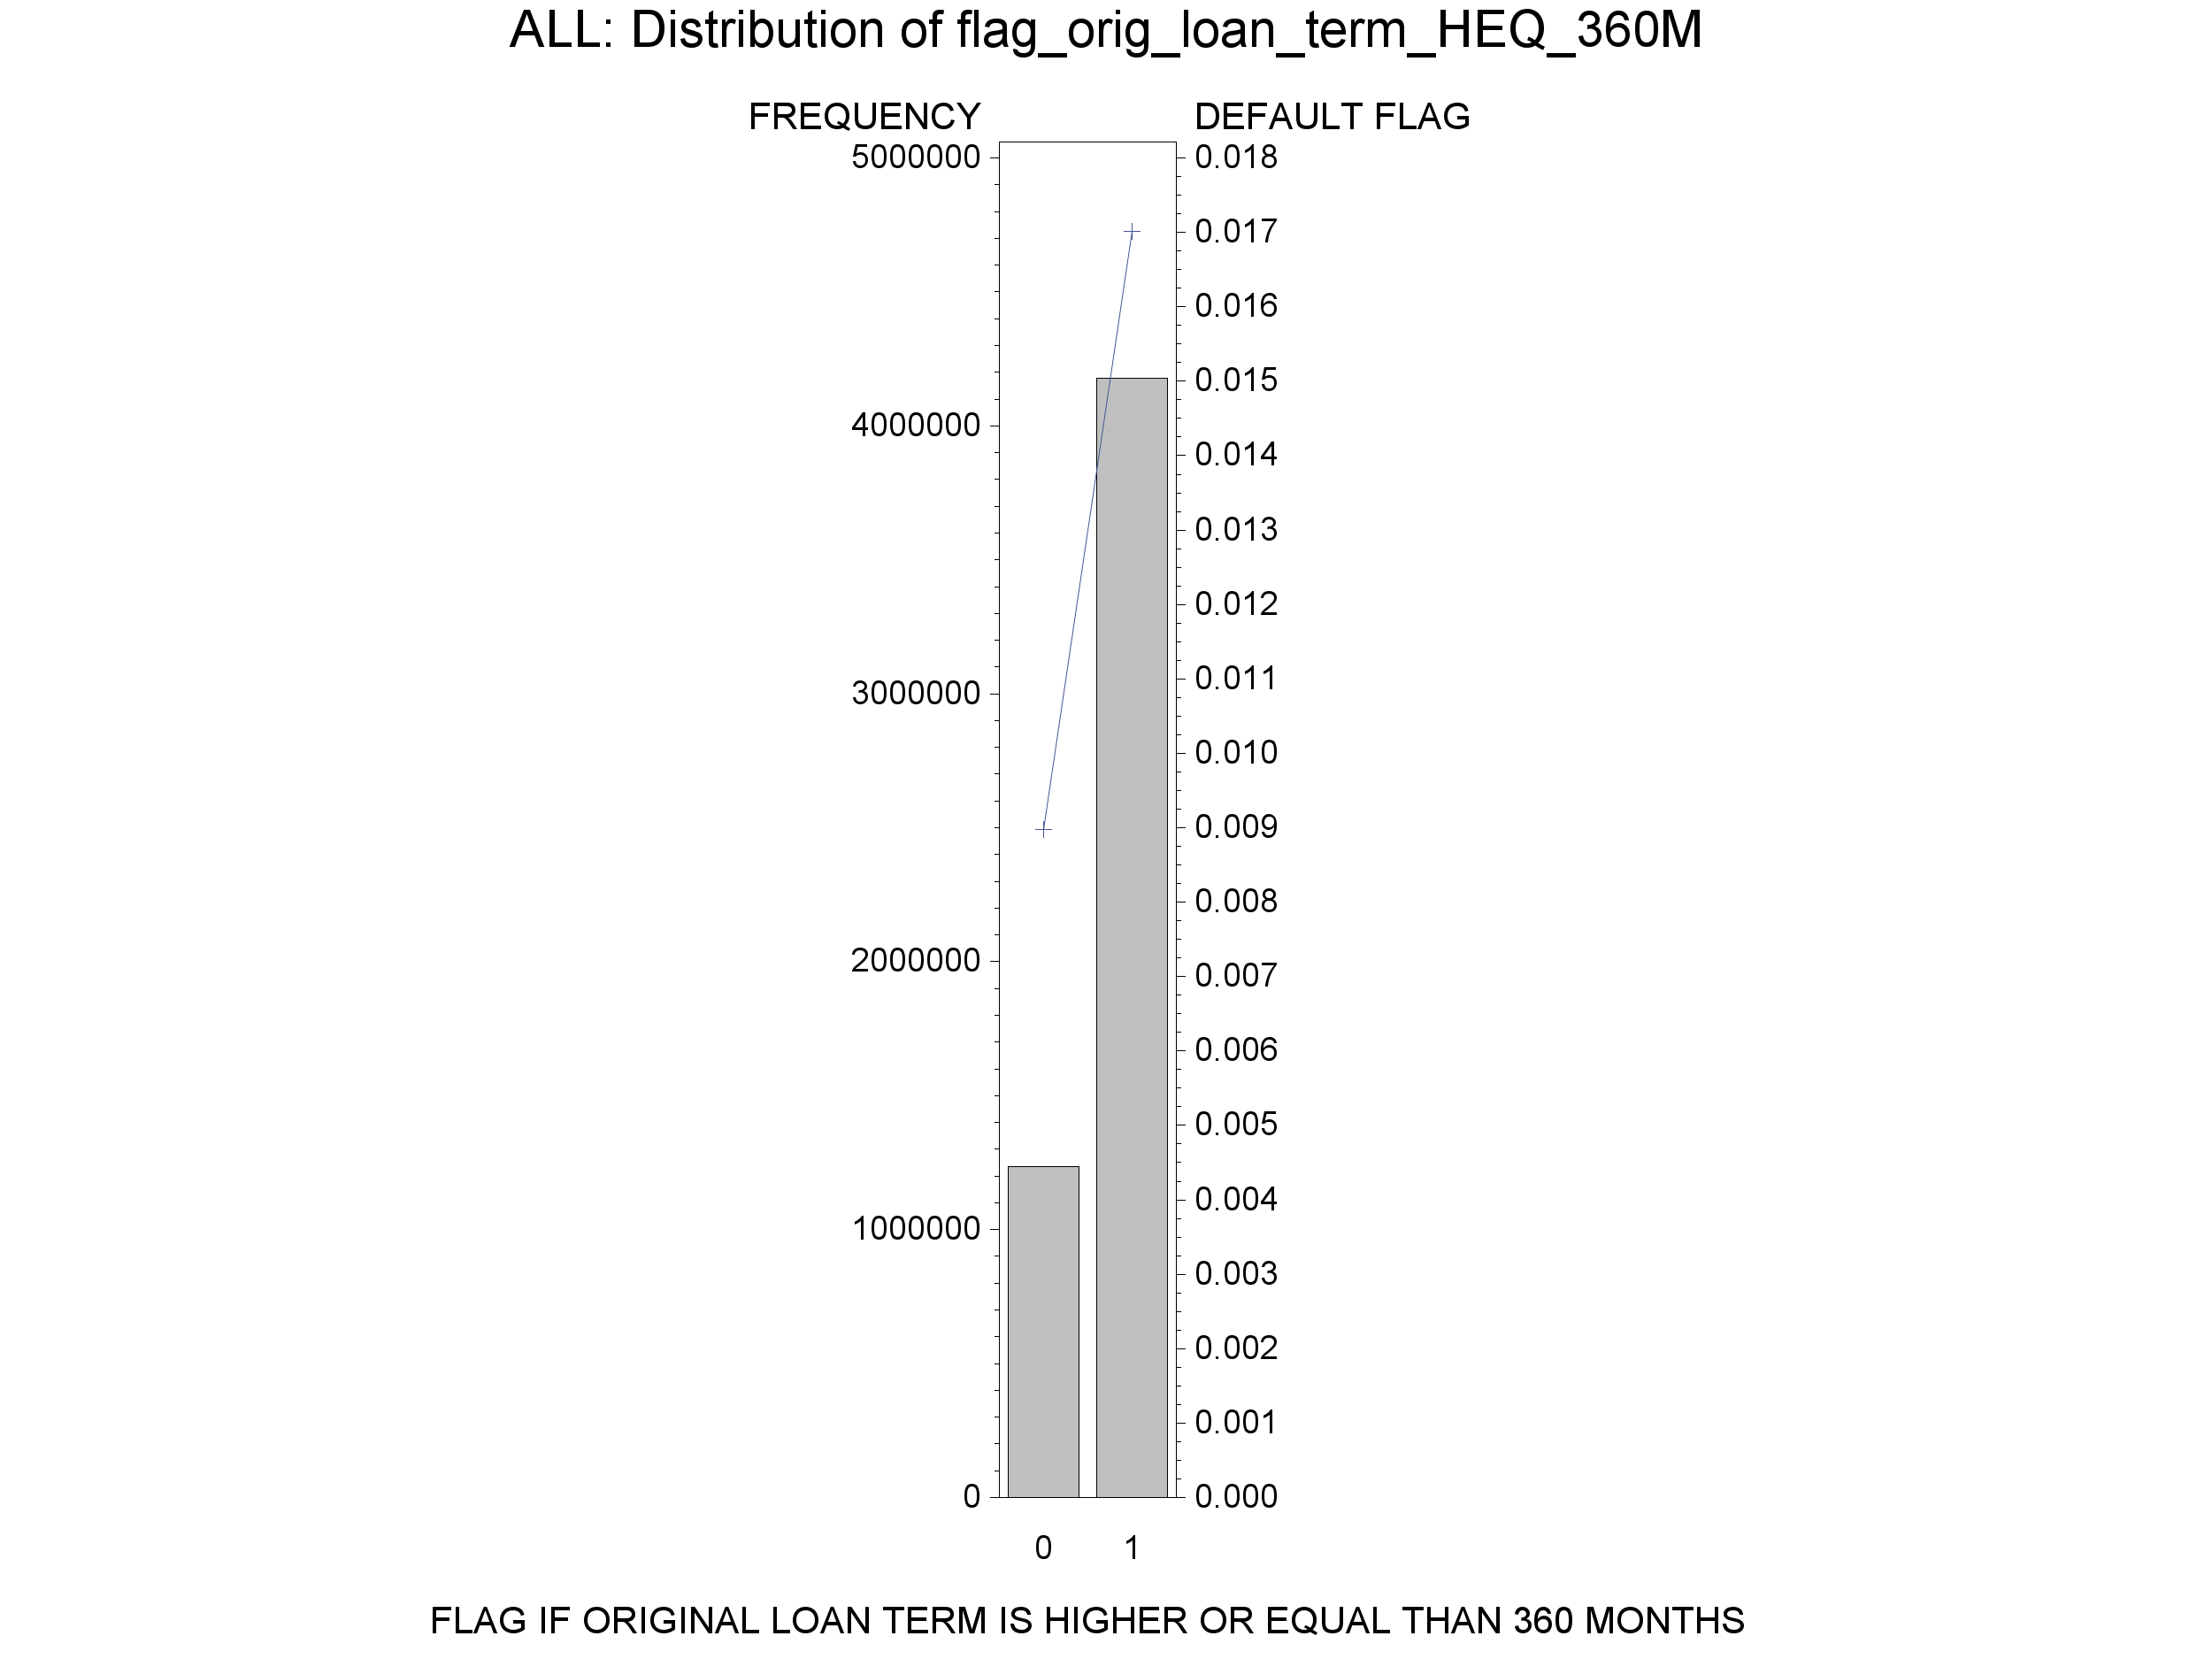
\includegraphics[width=0.9\textwidth]{./plot/Distribution/Main/RE_IND_flag_orig_loan_term_HEQ_360M_DISTRIBUTION_ALL.png}
\end{minipage}
    \caption{Distribution of Number of borrowers and Flag Original Loan Term $\geq$ 360 months}
    %\label{fig:dp_iqr_boxpl}
\end{figure}
\begin{figure}[H]
\begin{minipage}{.5\textwidth}
	\centering
	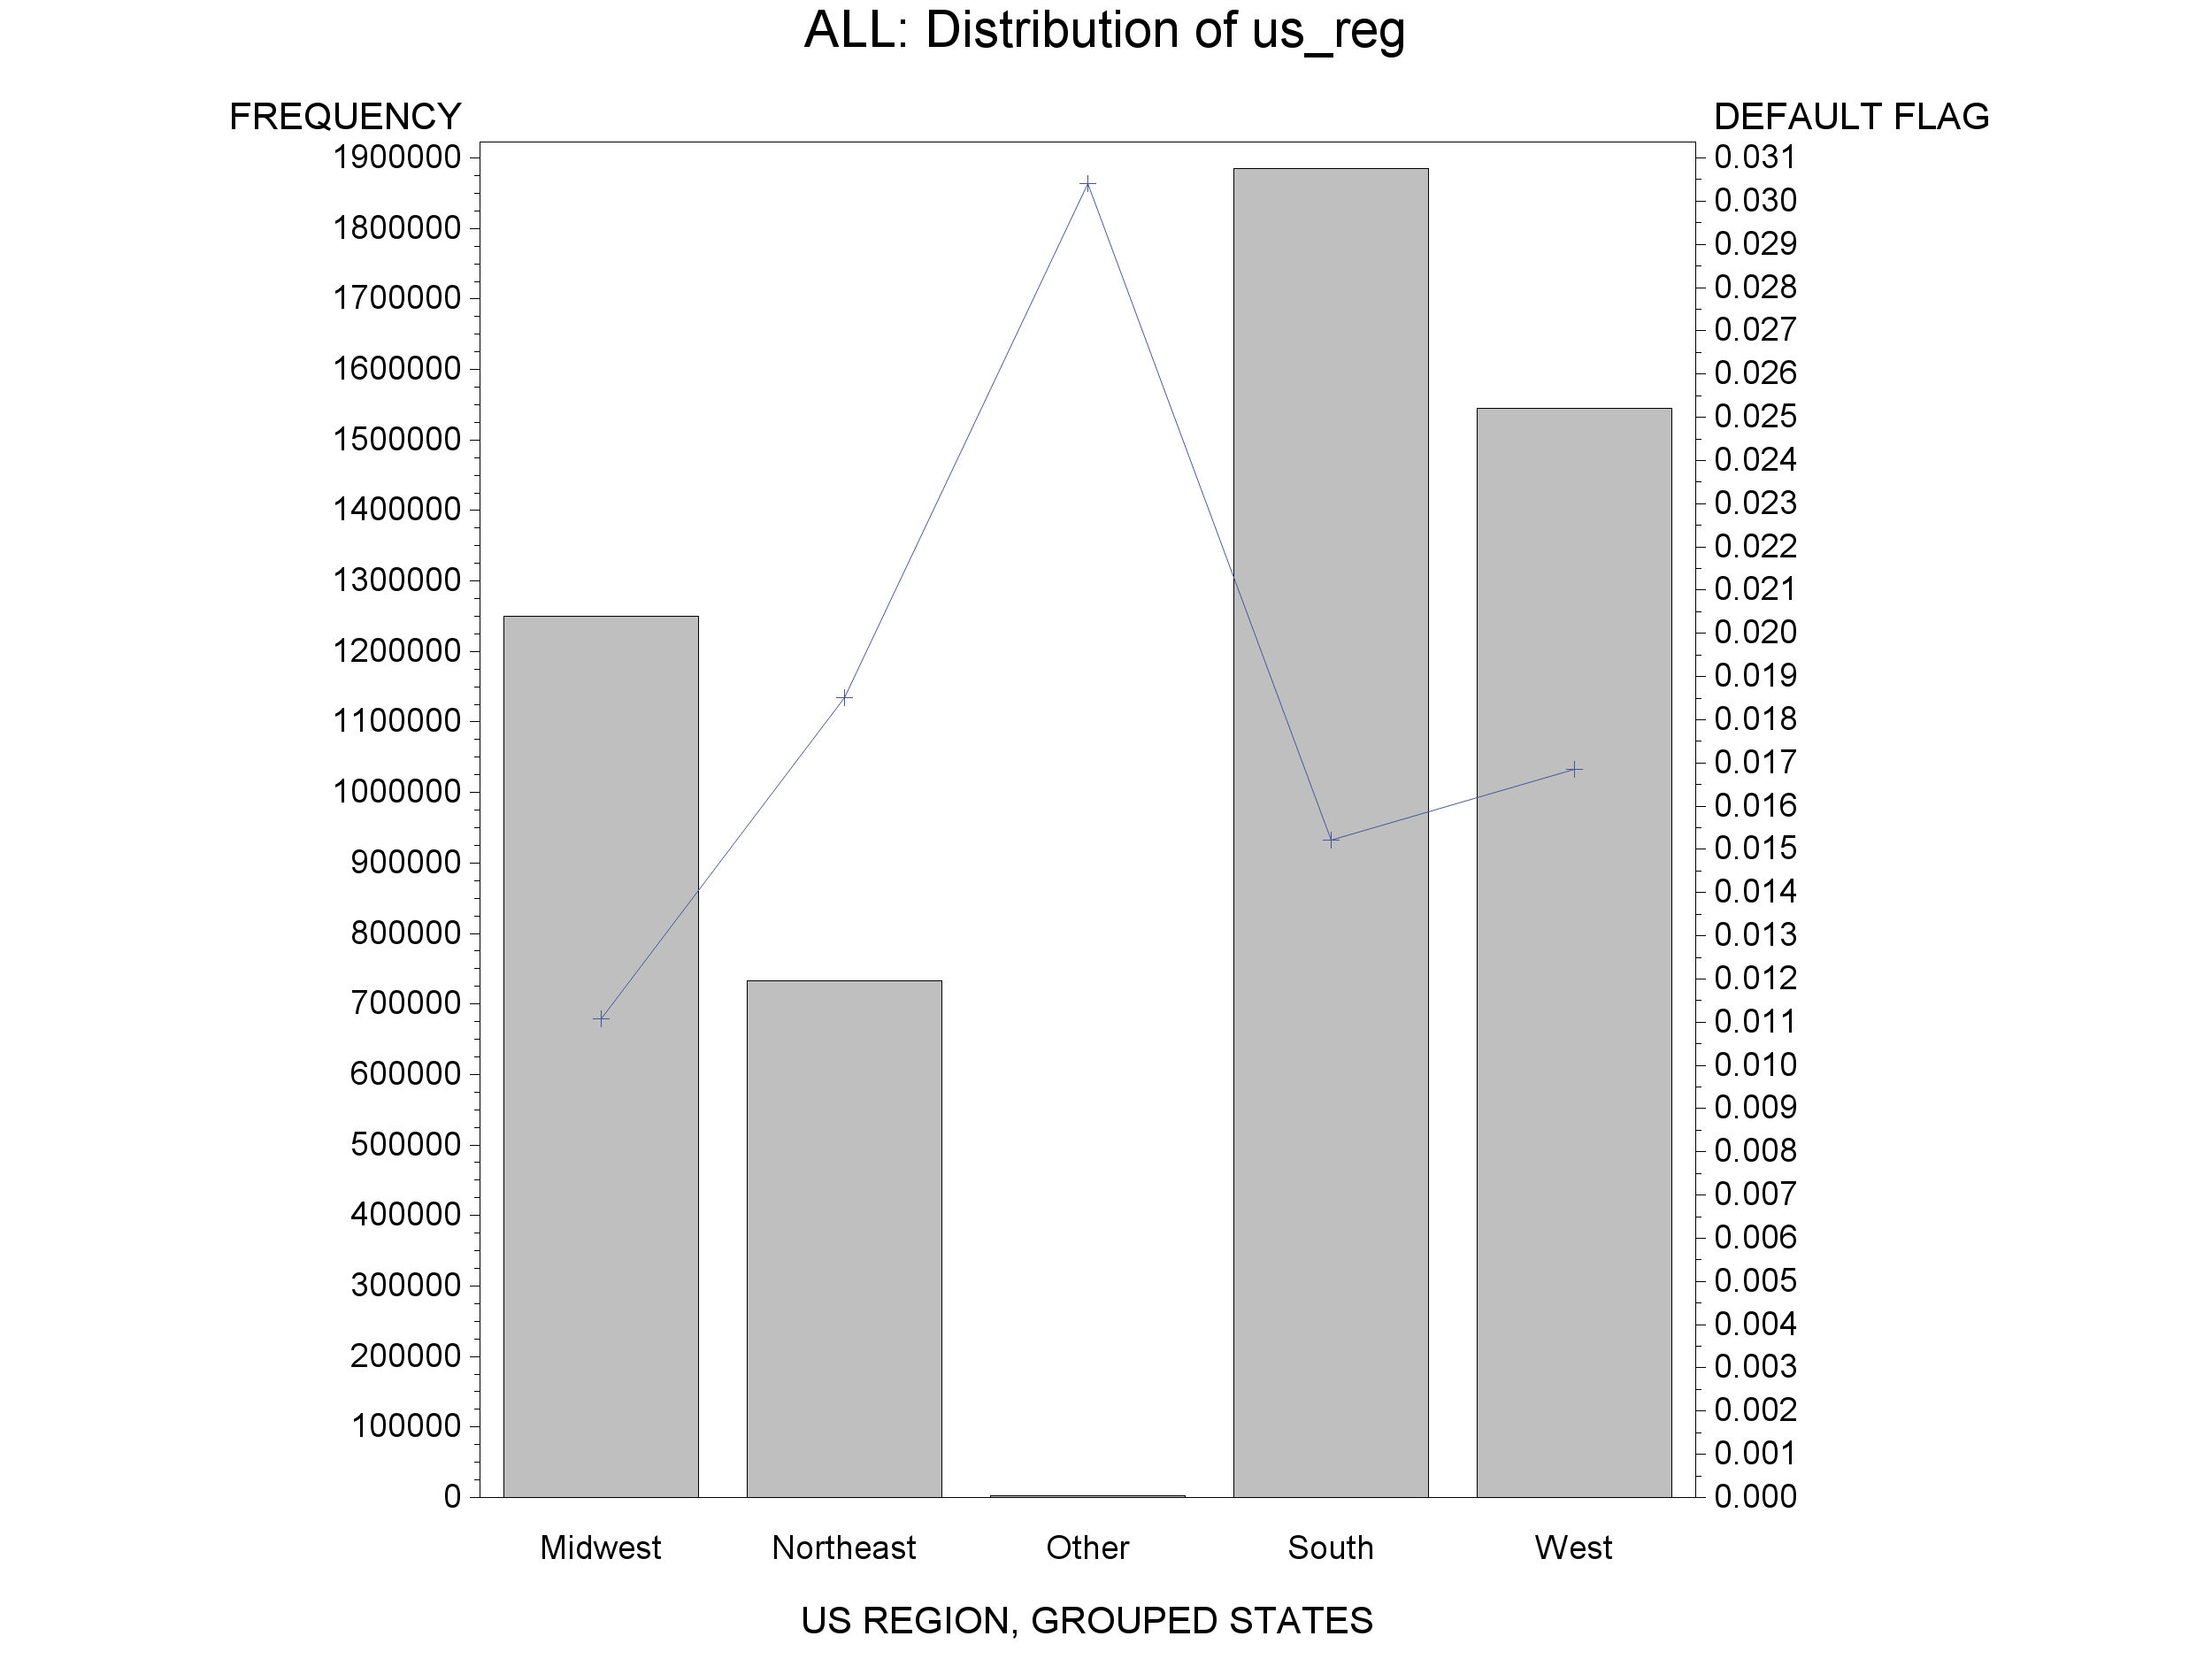
\includegraphics[width=0.9\textwidth]{./plot/Distribution/Main/RE_CAT_us_reg_DISTRIBUTION_ALL.png}
\end{minipage}%
\begin{minipage}{.5\textwidth}
	\centering
	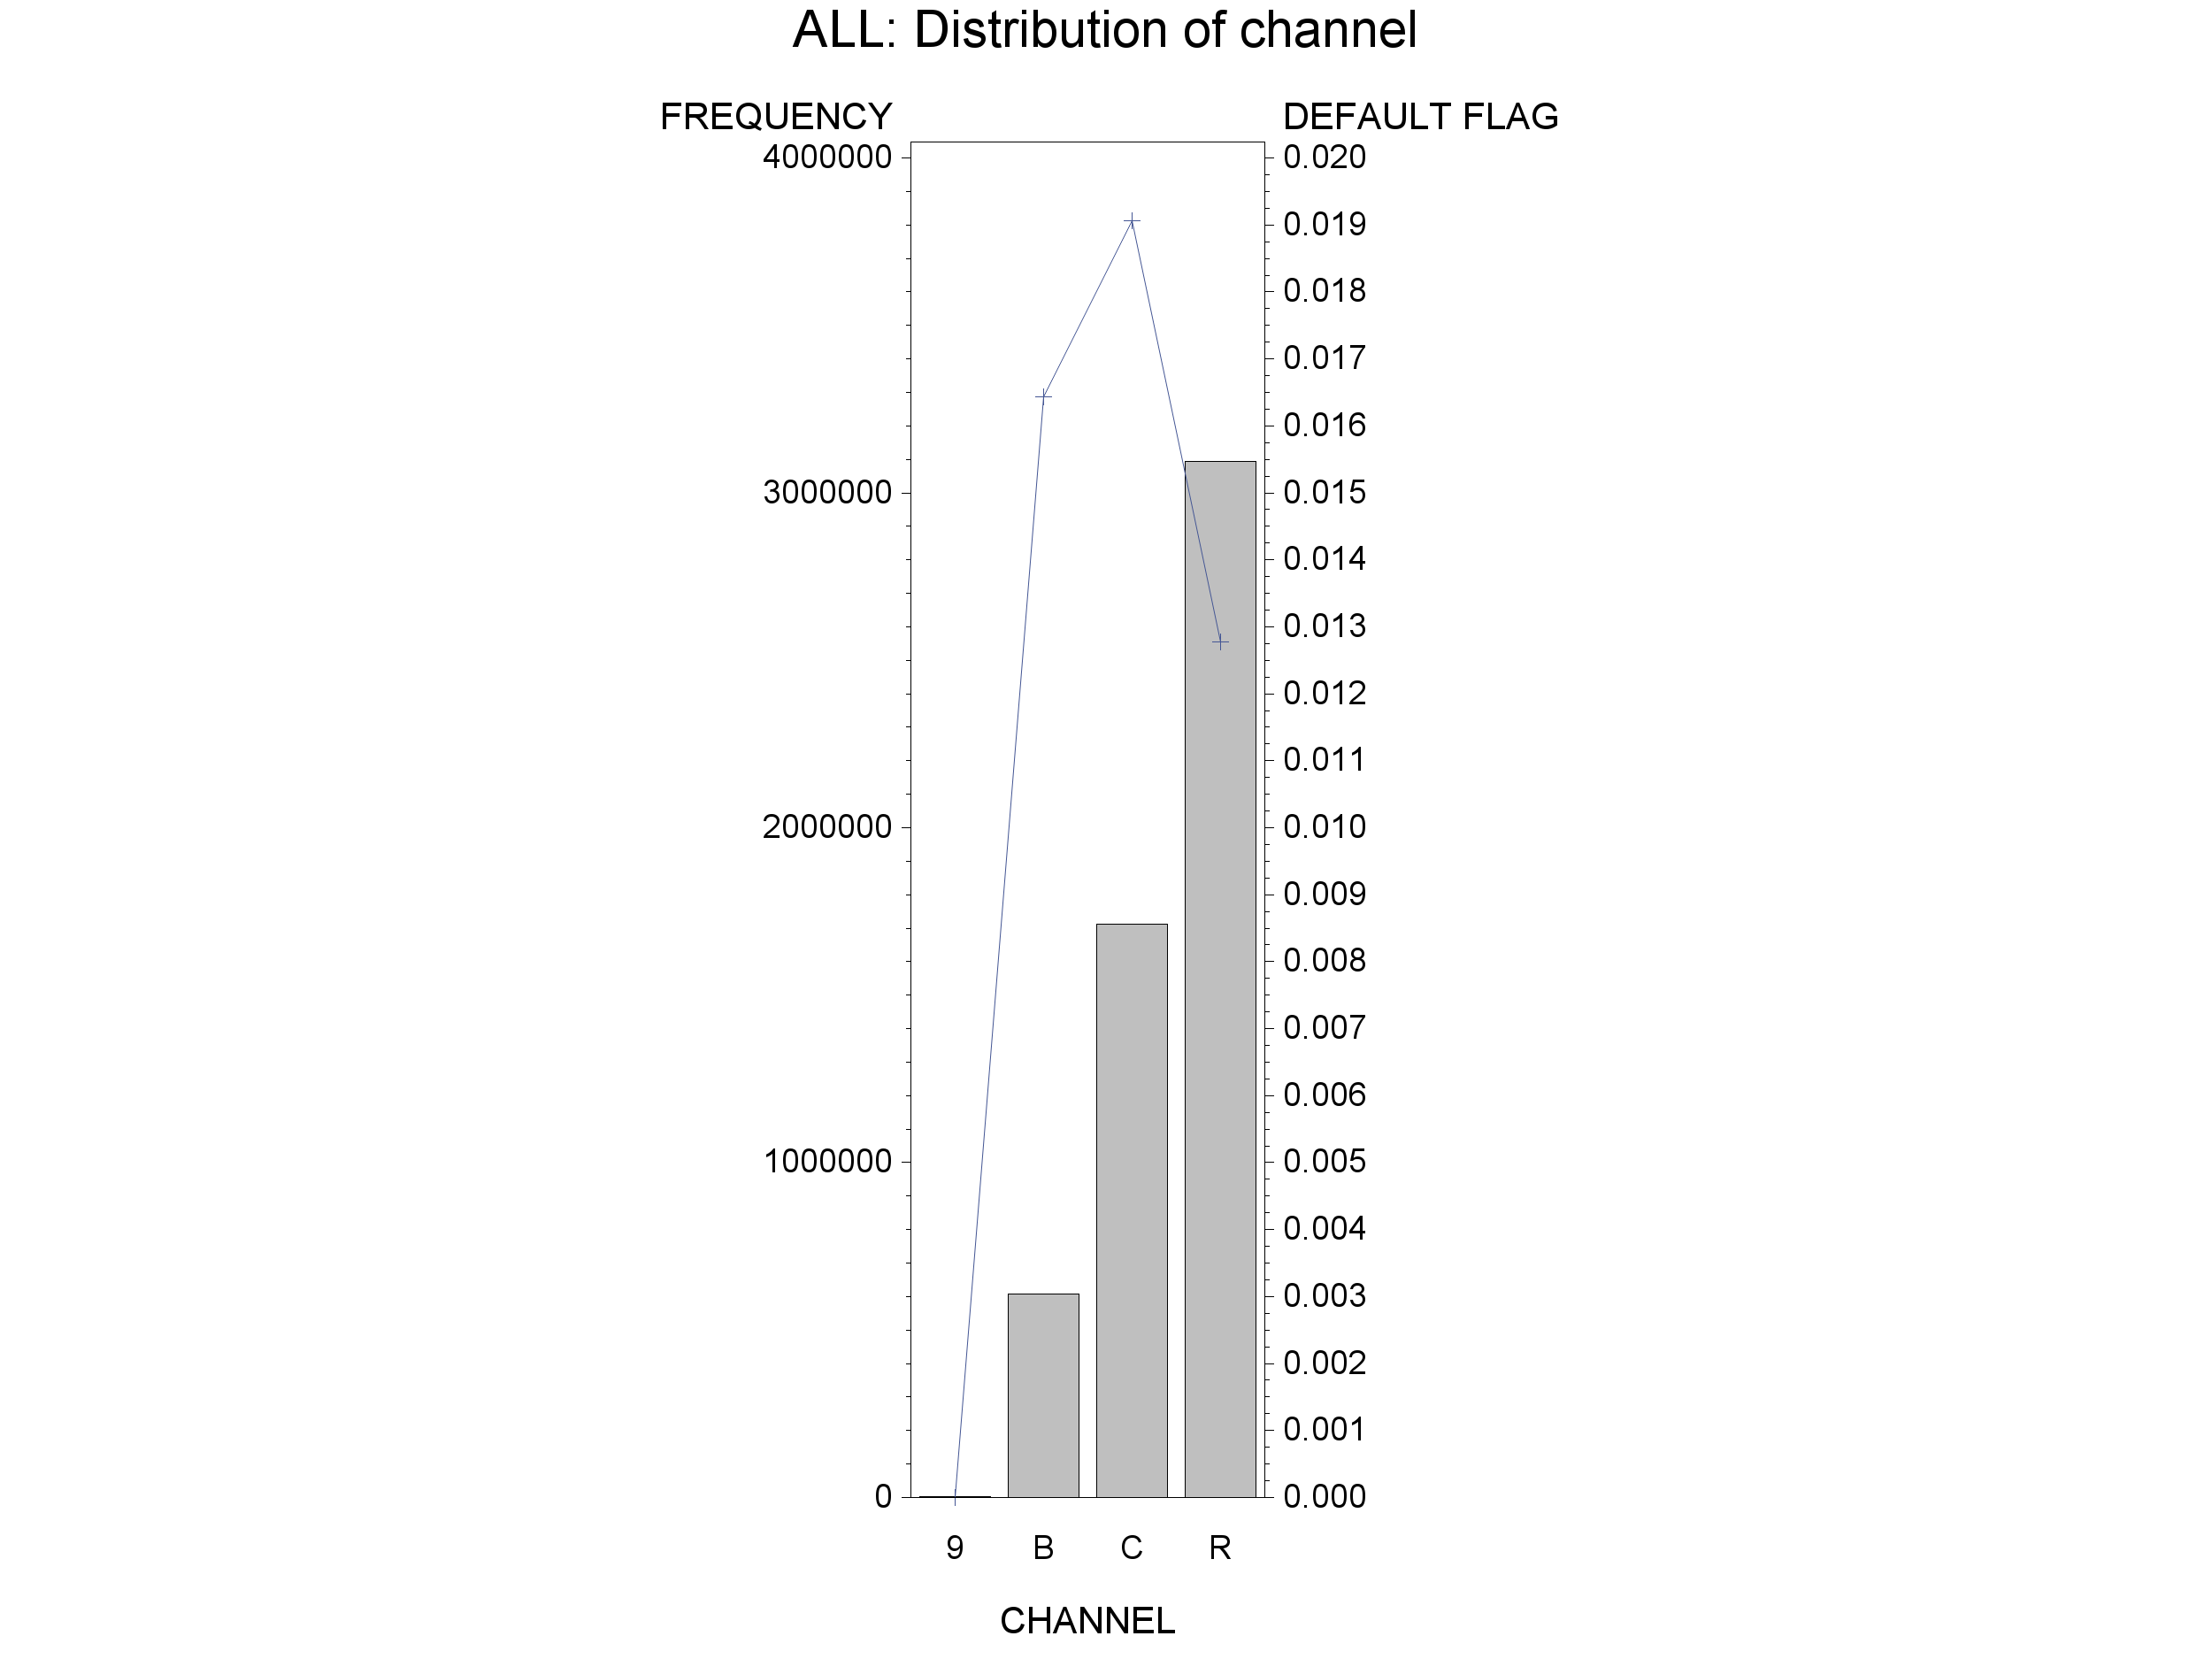
\includegraphics[width=0.9\textwidth]{./plot/Distribution/Main/RE_CAT_channel_DISTRIBUTION_ALL.png}
\end{minipage}
    \caption{Distribution of US region and Channel}
    \label{fig:re_distr4}
\end{figure}

\subsection{Outlier Treatment}
The interquartile approach, detailed in Chapter \ref{sec:OutlTr}, was employed to identify outliers and their presentation was visualized through boxplots (Figure \ref{fig:re_boxpl_fico_origupb} - \ref{fig:re_boxpl_noborr_loanterm}, all plots in Appendix \ref{sec:boxplot_all}). Upper and lower boundaries were determined using Equations \ref{eq:dp_iqr_boxpl2} and \ref{eq:dp_iqr_boxpl2}. Quartiles for all numerical risk factors are outlined in Table \ref{tab:re_descr_stat}, with resulting limits available in Table \ref{tab:re_iqr}. The proportion of upper and lower outliers were calculated to analyze, if a significant amount of data entries are affected and could potentially impact the modeling process. While outliers were present in all numerical variables, only the risk factor \emph{Original Loan Term} shows a concerning proportion. New risk factors were derived to circumvent this issue. Multiple versions of indicator variables were created using the definition listed in Table \ref{tab:re_descr_newvar}. Additionally, after analyzing the distribution and box plots of all risk factors, a winsorization was executed to evaluate, if outliers affected the discriminatory power negatively. Therefore, data points with values above the upper or below the lower limit, were capped at their respective thresholds. The performance of the adjusted variables did not change significantly and thus, the original versions were retained.

\begin{figure}[H]
\begin{minipage}{.5\textwidth}
	\centering
	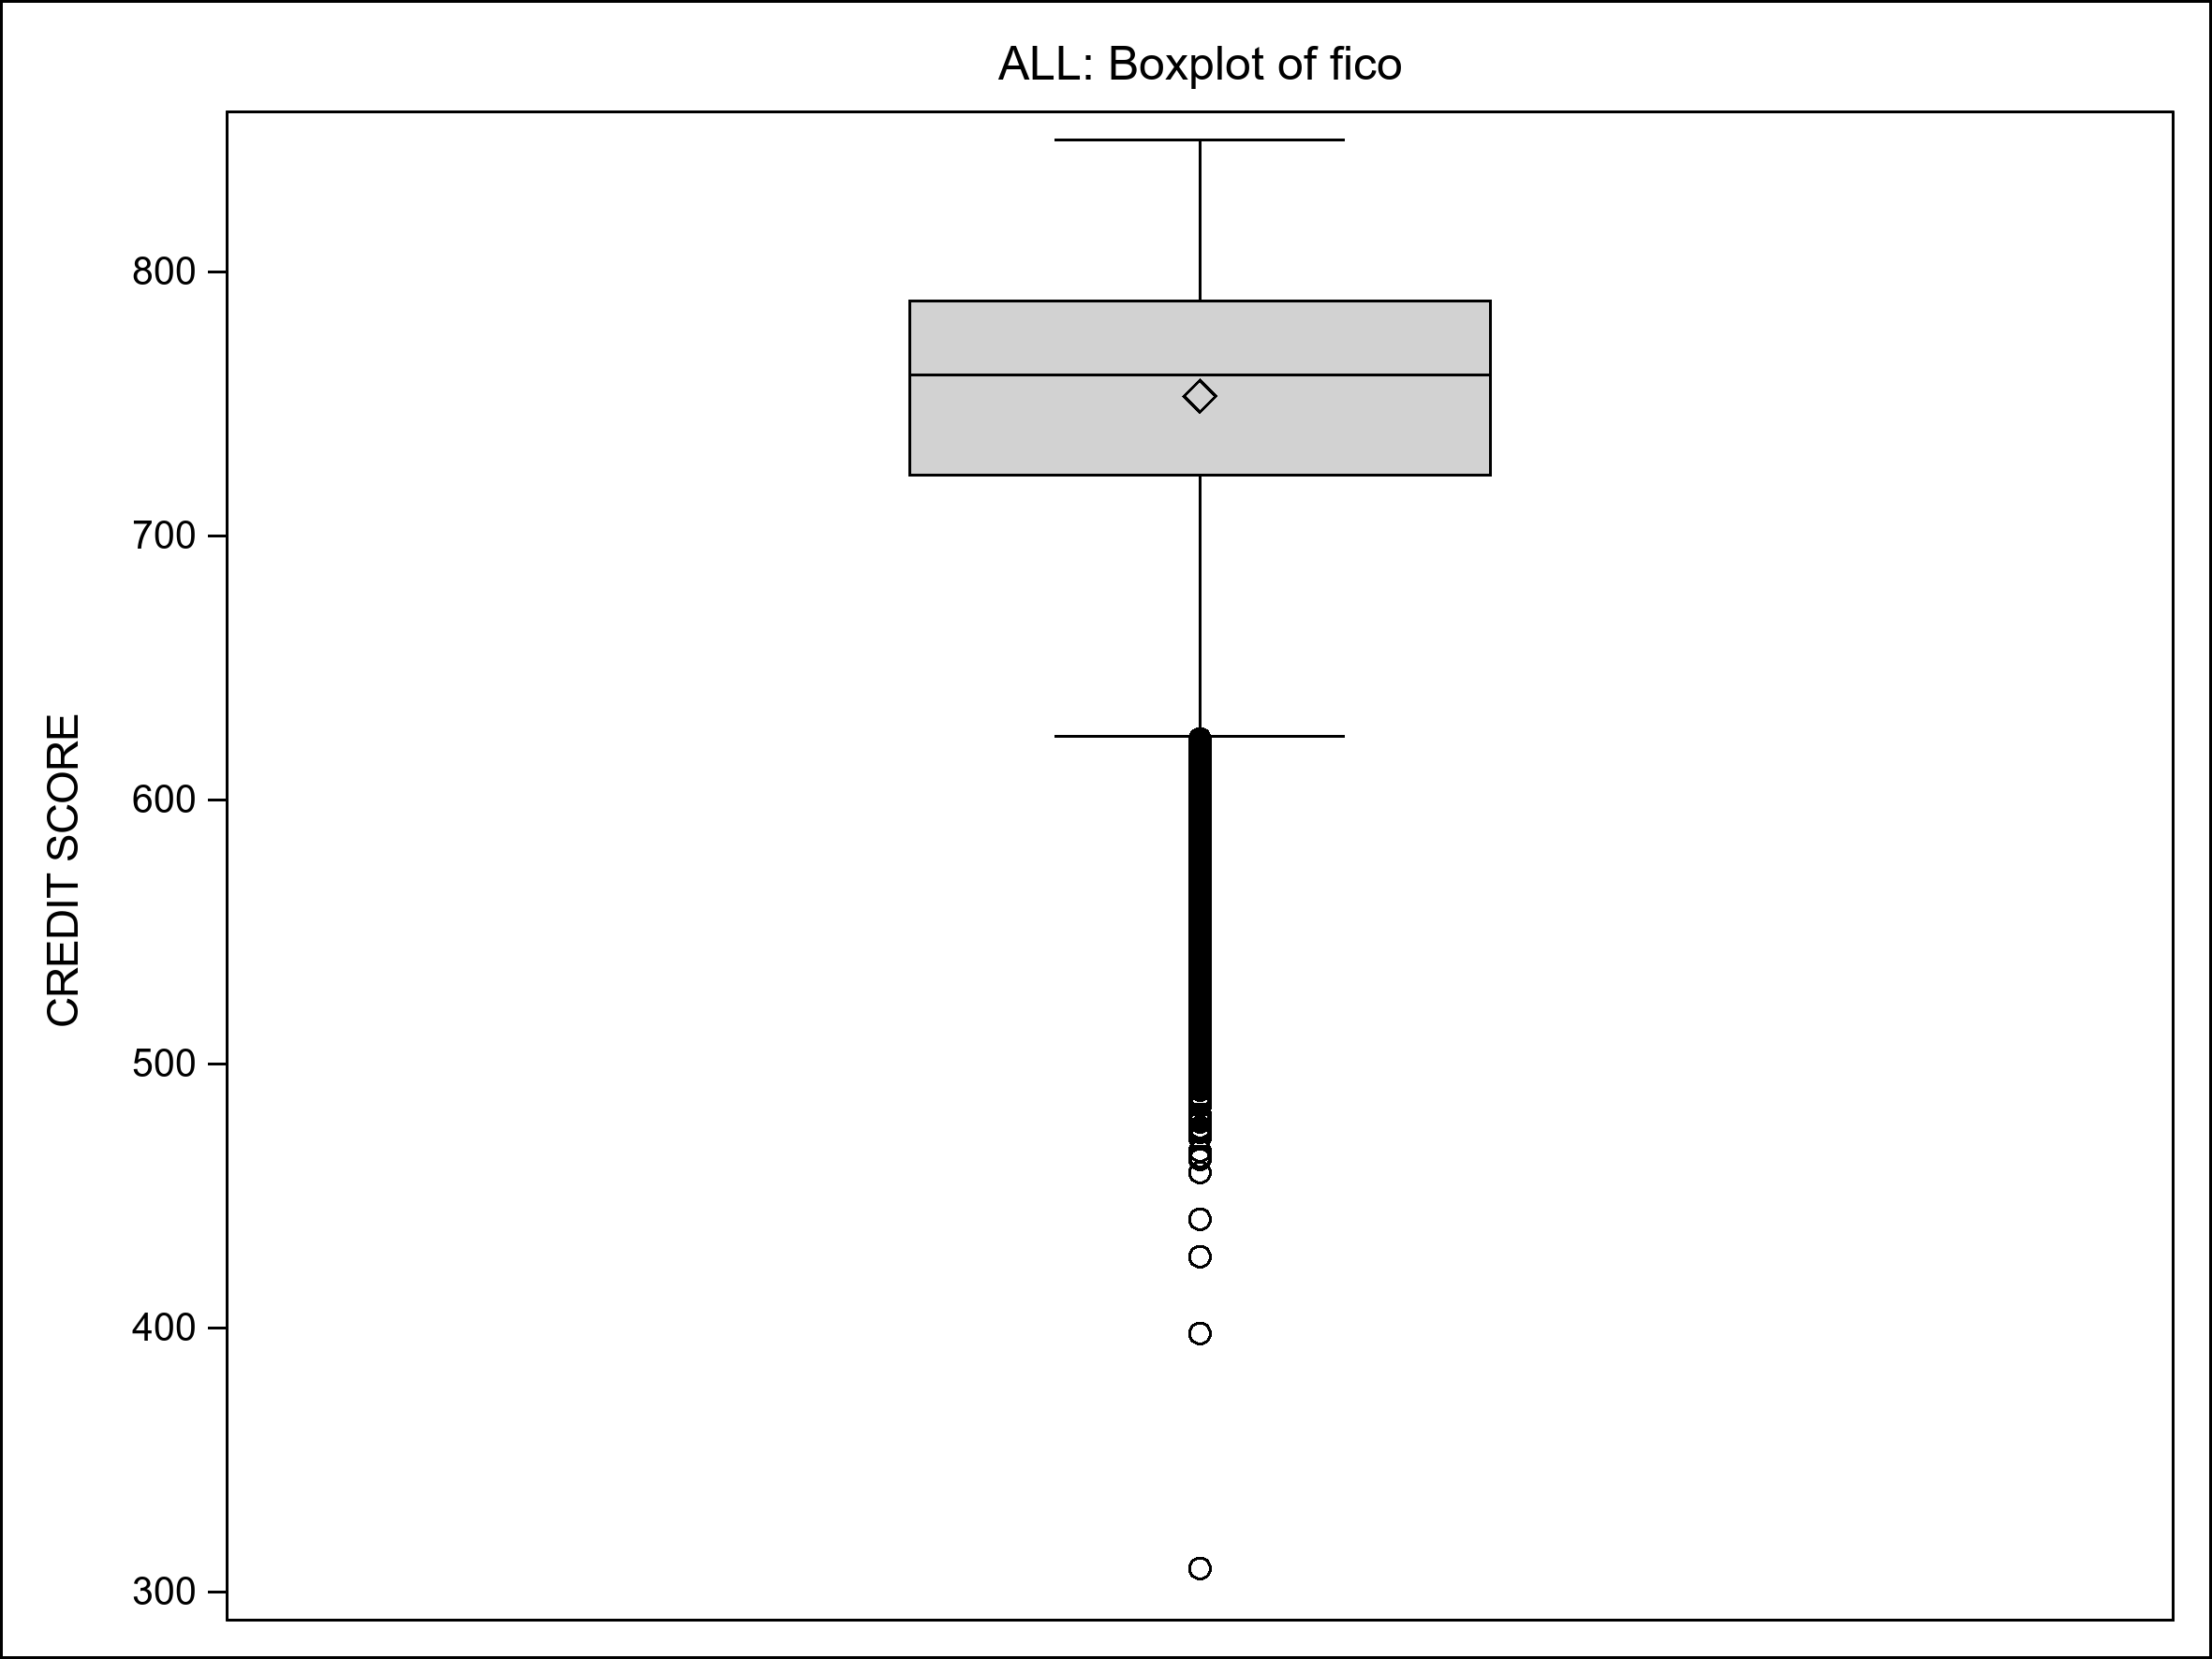
\includegraphics[width=0.9\textwidth]{./plot/Boxplot/Main/NUM_fico_BOXPLOT_ALL1.png}
\end{minipage}%
\begin{minipage}{.5\textwidth}
	\centering
	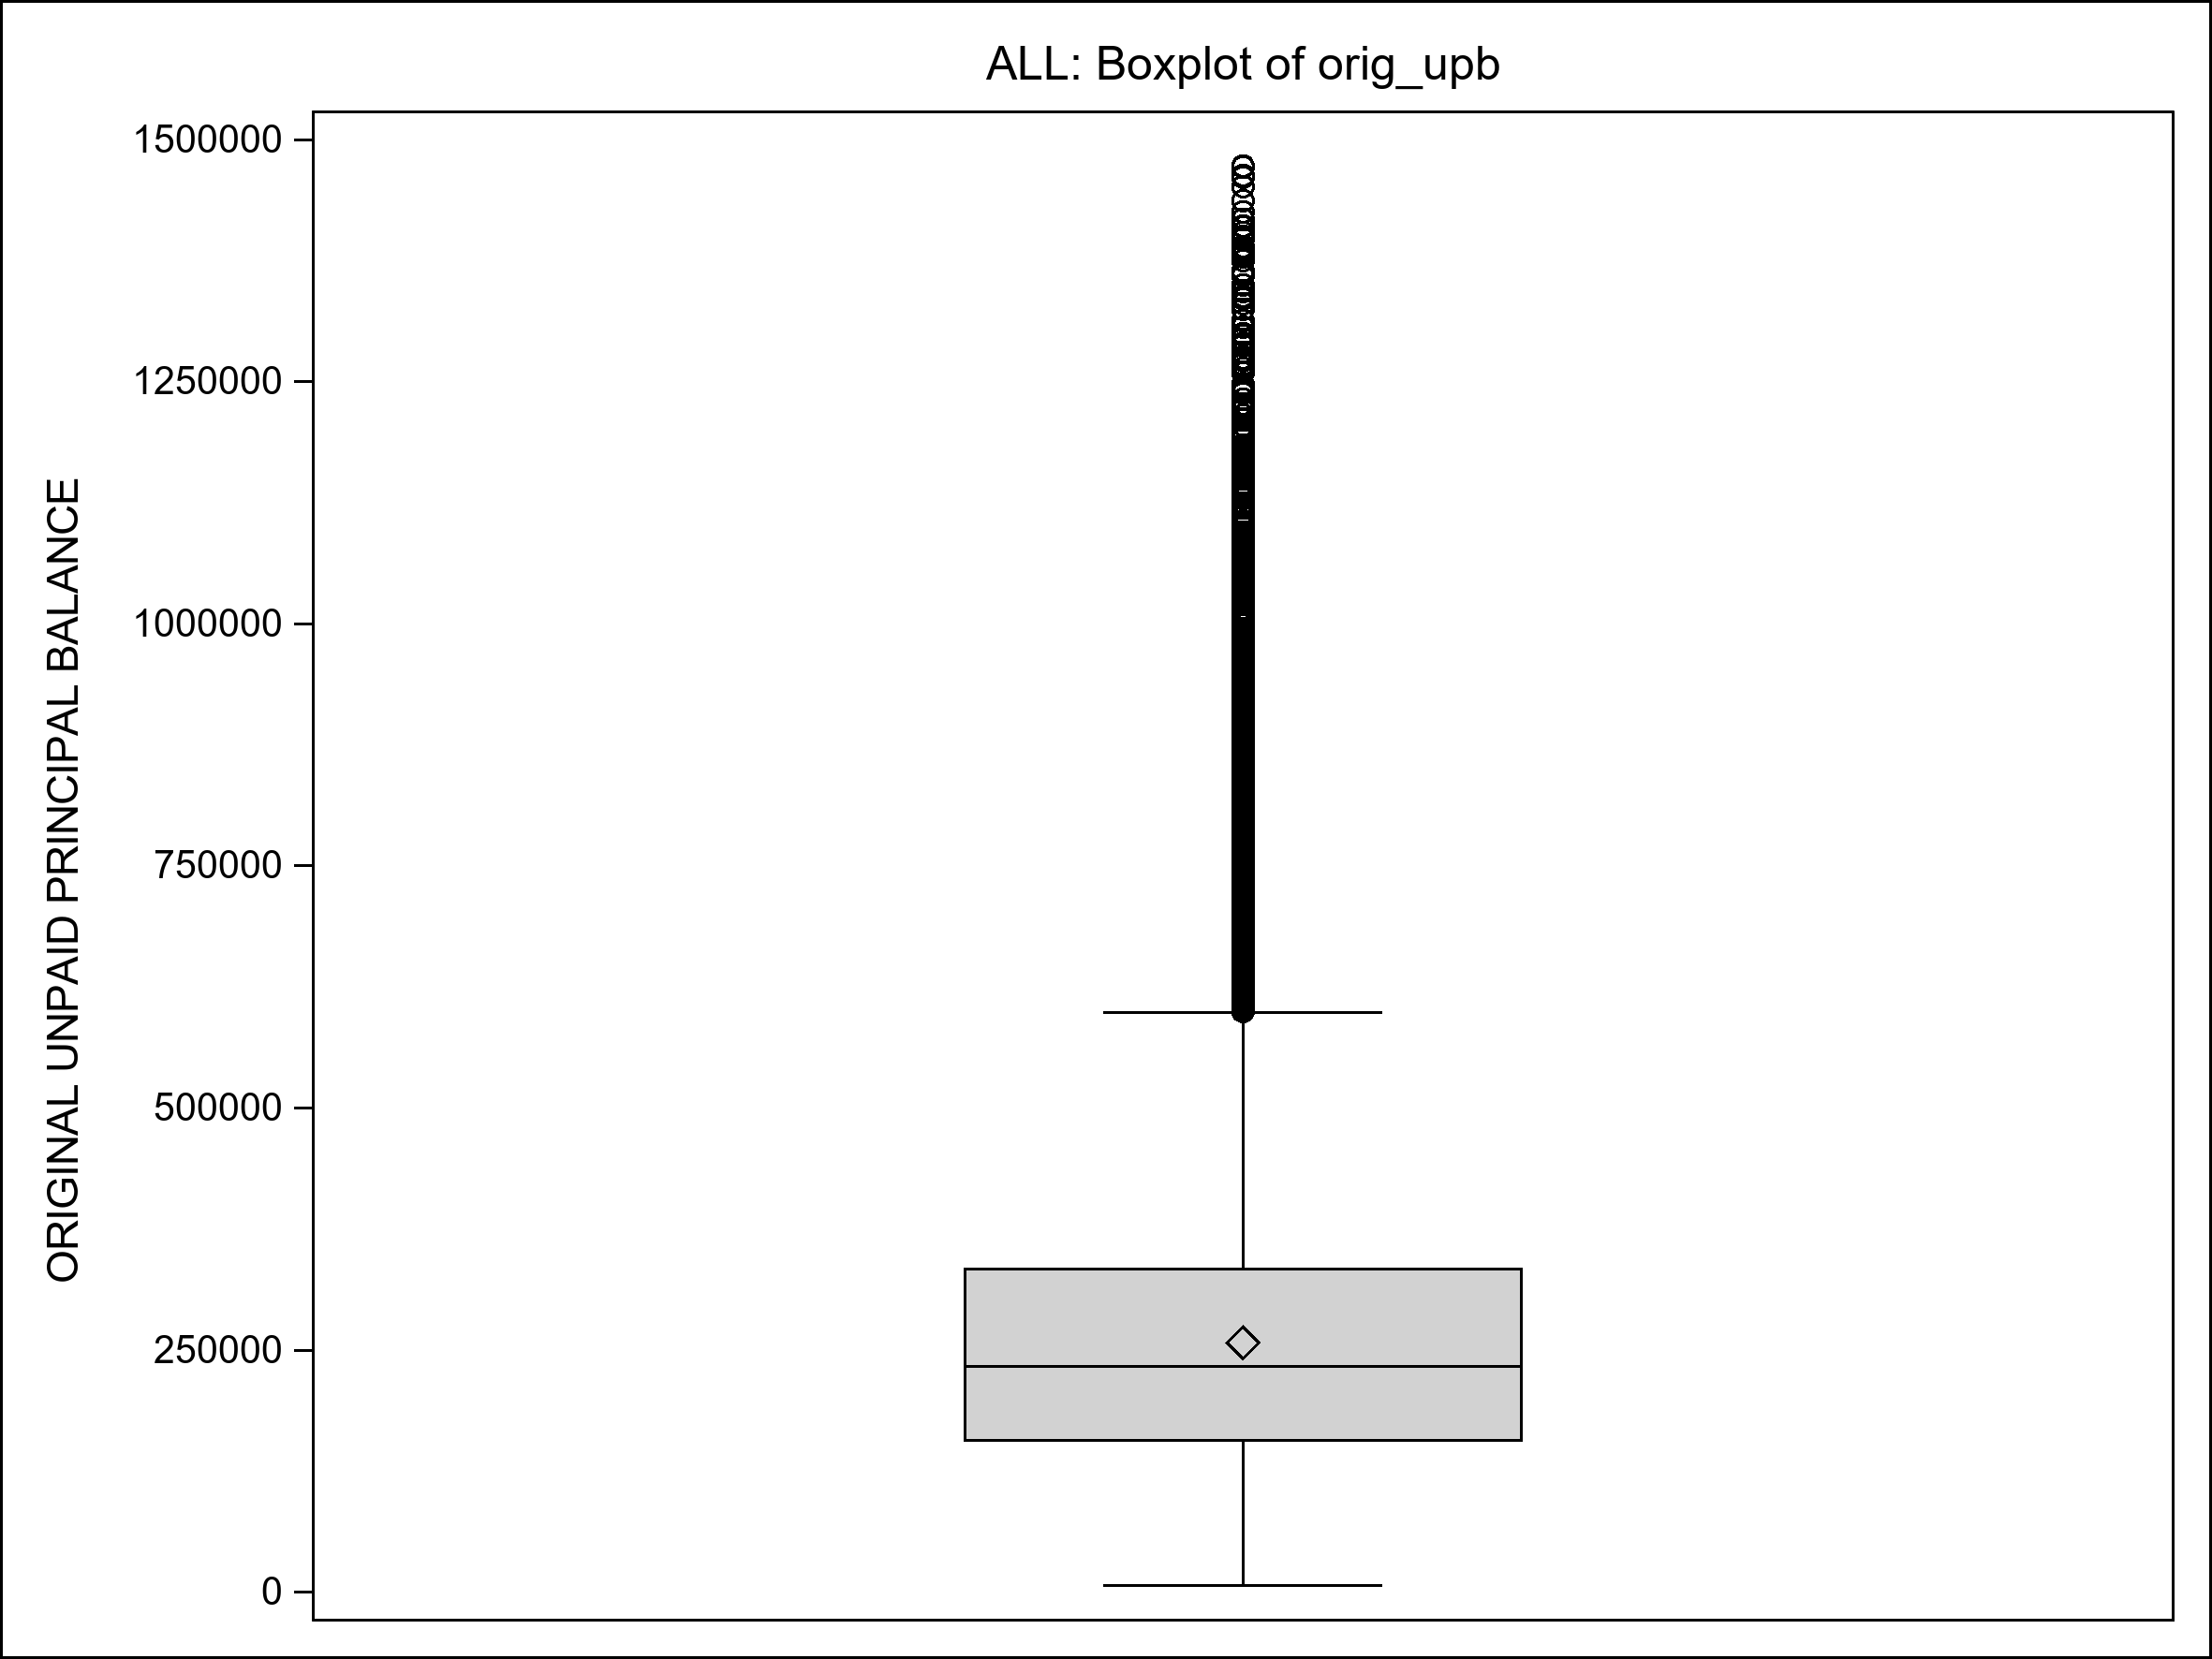
\includegraphics[width=0.9\textwidth]{./plot/Boxplot/Main/NUM_orig_upb_BOXPLOT_ALL1.png}
\end{minipage}
    \caption{Boxplot of Credit Score (fico) and Original UPB}
    \label{fig:re_boxpl_fico_origupb}
\end{figure}
\begin{figure}[H]
\begin{minipage}{.5\textwidth}
	\centering
	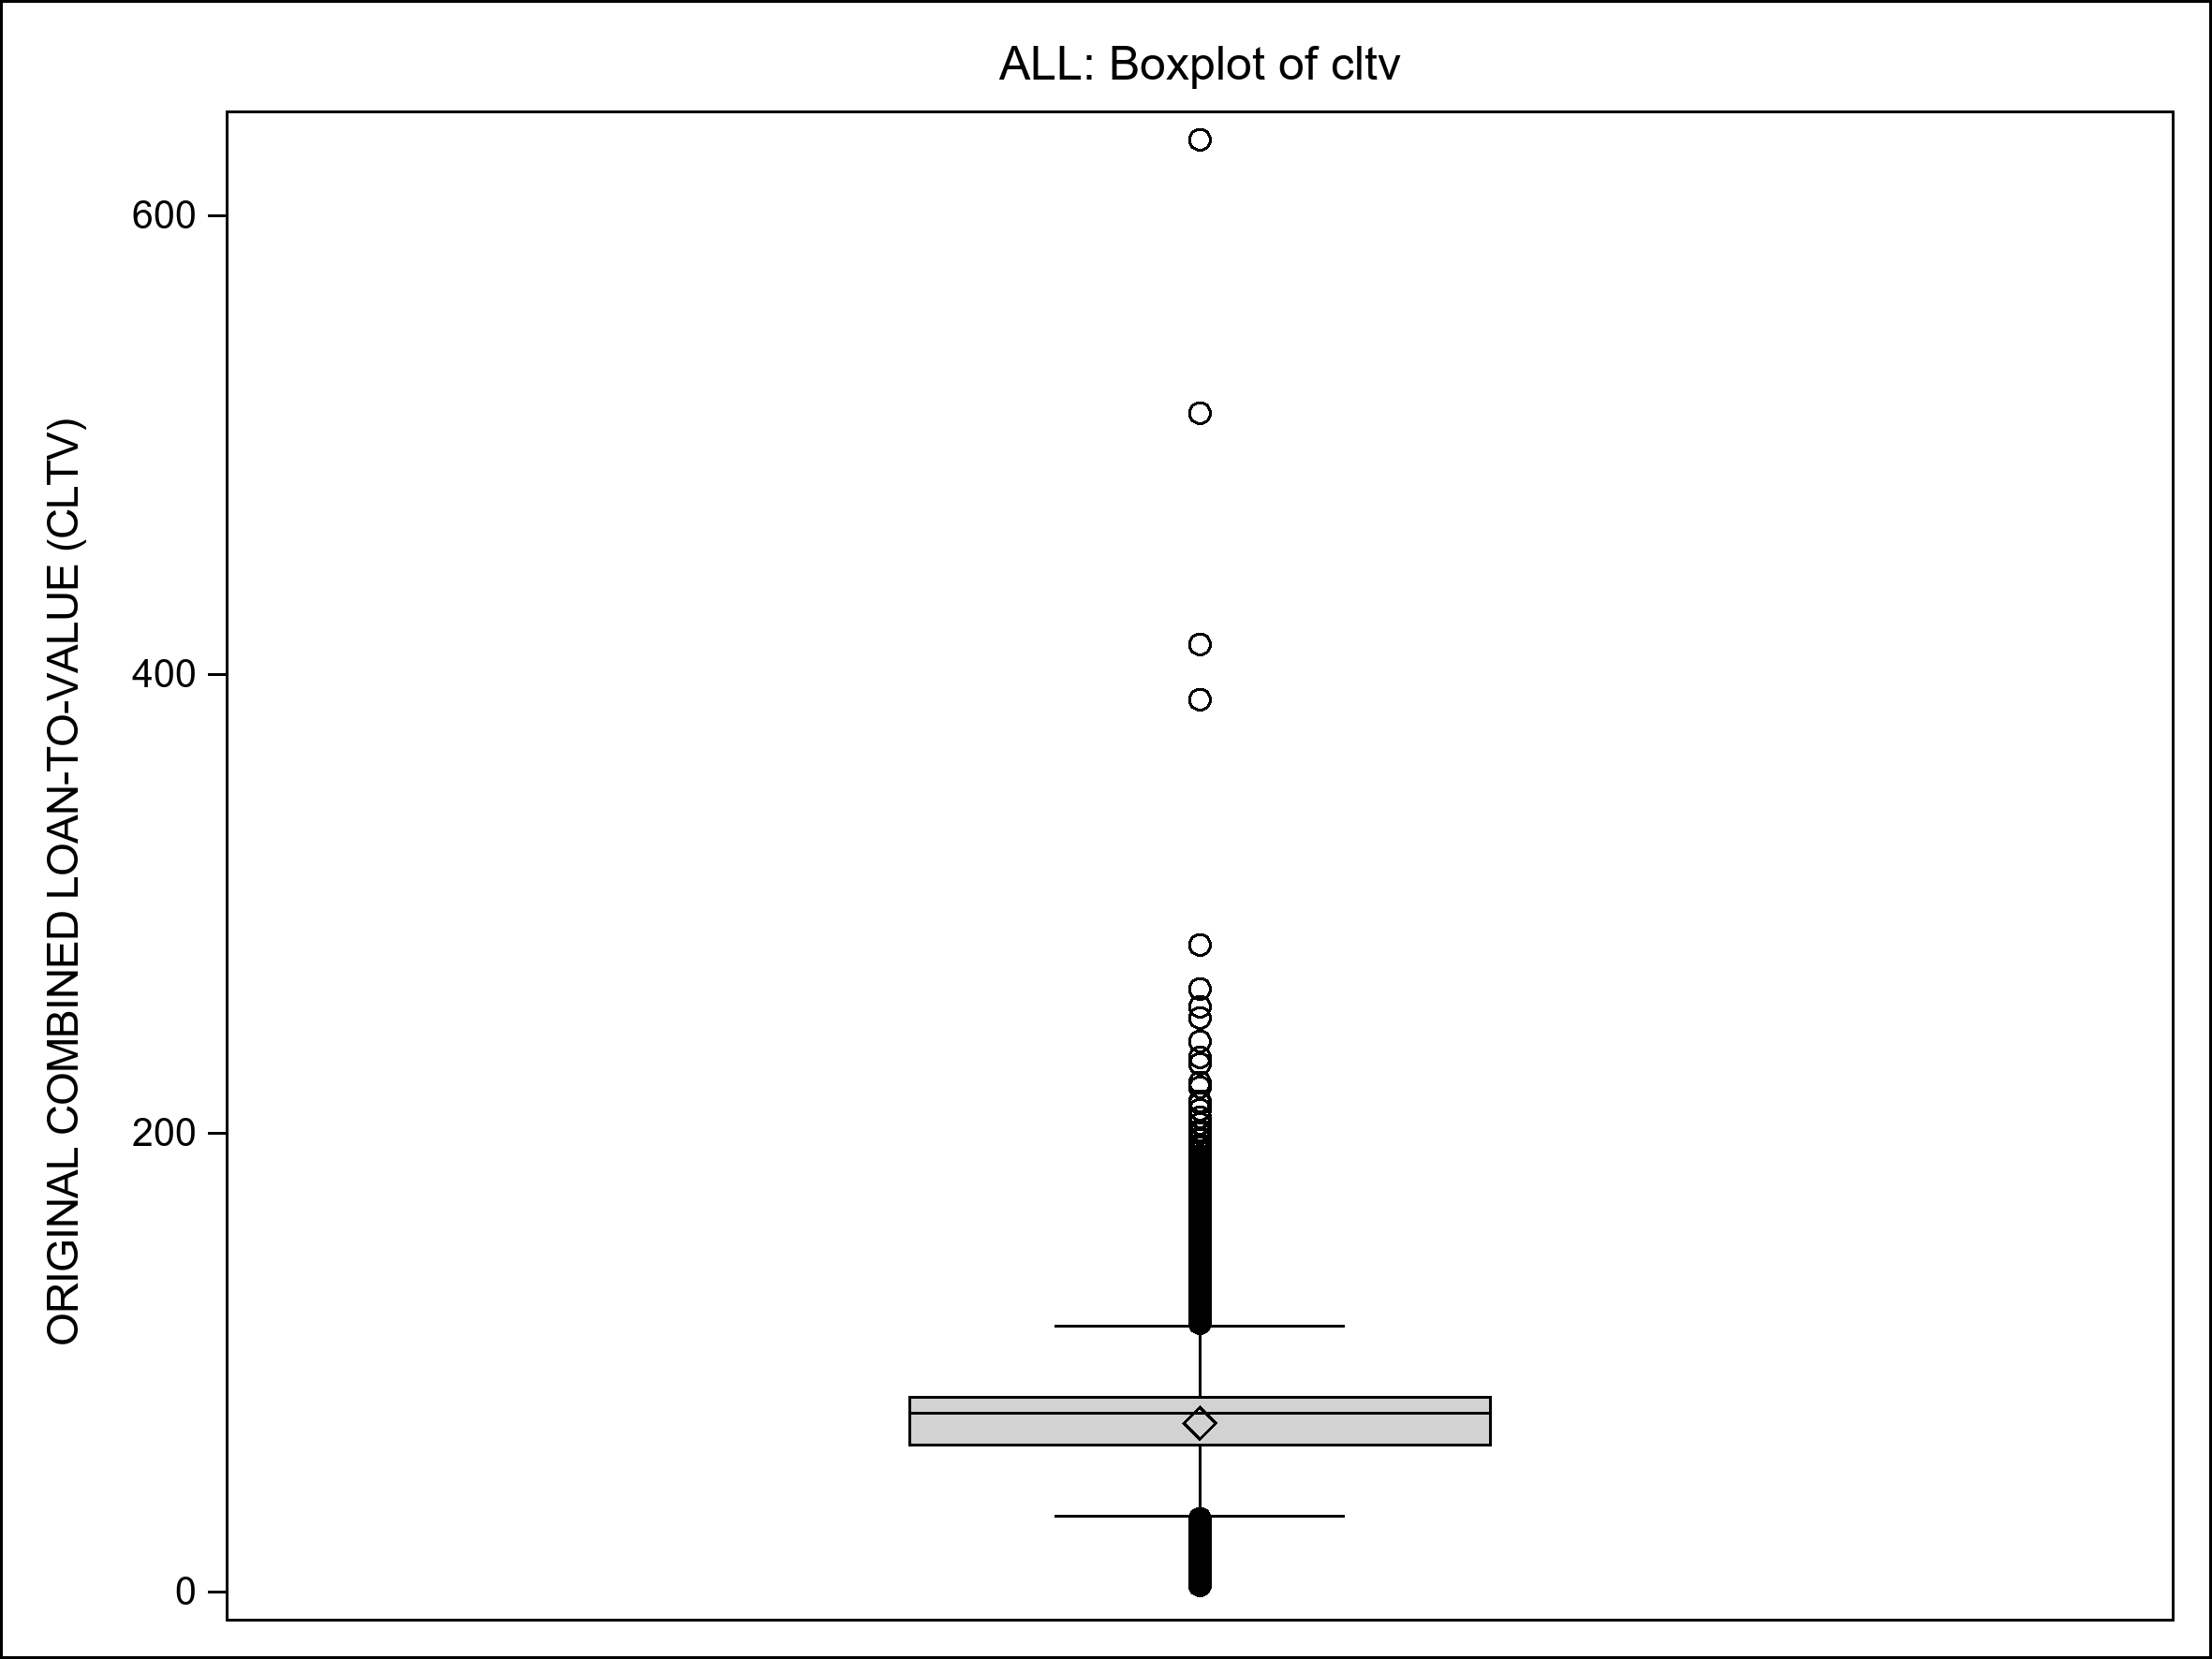
\includegraphics[width=0.9\textwidth]{./plot/Boxplot/Main/NUM_cltv_BOXPLOT_ALL1.png}
\end{minipage}%
\begin{minipage}{.5\textwidth}
	\centering
	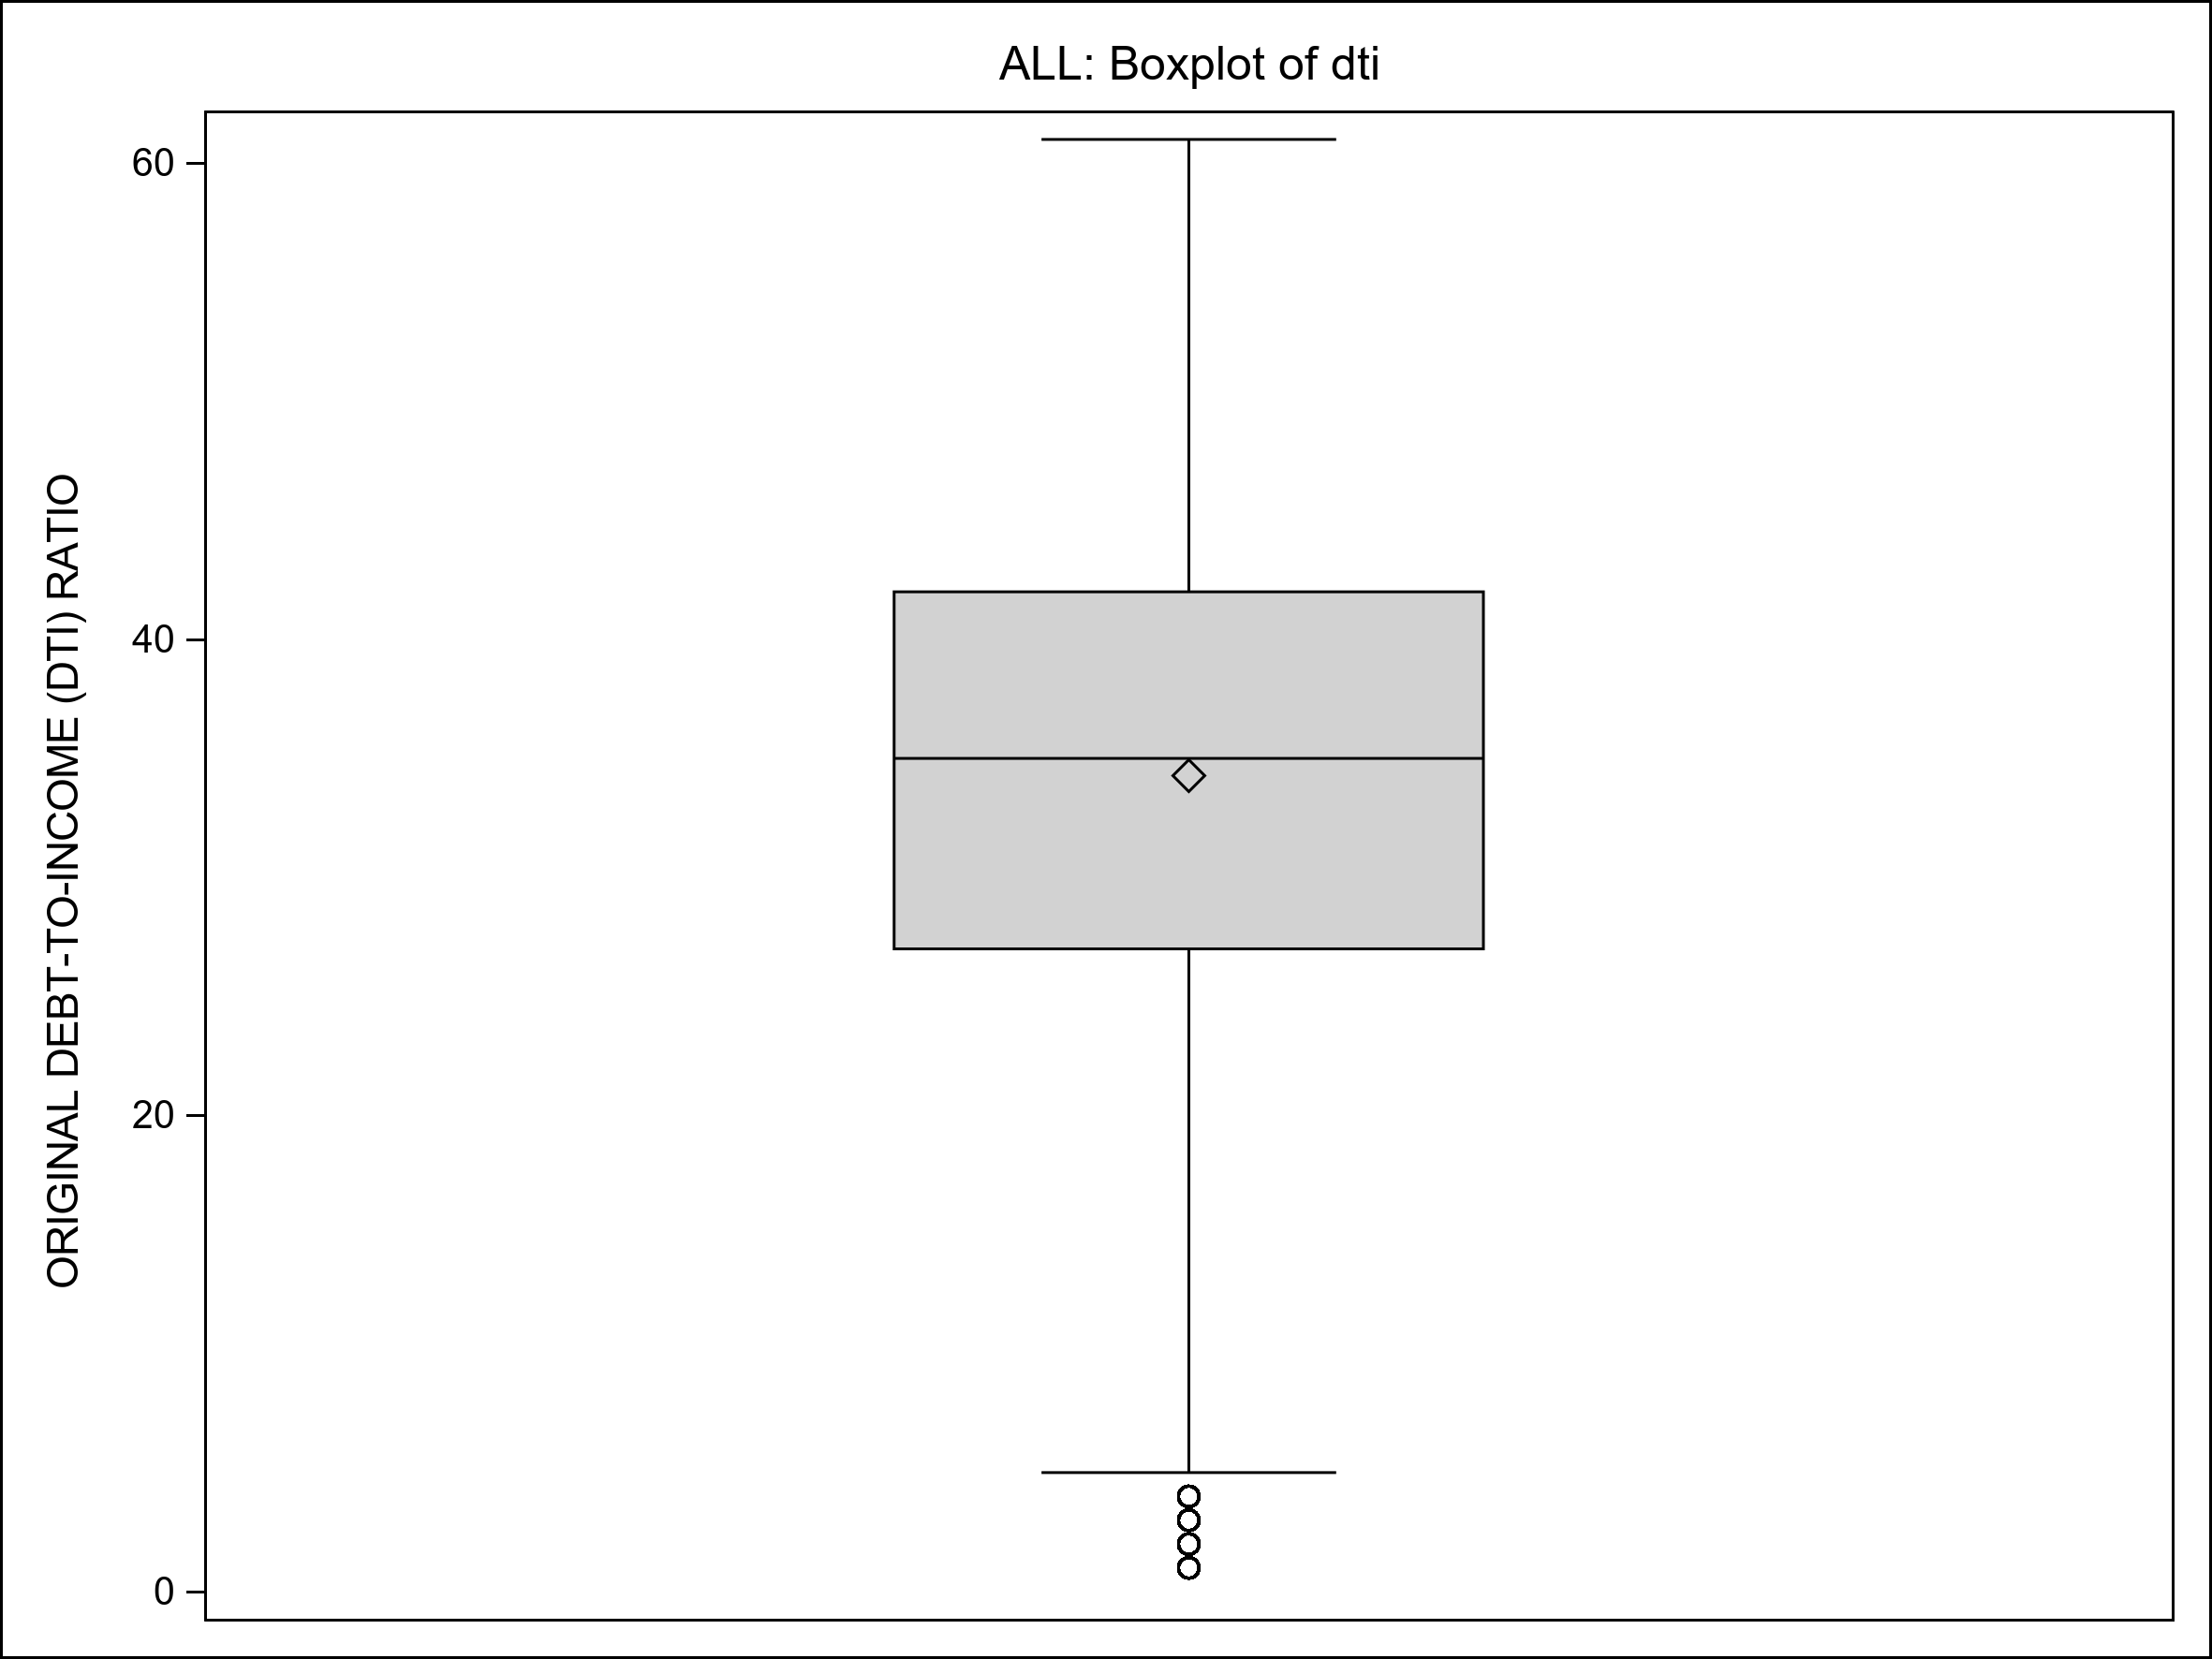
\includegraphics[width=0.9\textwidth]{./plot/Boxplot/Main/NUM_dti_BOXPLOT_ALL1.png}
\end{minipage}
    \caption{Boxplot of CLTV and DTI}
    %\label{fig:dp_iqr_boxpl}
\end{figure}
\begin{figure}[H]
\begin{minipage}{.5\textwidth}
	\centering
	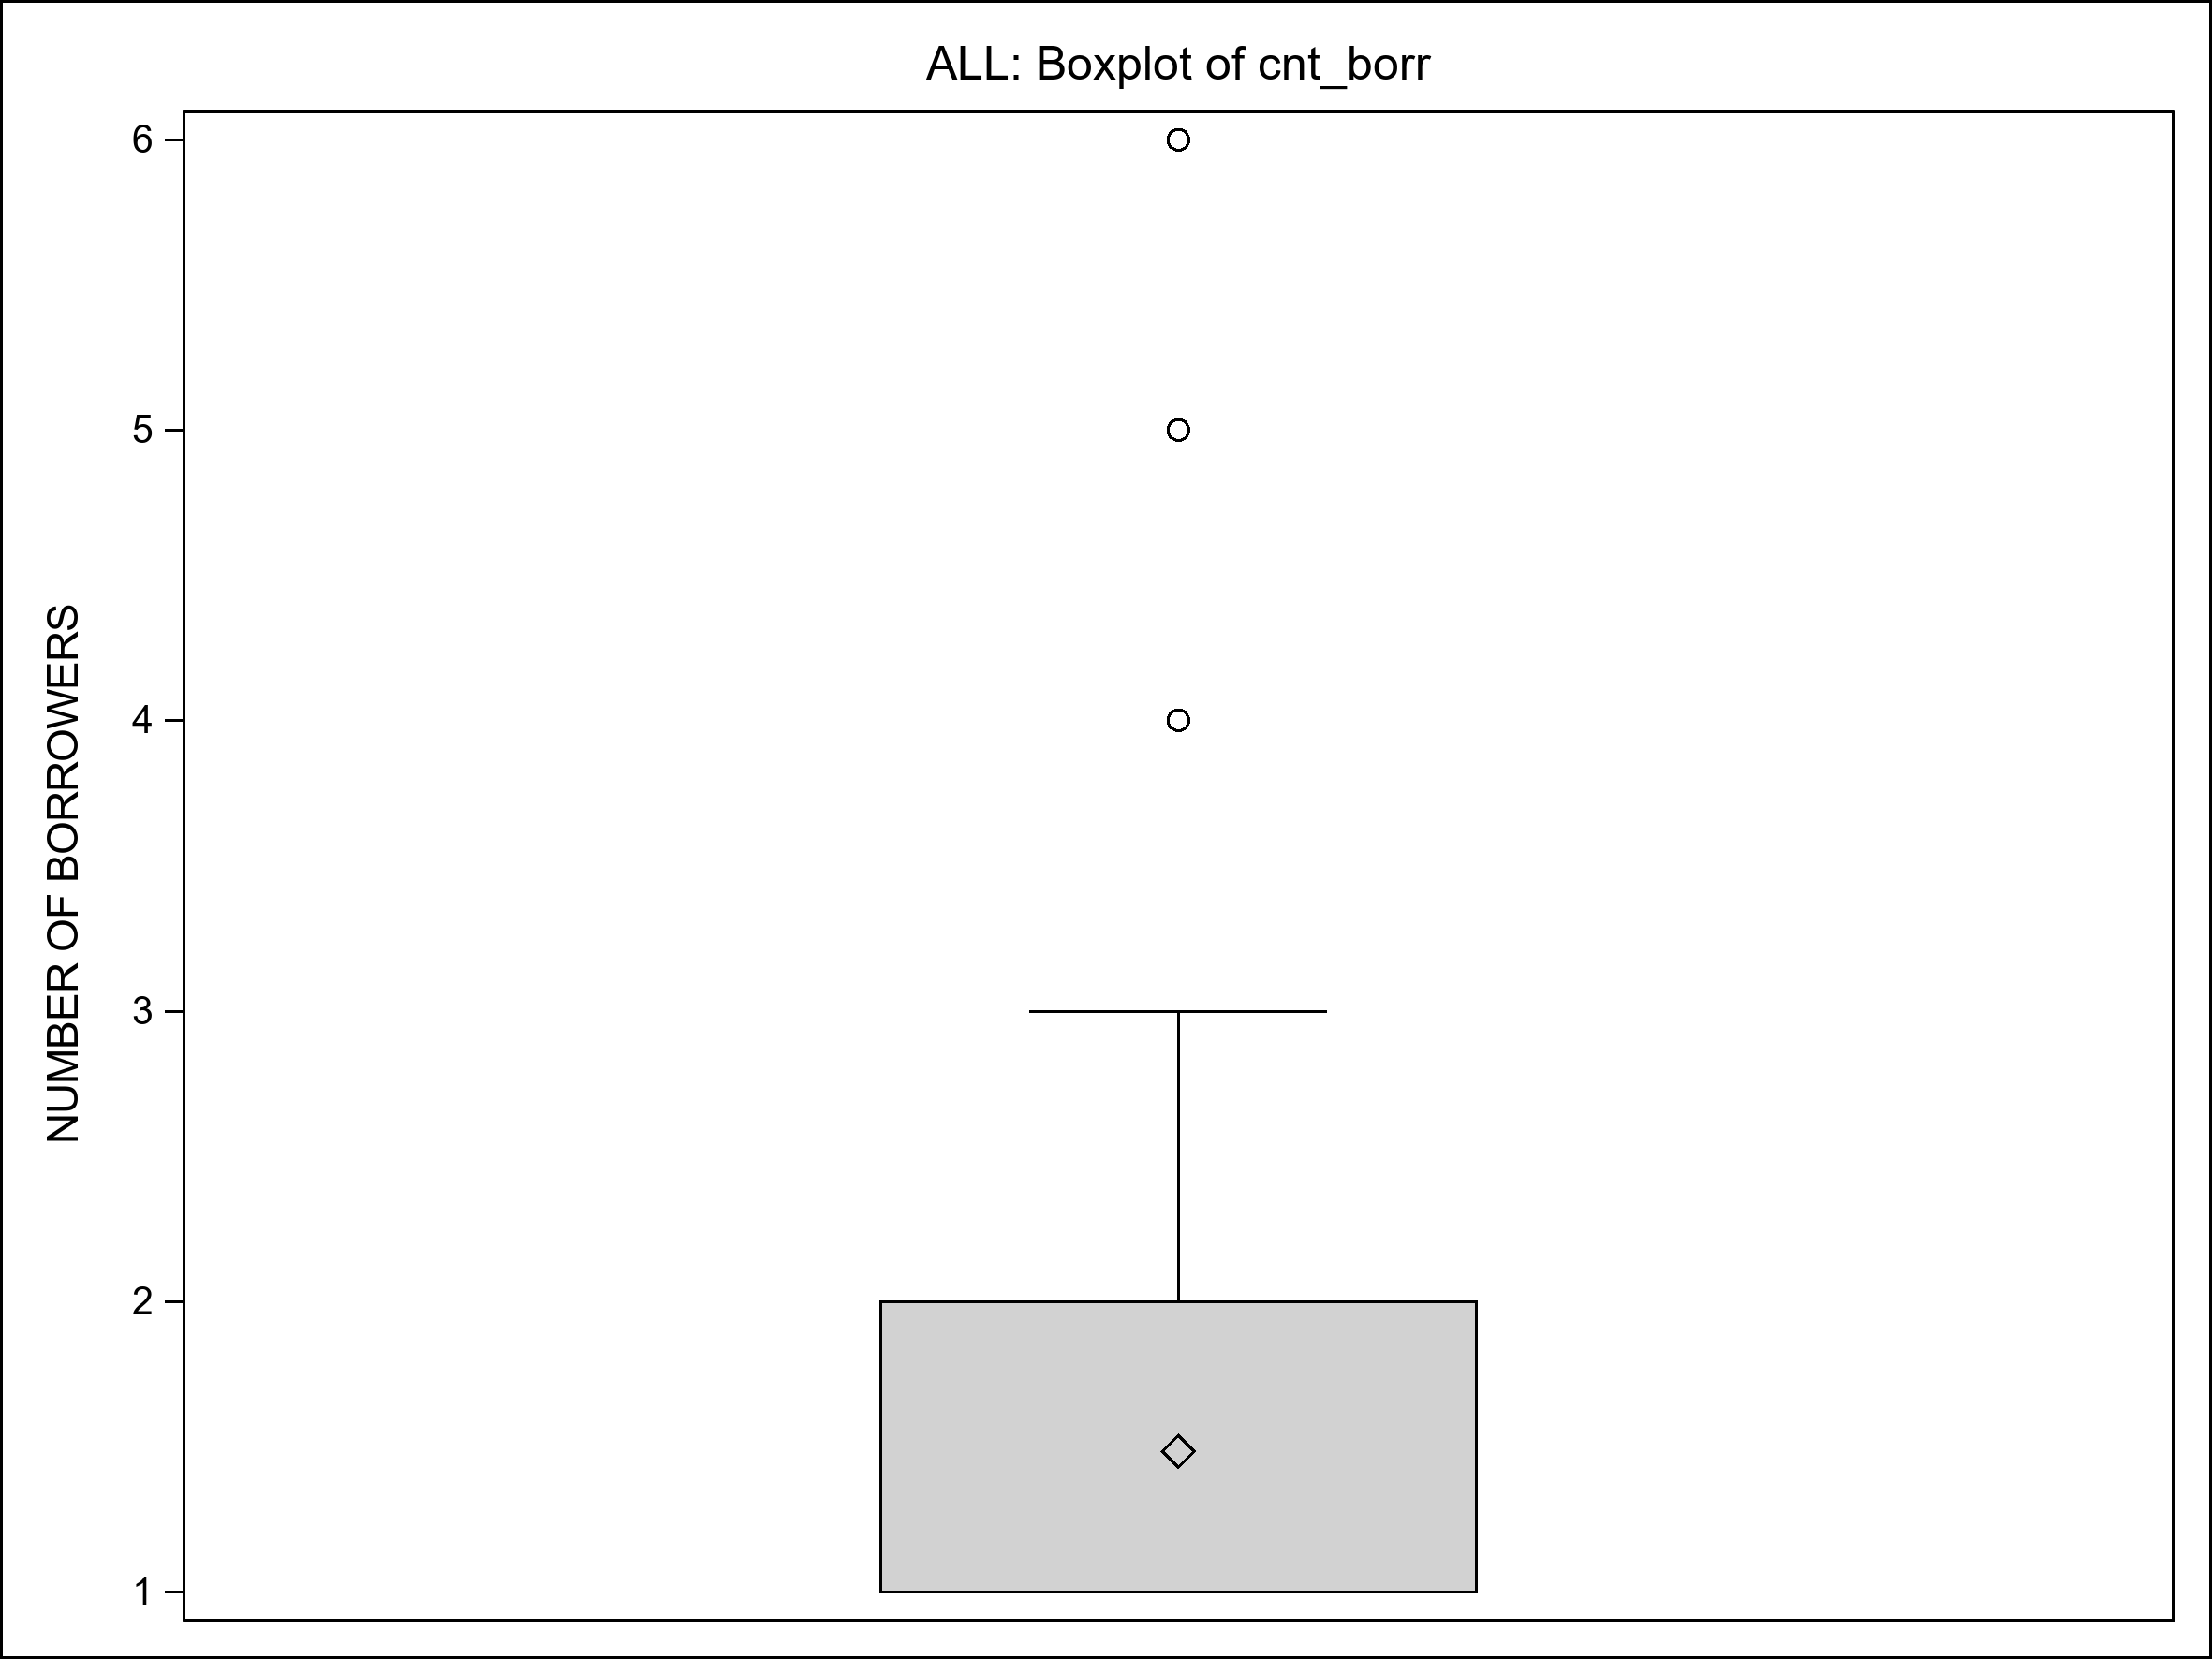
\includegraphics[width=0.9\textwidth]{./plot/Boxplot/Main/NUM_cnt_borr_BOXPLOT_ALL1.png}
\end{minipage}%
\begin{minipage}{.5\textwidth}
	\centering
	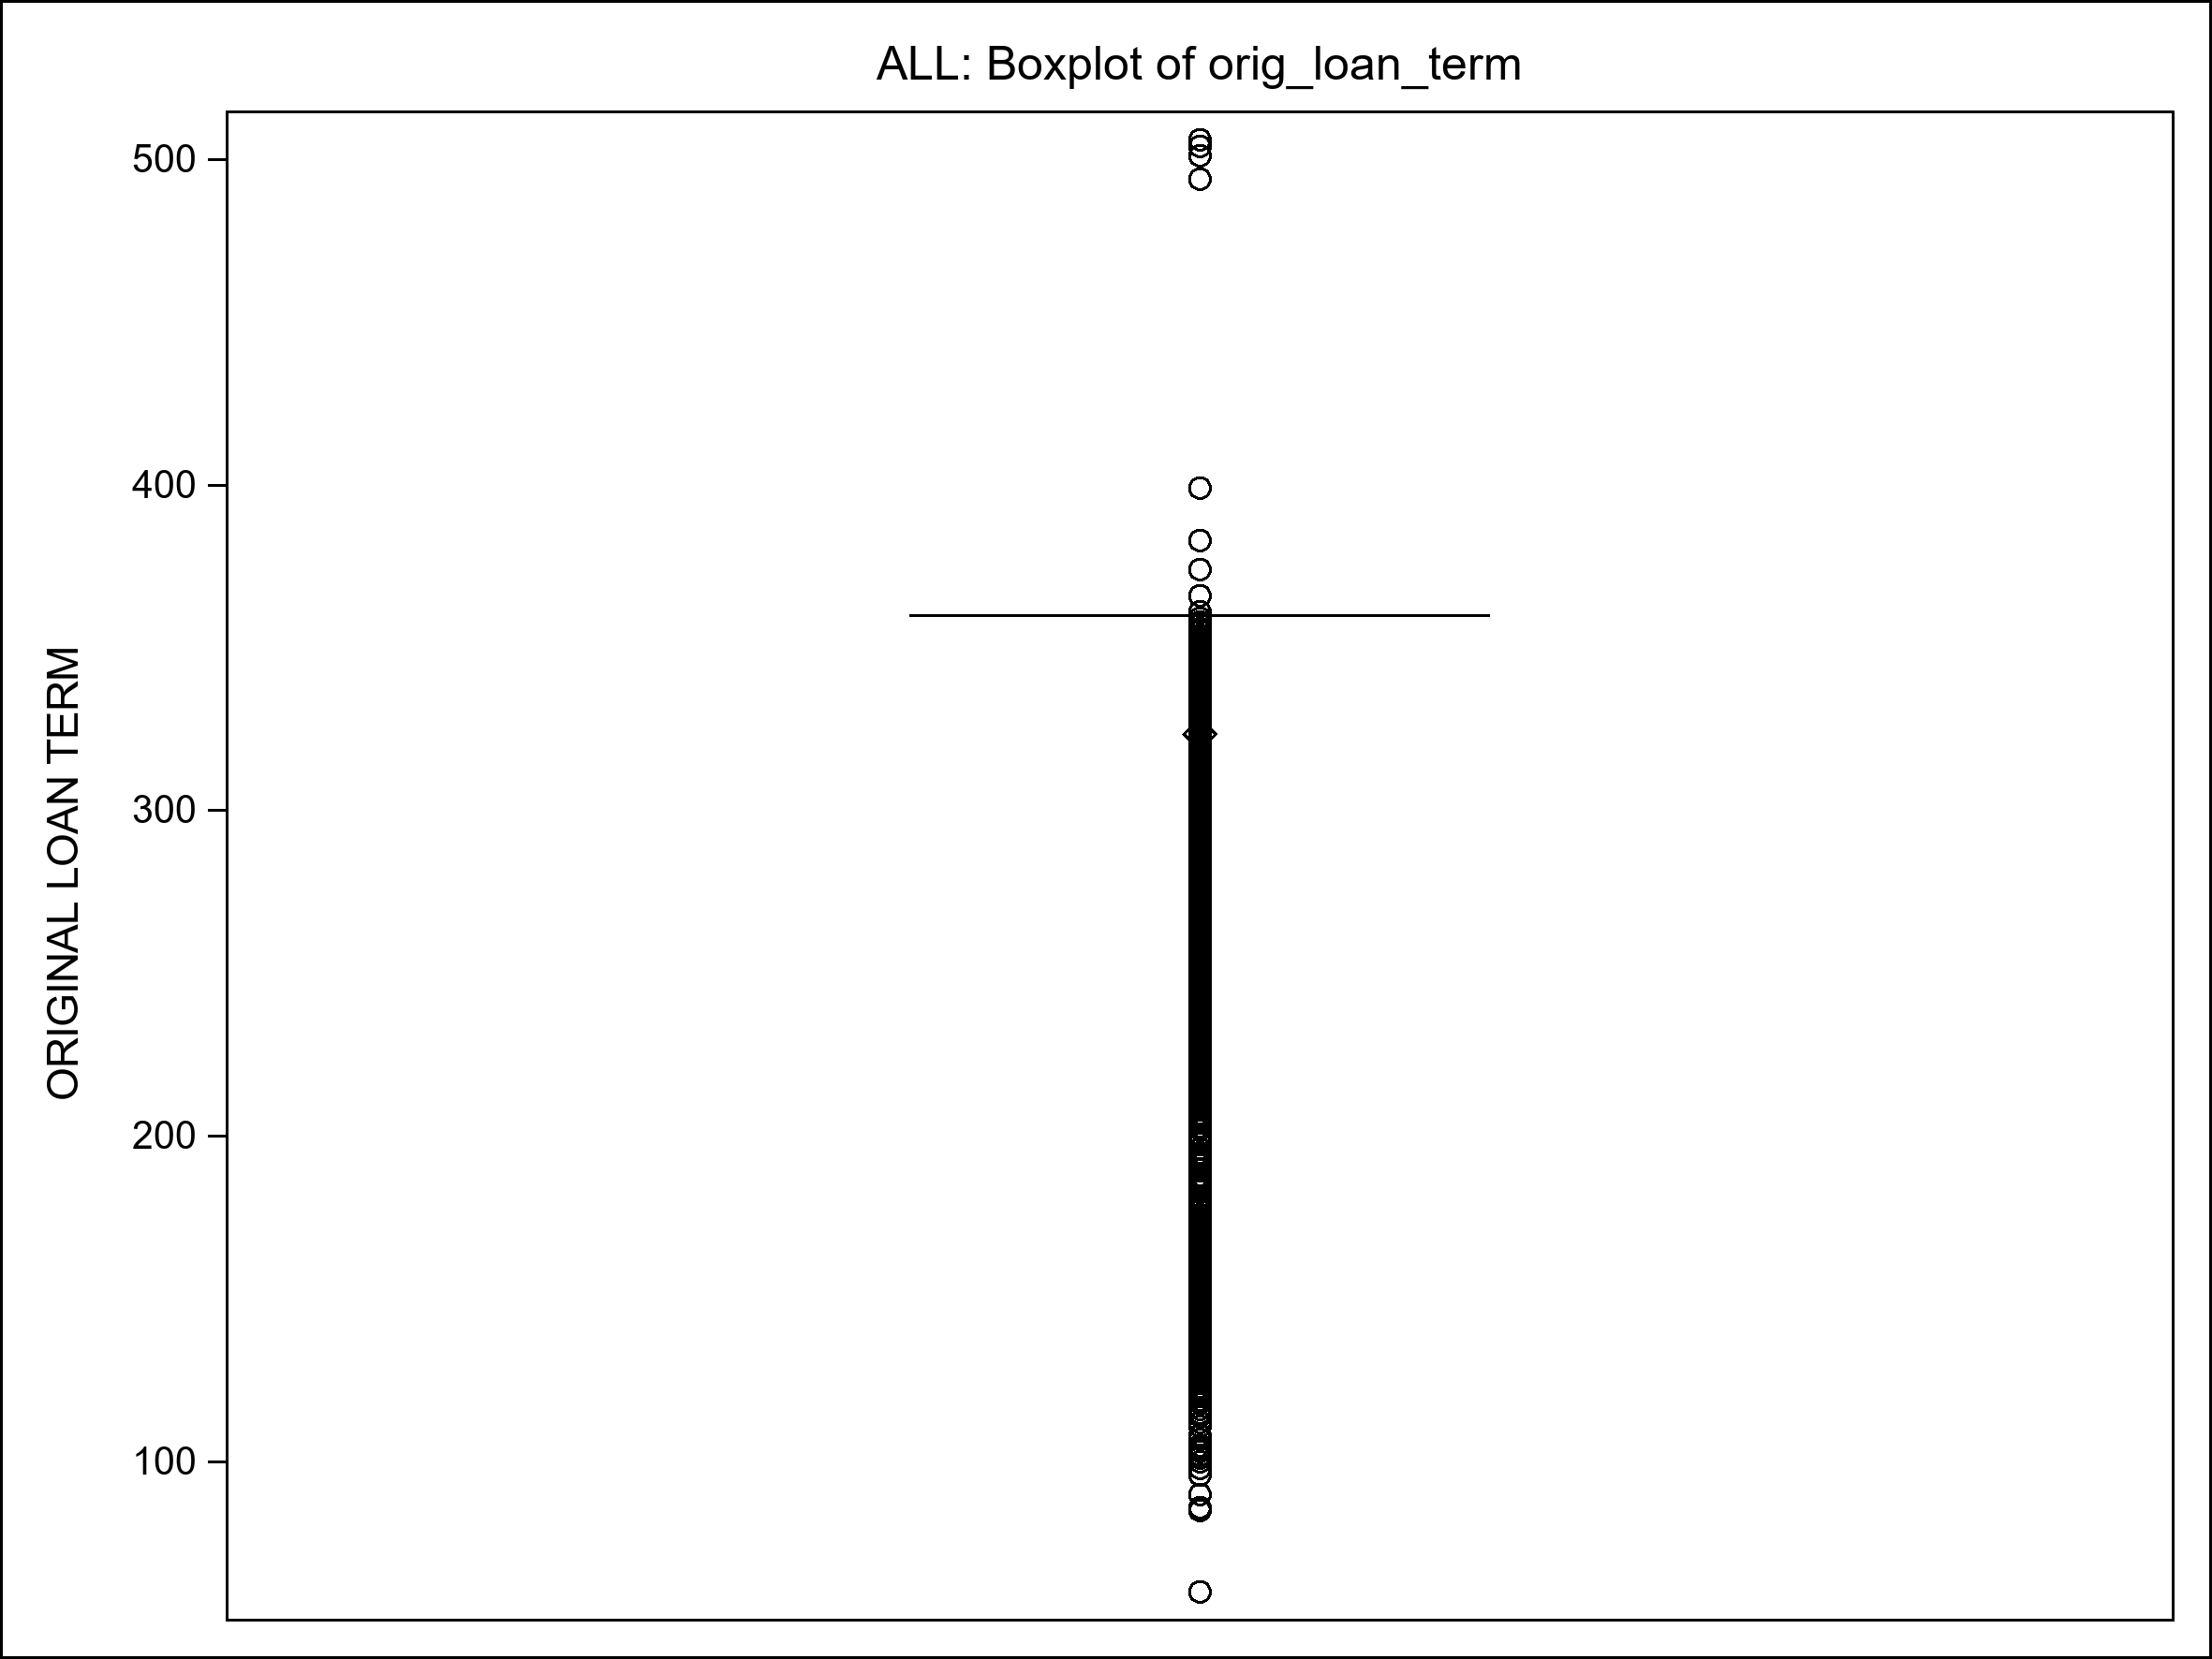
\includegraphics[width=0.9\textwidth]{./plot/Boxplot/Main/NUM_orig_loan_term_BOXPLOT_ALL1.png}
\end{minipage}
    \caption{Boxplot of Numner of Borrowers and Original Loan Term}
    \label{fig:re_boxpl_noborr_loanterm}
\end{figure}


% Please add the following required packages to your document preamble:
% \usepackage{graphicx}
% \usepackage{lscape}
\begin{landscape}

\begin{table}[]
\centering
\resizebox{1.3\textwidth}{!}{%
\begin{tabular}{llllllllllllll}\toprule
\textbf{Variable}     & \textbf{Sum}               & \textbf{Mean}    & \textbf{Mode}    & \textbf{StdDev}  & \textbf{Min}   & \textbf{P1}     & \textbf{P5}     & \textbf{P25}     & \textbf{Median}  & \textbf{P75}     & \textbf{P95}     & \textbf{P99}     & \textbf{Max}       \\\midrule
CLTV         & 398.545.357       & 73,62     & 80      & 17,27     & 3     & 25     & 39     & 64      & 78      & 85      & 95      & 97      & 633       \\
No Borrowers & 8.030.443         & 1,48      & 1       & 0,52      & 1     & 1      & 1      & 1       & 1       & 2       & 2       & 2       & 6         \\
No Units     & 5.566.001         & 1,03      & 1       & 0,22      & 1     & 1      & 1      & 1       & 1       & 1       & 1       & 2       & 4         \\
DTI          & 184.916.404       & 34,28     & 45      & 9,70      & 1     & 12     & 17     & 27      & 35      & 42      & 48      & 50      & 61        \\
Credit Score & 4.074.892.728     & 752,92    & 801     & 43,93     & 309   & 637    & 670    & 723     & 761     & 789     & 809     & 817     & 850       \\
LTV          & 397.336.584       & 73,40     & 80      & 17,29     & 3     & 24     & 39     & 64      & 77      & 85      & 95      & 97      & 514       \\
MI Perc      & 37.410.176        & 6,91      & 0       & 11,56     & 0     & 0      & 0      & 0       & 0       & 12      & 30      & 30      & 52        \\
Loan Term    & 1.751.503.811     & 323,53    & 360     & 69,96     & 60    & 180    & 180    & 360     & 360     & 360     & 360     & 360     & 506       \\
UPB          & 1.390.864.618.000 & 256916,67 & 200.000 & 131963,97 & 7.000 & 54.000 & 85.000 & 157.000 & 233.000 & 334.000 & 502.000 & 663.000 & 1.473.000 \\\bottomrule
\end{tabular}%
}
\caption{Descriptive statistics}
\label{tab:re_descr_stat}
\end{table}

\begin{table}[]
\centering
\resizebox{1.3\textwidth}{!}{%
\begin{tabular}{lrrrrrrrr}\toprule
\textbf{Variable} & \textbf{Lower Boarder}     & \textbf{Upper Boarder} & \textbf{\# below Lower Boarder} & \textbf{\# above Upper Boarder} & \textbf{\% below Lower Boarder} & \textbf{\% above Upper Boarder} & \textbf{\# Outliers} & \textbf{\% Outliers} \\\midrule
CLTV         & 32,5    & 116,5  & 142518  & 596    & 2,63\%  & 0,01\% & 143.114   & 2,64\%  \\
No Borrowers & -0,5    & 3,5    & 0       & 5461   & 0,00\%  & 0,10\% & 5.461     & 0,10\%  \\
No Units     & 1       & 1      & 0       & 108940 & 0,00\%  & 2,01\% & 108.940   & 2,01\%  \\
DTI          & 4,5     & 64,5   & 21294   & 0      & 0,39\%  & 0,00\% & 21.294    & 0,39\%  \\
Credit Score & 624     & 888    & 16444   & 0      & 0,30\%  & 0,00\% & 16.444    & 0,30\%  \\
LTV          & 32,5    & 116,5  & 145323  & 394    & 2,68\%  & 0,01\% & 145.717   & 2,69\%  \\
MI Perc      & -18     & 30     & 19      & 25853  & 0,00\%  & 0,48\% & 25.872    & 0,48\%  \\
Loan Term    & 360     & 360    & 1236041 & 18     & 22,83\% & 0,00\% & 1.236.059 & 22,83\% \\
UPB          & -108500 & 599500 & 0       & 102141 & 0,00\%  & 1,89\% & 102.141   & 1,89\%   \\\bottomrule                                
\end{tabular}%
}
\caption{Interquartile range}
\label{tab:re_iqr}
\end{table}

\end{landscape}

\section{Variable Selection}
\subsection{Univariate Analysis}

\subsubsection{New variables}
During the outlier treatment, a few new variables were created. While analyzing the different distinct values of categorical variables, the risk factor \emph{Property states} was grouped into five \emph{US regions} according to their geographical position: Northeast, Southeast, Southwest, Midwest, West and other Regions, e.g., outside of the North American mainland. Table \ref{tab:re_descr_newvar} lists a summary of the new variables.

\begin{table}[H]
\centering
\begin{tabular}{ Lp{8cm}R } \toprule
\textbf{Variable Name}  & \textbf{Description}                                                                                                                                                                                                                                                          & \textbf{Abbr.}       \\\midrule
MI Percentage Indicator                                        & Indicator, that Mortgage Insurance Percentage \textgreater 0\%                           & MI Flag                     \\\hline
Loan Term \textgreater 360 Months                              & Indicator, that Original Loan Term \textgreater 360 Months                               & Loan Term \textgreater 360m \\\hline
Loan Term Group                                                & Grouped Variable, Original Loan Term is "\textless 360m", "= 360m", "\textgreater{}360m" & Loan Term Group             \\\hline
Loan Term $\geq$ 360 Months Indicator                          & Indicator, that Original Loan Term $\geq$ 360 Months                                     & Loan Term $\geq$ 360m        \\\hline
Indicator, that Original Loan Term = 360 Months                & Indicator, that Original Loan Term = 360 Months                                          & Loan Term = 360m            \\\hline
Original Combined Loan-to-Value (CLTV) after Outlier Treatment & Original Combined Loan-to-Value (CLTV) after Outlier Treatment                           & CLTV adj                    \\\hline
Original Loan-to-Value (LTV) after Outlier Treatment           & Original Loan-to-Value (LTV) after Outlier Treatment                                     & LTV adj                     \\\hline
US Region                                                      & Grouped variable of "Property State"                                                     & US Region                \\\bottomrule
\end{tabular}%
\caption{Description of new variables}
\label{tab:re_descr_newvar}
\end{table}

\subsubsection{Discriminatory Power}
To assess the discriminatory power, distribution plots with default rates, ROC curves and calculations of AUC, GINI coefficients, WoE and IV were conducted. A list of all metrics is presented in Table \ref{tab:re_discr_power} and relevant variable plots are depicted in Figures \ref{fig:re_fico_upb} to \ref{fig:re_usreg_channel}. All plots are available in Appendix \ref{sec:distr_all} and \ref{sec:ROC_all}. As expected, the external \emph{Credit Score} provided by FICO shows the highest discriminatory power, followed by financial ratios such as \emph{DTI}, \emph{LTV} and \emph{CLTV}. Other numerical risk factors, except \emph{No Units}, also indicate good predictive power, making them optimal candidates for the modeling process. In contrast,  the performance of categorical and indicator risk factors proved underwhelming, with few GINI coefficients surpassing 5\% or IV exceeding 3\%. Consequently, a GINI threshold of 5\% and IV of 3\% was established for the selection process of the long list.

To summarize, all variables with a missing proportion below 20\%, outlier proportion not succeeding 20\%, GINI coefficient above 5\% and IV higher than 3\% were selected for the long list given in Tab. \ref{tab:re_ll_sl}. 

\newpage

{
\footnotesize

\begin{longtable}{ p{3cm} p{4cm} c c c c c}\toprule      
\textbf{Variable}           & \textbf{Value}                                     & \textbf{\% Missing} & \textbf{AUC}    & \textbf{GINI}  & \textbf{WoE} & \textbf{IV}  \\\midrule
Amort Type                  & Fixed Rate Mortgage                                               & 0,00\%  & 0,5000 & 0,0000 & 0,0000  & 0,0000 \\\hline
Prop Val Method             & ACE Loans                                                         & 0,07\%  & 0,5402 & 0,0805 & 0,4326  & 0,0486 \\
                            & Full Appraisal                                                    & 0,07\%  & 0,5445 & 0,0890 & -0,1126 & 0,0486 \\
                            & Other Appraisals (Desktop, driveby, external, AVM)                & 0,07\%  & 0,5042 & 0,0084 & 0,4429  & 0,0486 \\
                            & Not Available                                                     & 0,07\%  & 0,5001 & 0,0001 & 0,2385  & 0,0486 \\\hline
Channel                     & Not Available                                                     & 0,00\%  & 0,5000 & 0,0000 & 0,0000  & 0,0358 \\
                            & Broker                                                            & 0,00\%  & 0,5047 & 0,0095 & -0,0811 & 0,0358 \\
                            & Correspondent                                                     & 0,00\%  & 0,5411 & 0,0822 & -0,2318 & 0,0358 \\
                            & Retail                                                            & 0,00\%  & 0,5458 & 0,0917 & 0,1744  & 0,0358 \\\hline
Prog Flag                   & Not Available or Not Applicable                                   & 92,48\% & 0,5178 & 0,0355 & 0,0391  & 0,0176 \\
                            & HFA Advantage                                                     & 92,48\% & 0,5039 & 0,0078 & -0,8763 & 0,0176 \\
                            & Home Possible                                                     & 92,48\% & 0,5138 & 0,0277 & -0,3369 & 0,0176 \\\hline
Loan Purpose                & Refinance - Cash Out               								& 0,00\%  & 0,5144 & 0,0289 & -0,1380 & 0,0080 \\
                            & Refinance - No Cash Out 											& 0,00\%  & 0,5179 & 0,0358 & 0,1096  & 0,0080 \\
                            & Purchase                                                          & 0,00\%  & 0,5035 & 0,0069 & -0,0149 & 0,0080 \\\hline
Occupancy                   & Investment Property                                               & 0,00\%  & 0,5027 & 0,0053 & -0,0838 & 0,0055 \\
                            & Primary Residence                                                 & 0,00\%  & 0,5037 & 0,0074 & -0,0082 & 0,0055 \\
                            & Second Home                                                       & 0,00\%  & 0,5063 & 0,0127 & 0,3945  & 0,0055 \\\hline
Loan Term Group             & = 360 Months                                                      & 0,00\%  & 0,5473 & 0,0946 & -0,1158 & 0,0615 \\
                            & \textgreater{} 360 Months                                         & 0,00\%  & 0,5000 & 0,0001 & -3,4796 & 0,0615 \\
                            & \textless{} 360 Months                                            & 0,00\%  & 0,5473 & 0,0947 & 0,5310  & 0,0615 \\\hline
Prop Type                   & Condo                                                             & 0,00\%  & 0,5024 & 0,0048 & -0,0582 & 0,0005 \\
                            & Co-op                                                             & 0,00\%  & 0,5002 & 0,0003 & 0,2712  & 0,0005 \\
                            & Manufactured Housing    											& 0,00\%  & 0,5003 & 0,0005 & 0,1516  & 0,0005 \\
                            & PUD                                                               & 0,00\%  & 0,5010 & 0,0020 & -0,0073 & 0,0005 \\
                            & Single-Family                                                     & 0,00\%  & 0,5029 & 0,0059 & 0,0093  & 0,0005 \\\hline
US Region                   & Midwest                                                           & 0,00\%  & 0,5317 & 0,0634 & 0,3194  & 0,0300 \\
                            & Northeast                                                         & 0,00\%  & 0,5151 & 0,0301 & -0,2016 & 0,0300 \\
                            & Other                                                             & 0,00\%  & 0,5002 & 0,0004 & -0,7108 & 0,0300 \\
                            & South                                                             & 0,00\%  & 0,5004 & 0,0009 & -0,0025 & 0,0300 \\
                            & West                                                              & 0,00\%  & 0,5160 & 0,0320 & -0,1064 & 0,0300 \\\hline
Homebuyer Flag              &                                                                   & 0,00\%  & 0,5167 & 0,0333 & 0,0000  & 0,0068 \\
Int Only Flag               &                                                                   & 0,00\%  & 0,5000 & 0,0000 & 0,0000  & 0,0000 \\
MI Flag                     &                                                                   & 0,00\%  & 0,5531 & 0,1062 & 0,0000  & 0,0510 \\
Loan Term = 360m            &                                                                   & 0,00\%  & 0,5473 & 0,0946 & 0,0000  & 0,0611 \\
Loan Term $\geq$ 360m       &                                                                   & 0,00\%  & 0,5473 & 0,0947 & 0,0000  & 0,0612 \\
Loan Term \textgreater 360m &                                                                   & 0,00\%  & 0,5000 & 0,0001 & 0,0000  & 0,0002 \\
Sup Conf Flag               &                                                                   & 96,51\% & 0,5000 & 0,0000 & 0,0000  & 0,0158 \\
HARP Flag                   &                                                                   & 99,66\% & 0,5000 & 0,0000 & 0,0000  & 0,0013 \\
PPM Flag                    &                                                                   & 0,00\%  & 0,5000 & 0,0000 & 0,0000  & 0,0000 \\\hline
CLTV                        &                                                                   & 0,00\%  & 0,5872 & 0,1744 & 0,0000  & 0,1087 \\
No Borrowers                &                                                                   & 0,00\%  & 0,5504 & 0,1007 & 0,0000  & 0,0537 \\
No Units                    &                                                                   & 0,00\%  & 0,5078 & 0,0156 & 0,0000  & 0,0092 \\
DTI                         &                                                                   & 0,35\%  & 0,6354 & 0,2709 & 0,0000  & 0,2709 \\
Credit Score                &                                                                   & 0,03\%  & 0,6647 & 0,3294 & 0,0000  & 0,3467 \\
LTV                         &                                                                   & 0,00\%  & 0,5854 & 0,1708 & 0,0000  & 0,1051 \\
MI Perc                     &                                                                   & 0,00\%  & 0,5546 & 0,1091 & 0,0000  & 0,0543 \\
Loan Term                   &                                                                   & 0,00\%  & 0,5487 & 0,0974 & 0,0000  & 0,0661 \\
UPB                         &                                                                   & 0,00\%  & 0,5792 & 0,1583 & 0,0000  & 0,0778 \\\bottomrule
    
\caption{Discriminatory power}
\label{tab:re_discr_power}           
\end{longtable}
}

\begin{figure}[H]
\begin{minipage}{.5\textwidth}
	\centering
	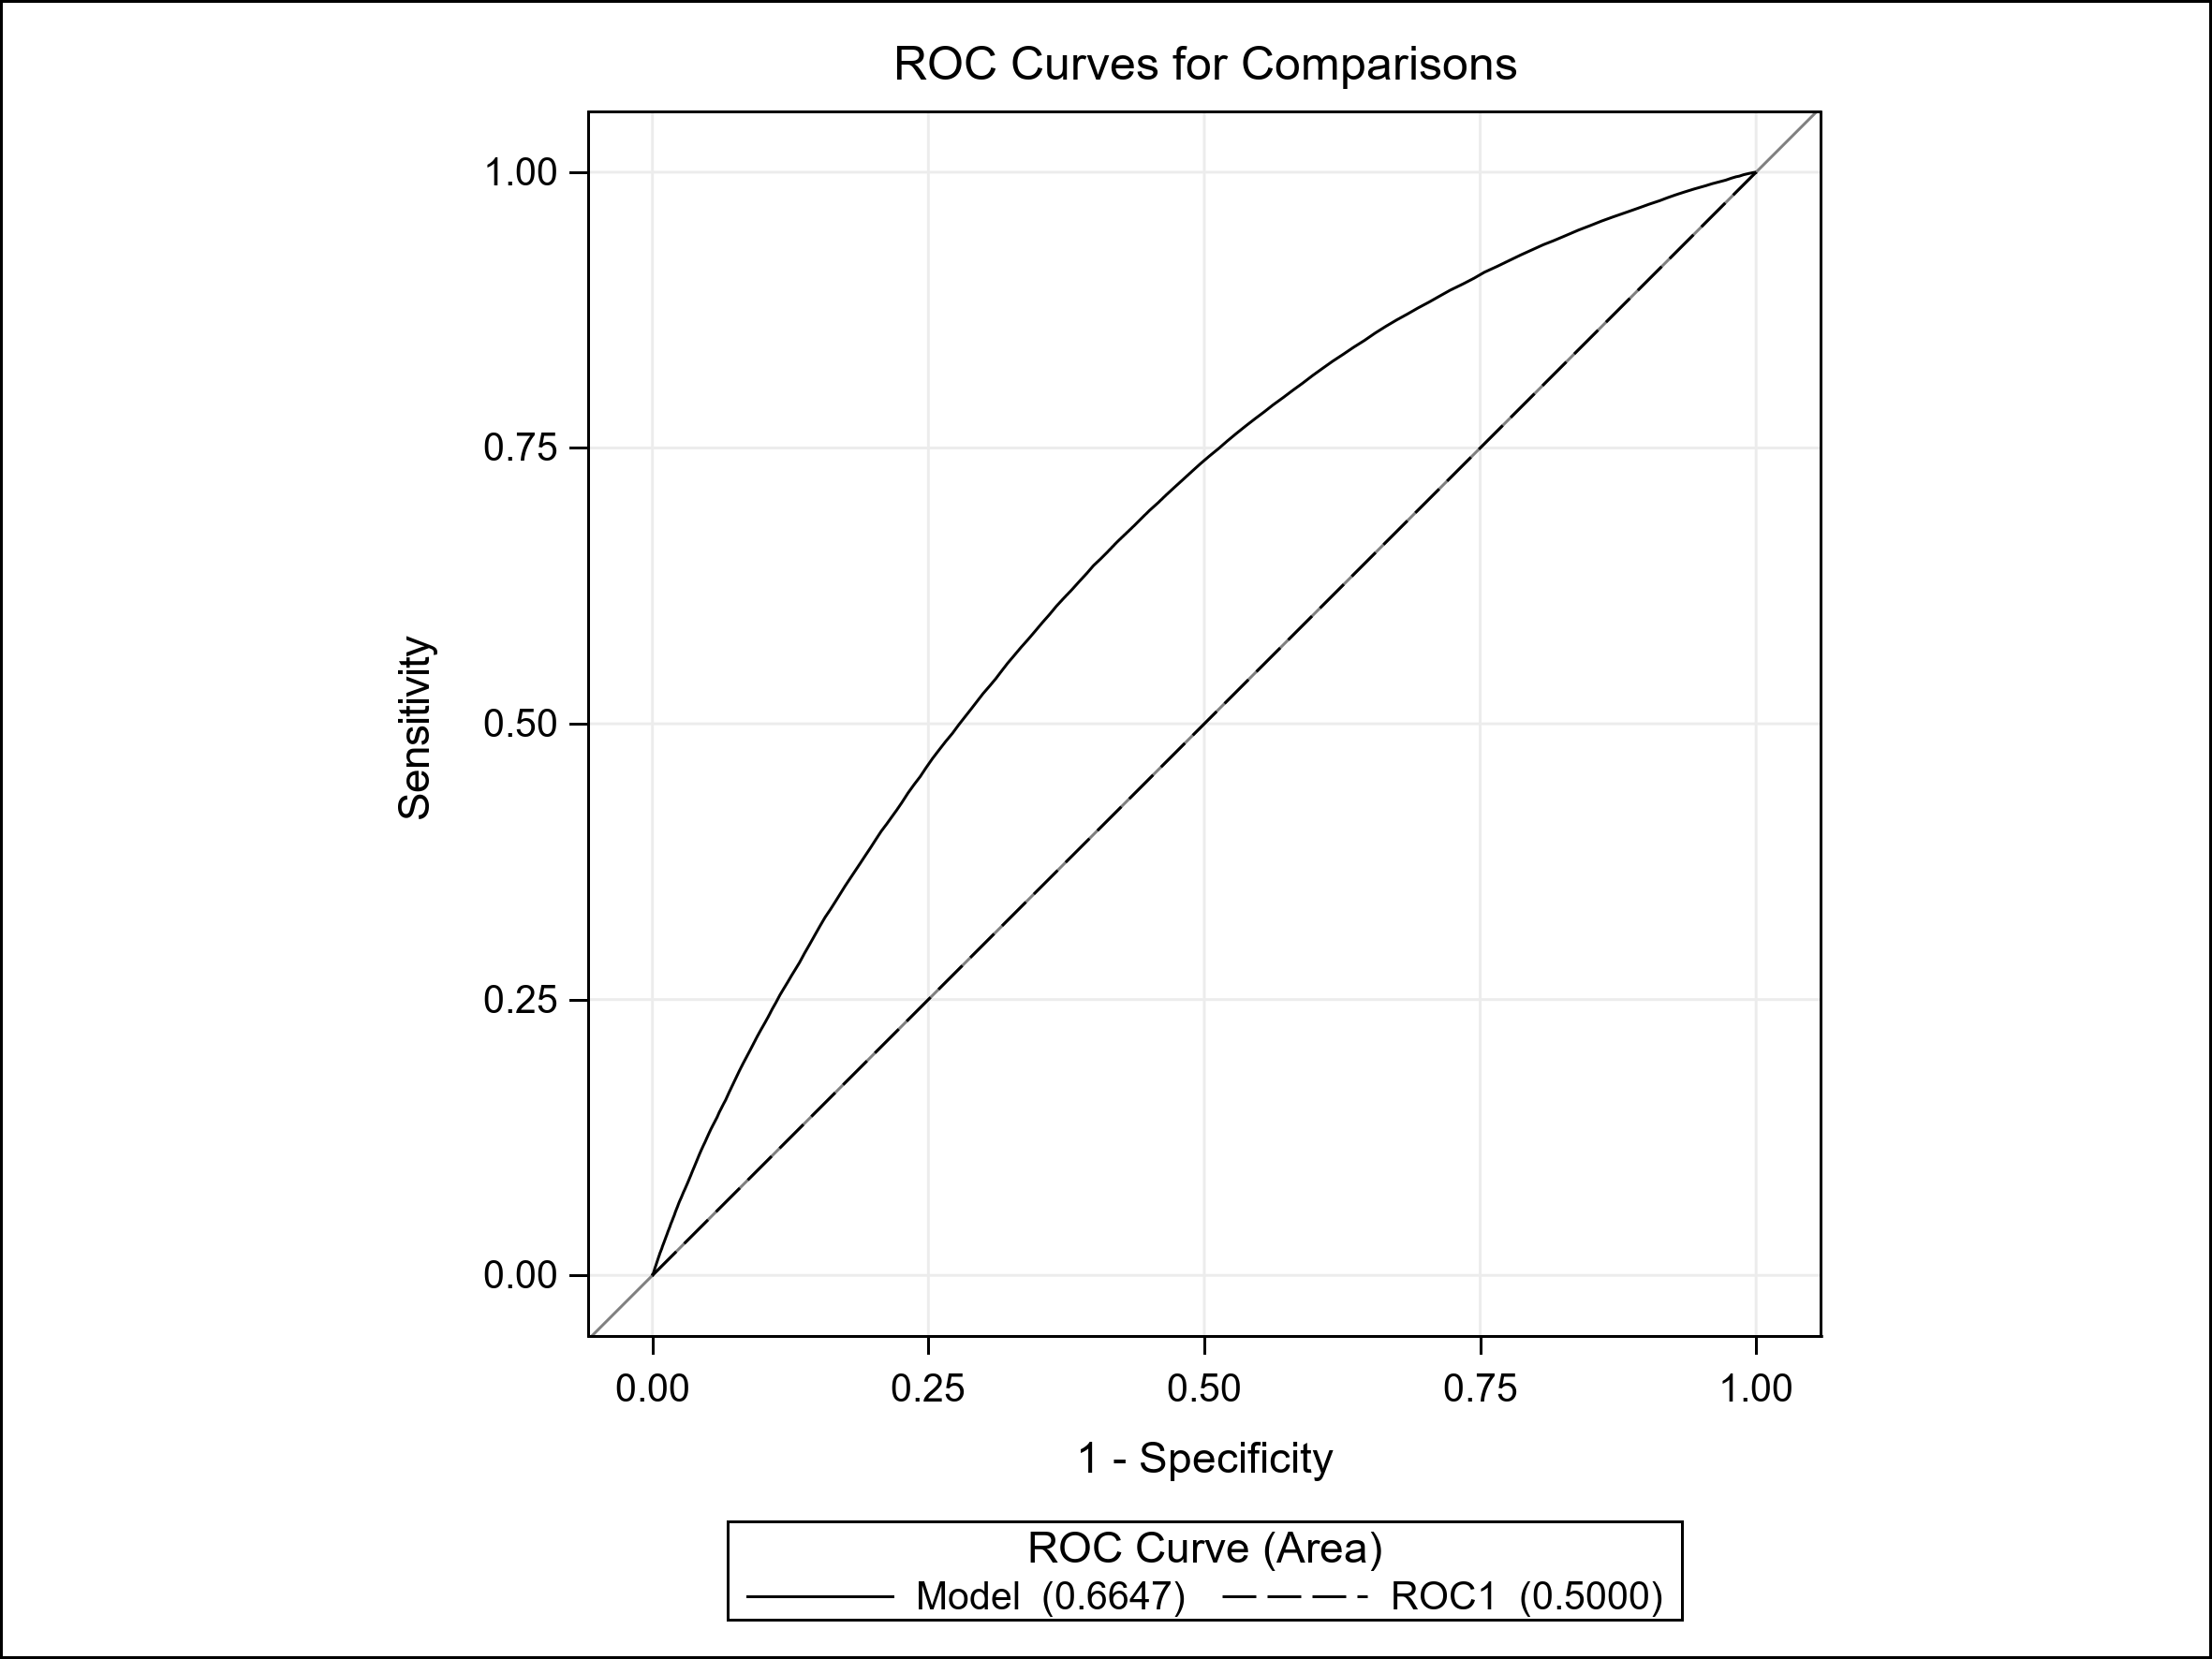
\includegraphics[width=0.9\textwidth]{./plot/ROC/Main/NUM_fico_ROC_ALL5.png}
\end{minipage}%
\begin{minipage}{.5\textwidth}
	\centering
	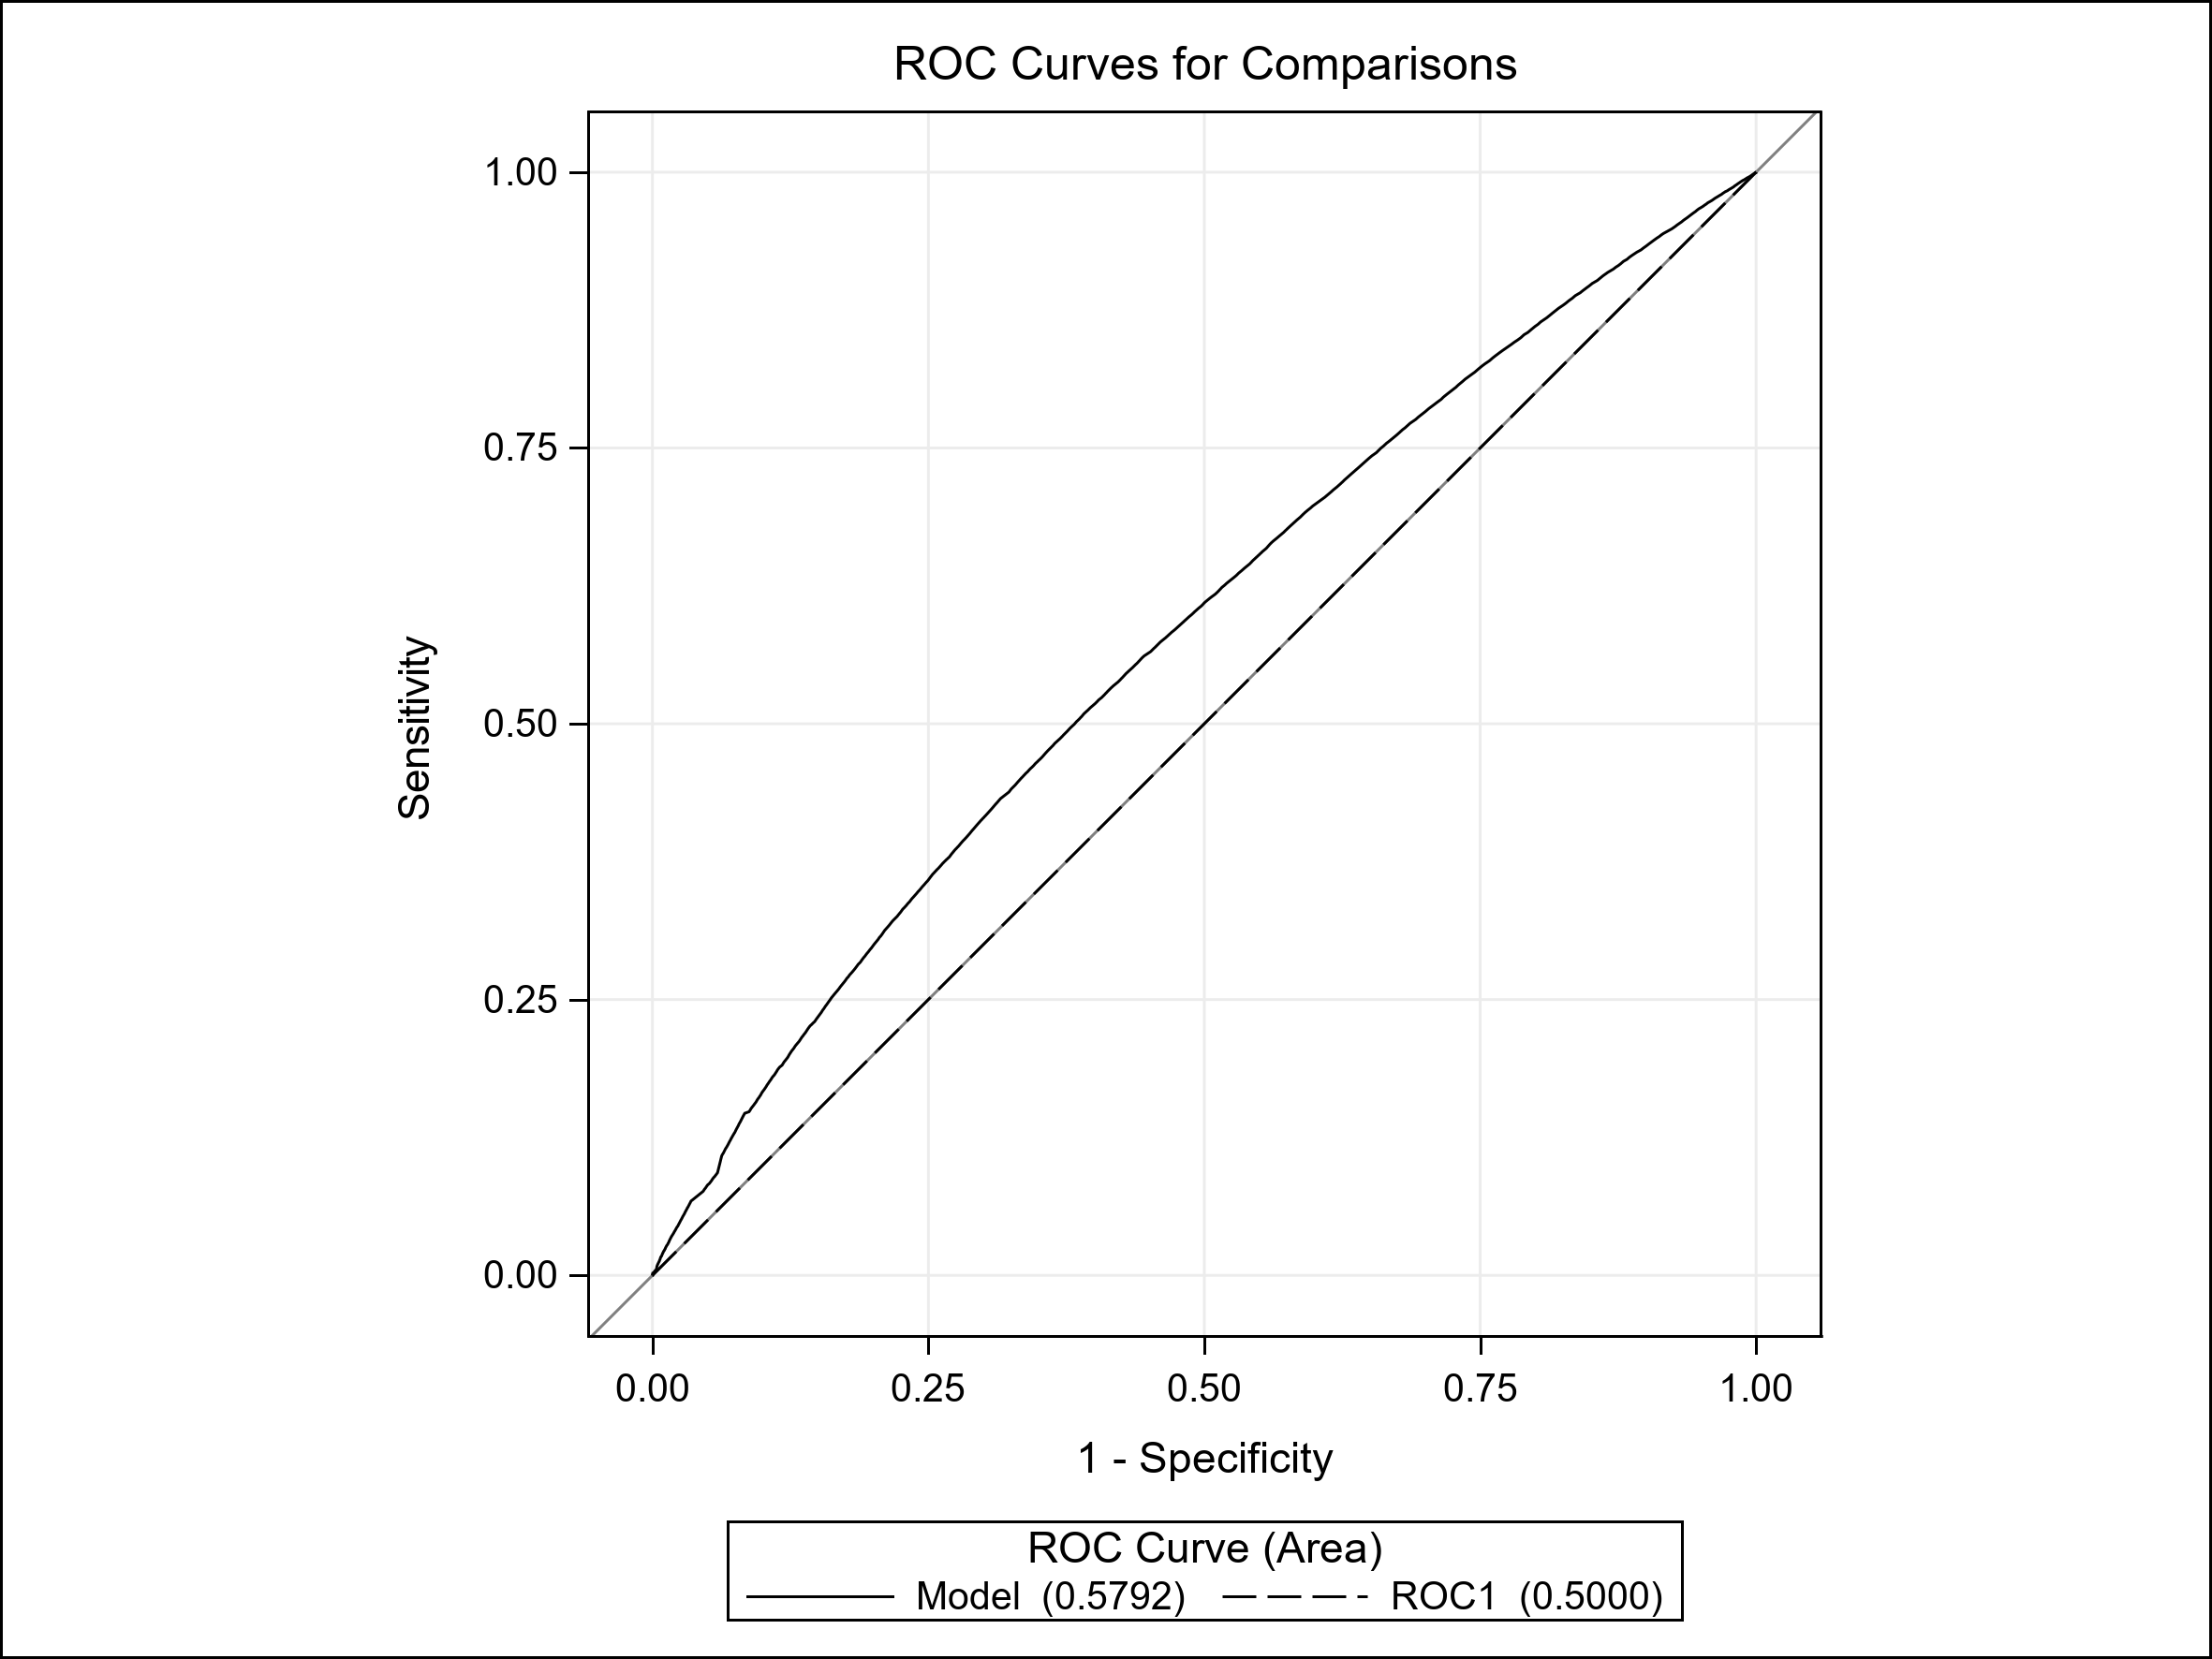
\includegraphics[width=0.9\textwidth]{./plot/ROC/Main/NUM_orig_upb_ROC_ALL5.png}
\end{minipage}
    \caption{ROC-curve of Credit Score (fico) and Original UPB}
    \label{fig:re_fico_upb}
\end{figure}
\begin{figure}[H]
\begin{minipage}{.5\textwidth}
	\centering
	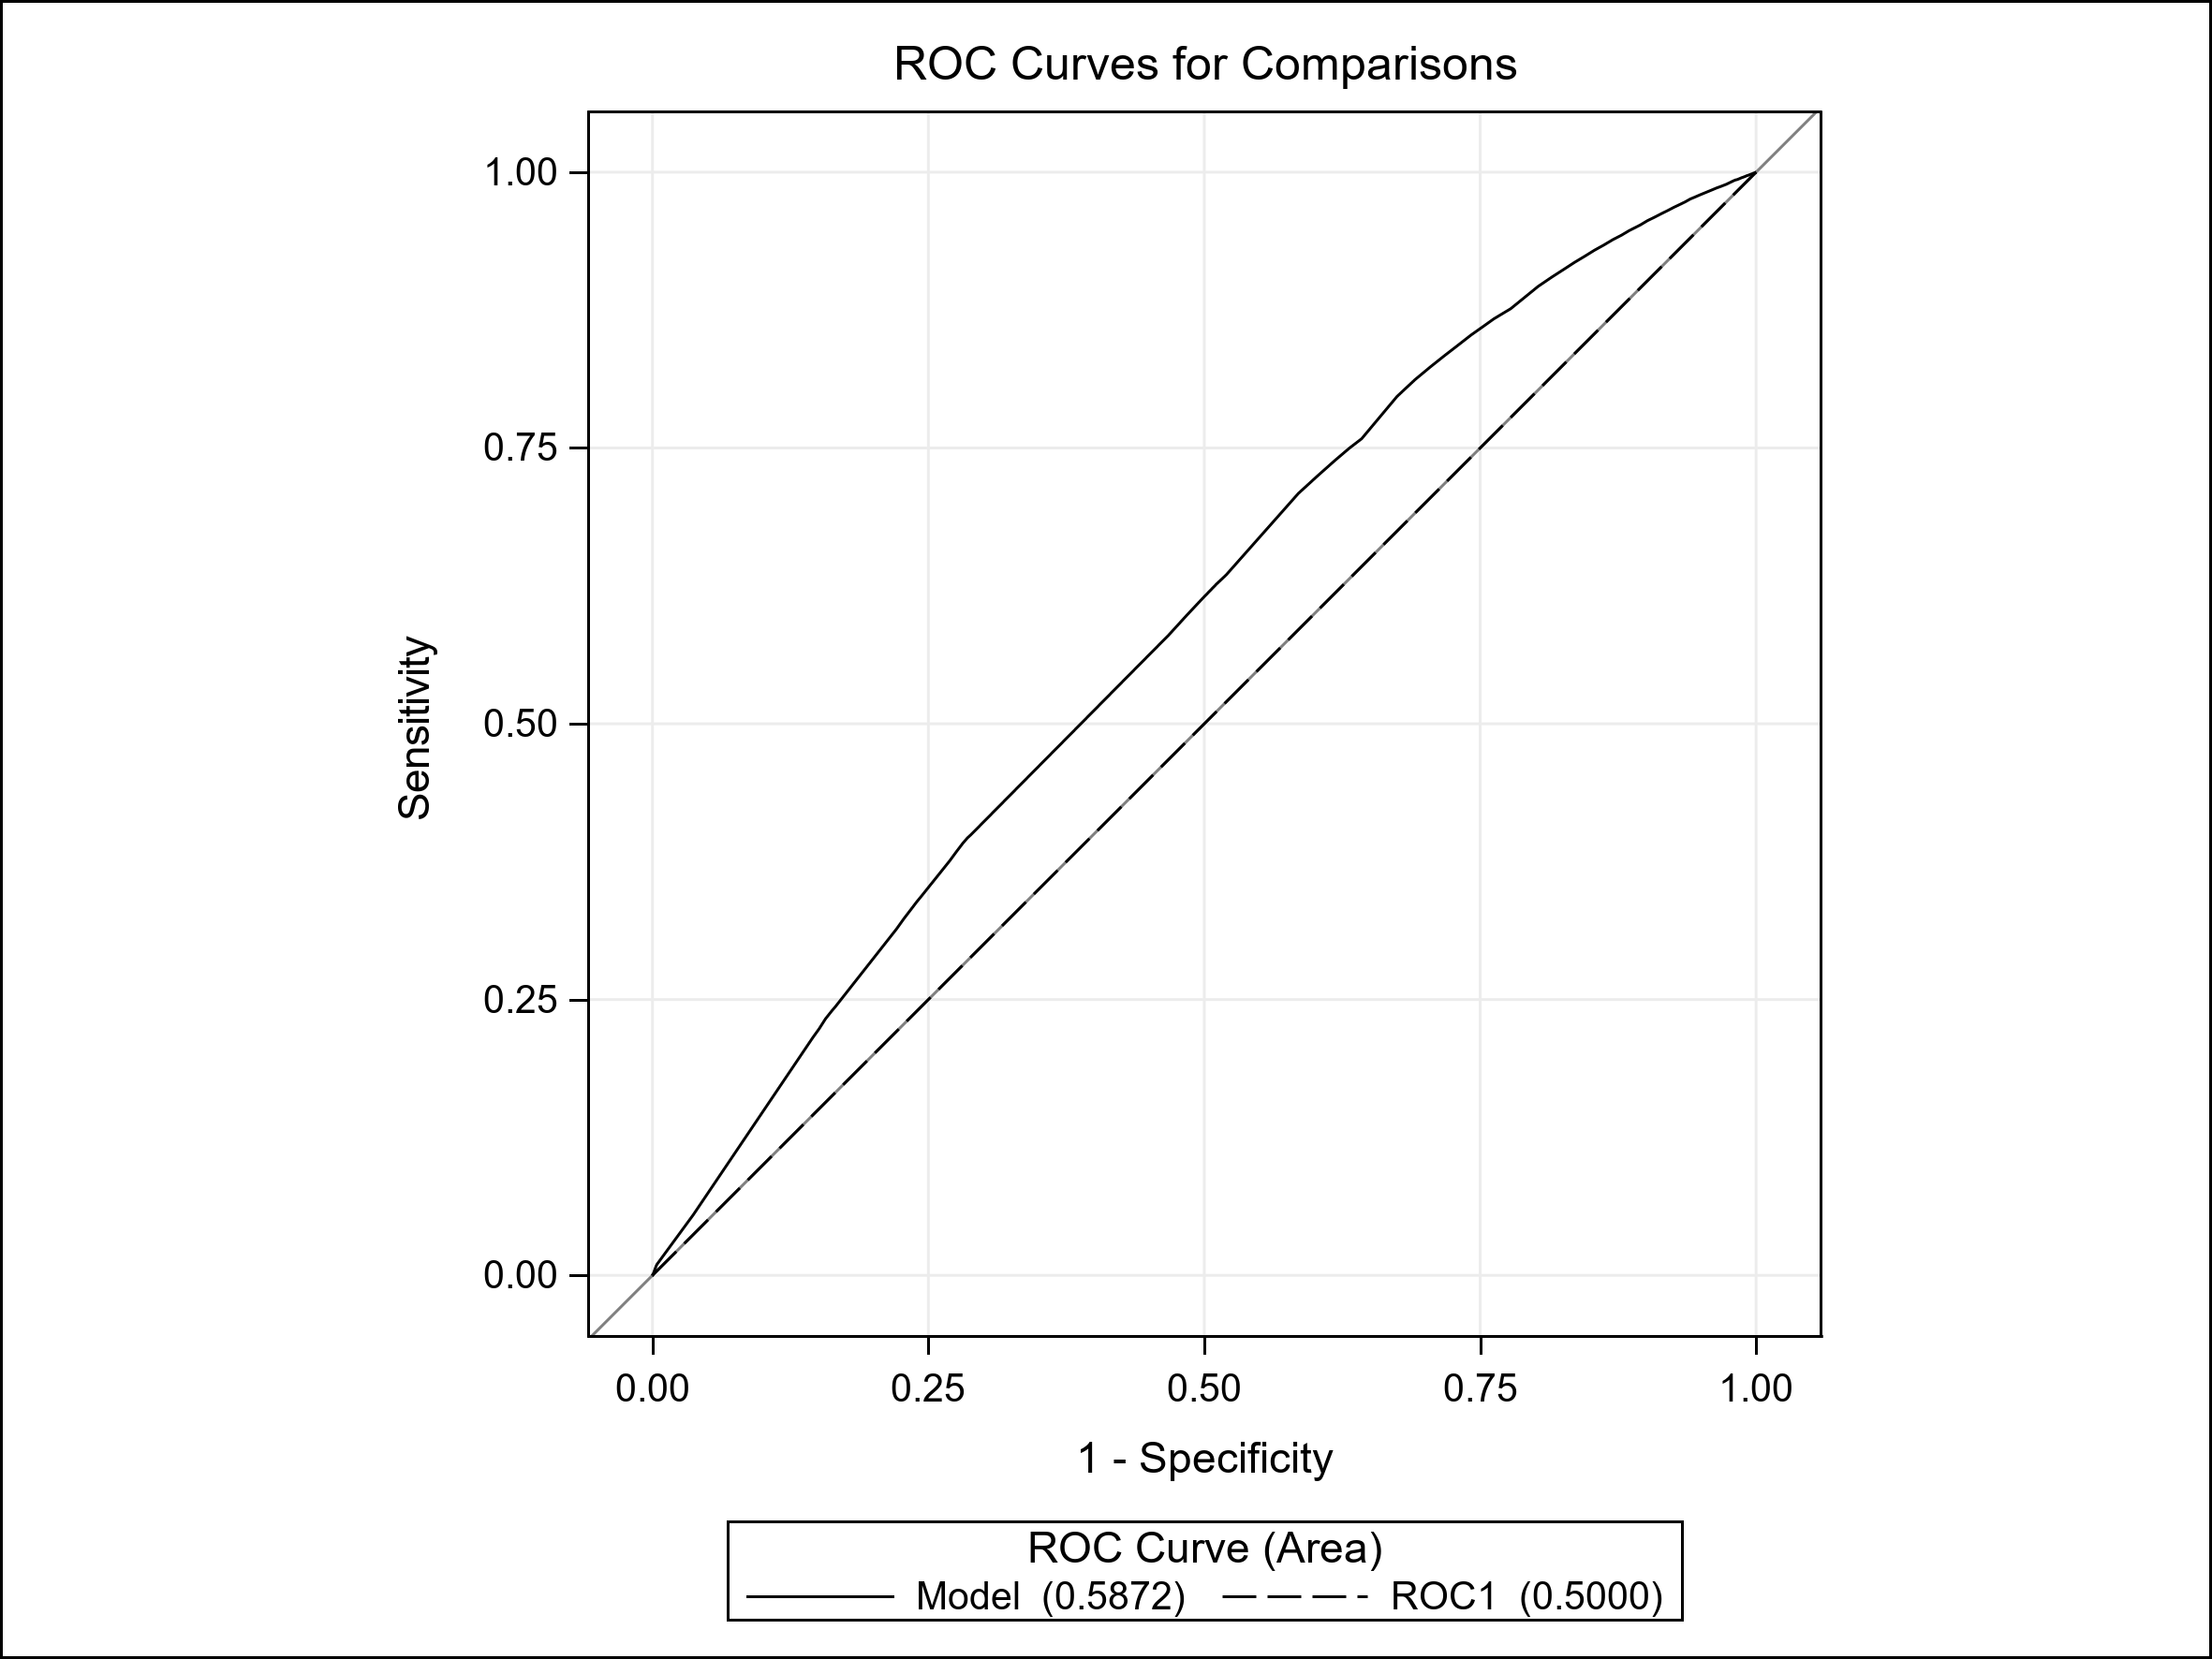
\includegraphics[width=0.9\textwidth]{./plot/ROC/Main/NUM_cltv_ROC_ALL5.png}
\end{minipage}%
\begin{minipage}{.5\textwidth}
	\centering
	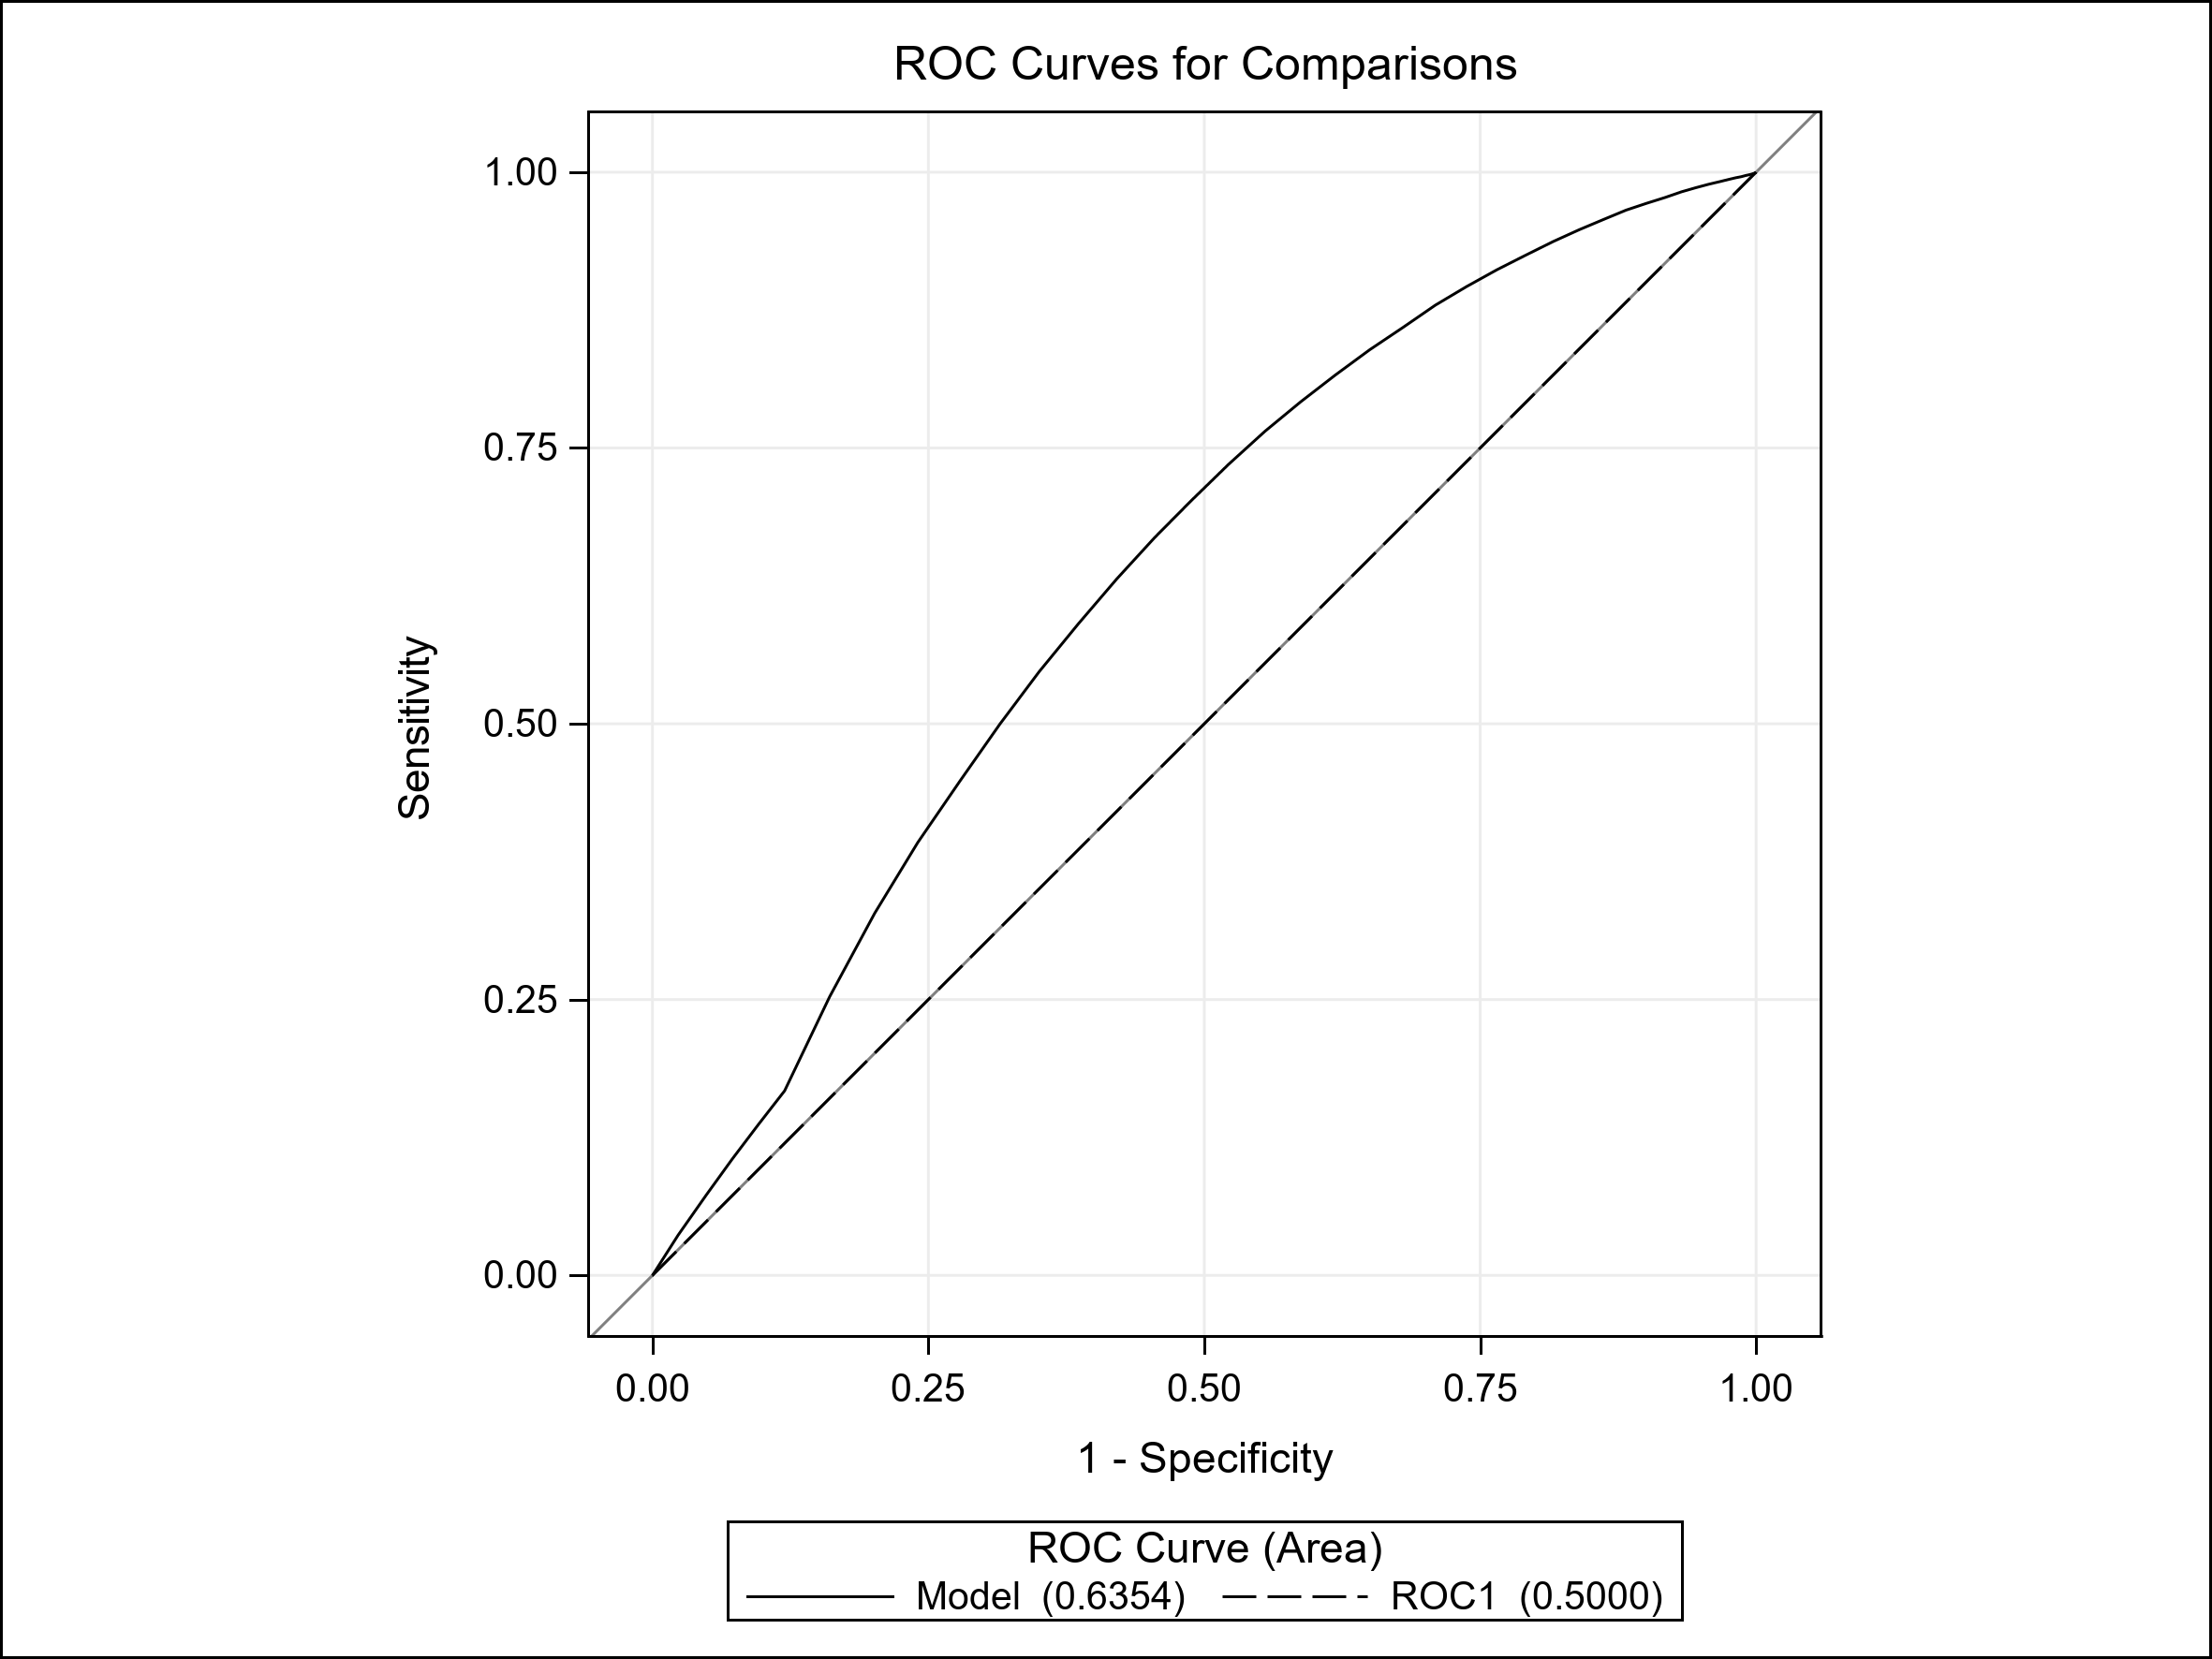
\includegraphics[width=0.9\textwidth]{./plot/ROC/Main/NUM_dti_ROC_ALL5.png}
\end{minipage}
    \caption{ROC-curve of CLTV and DTI}
    %\label{fig:dp_iqr_boxpl}
\end{figure}
\begin{figure}[H]
\begin{minipage}{.5\textwidth}
	\centering
	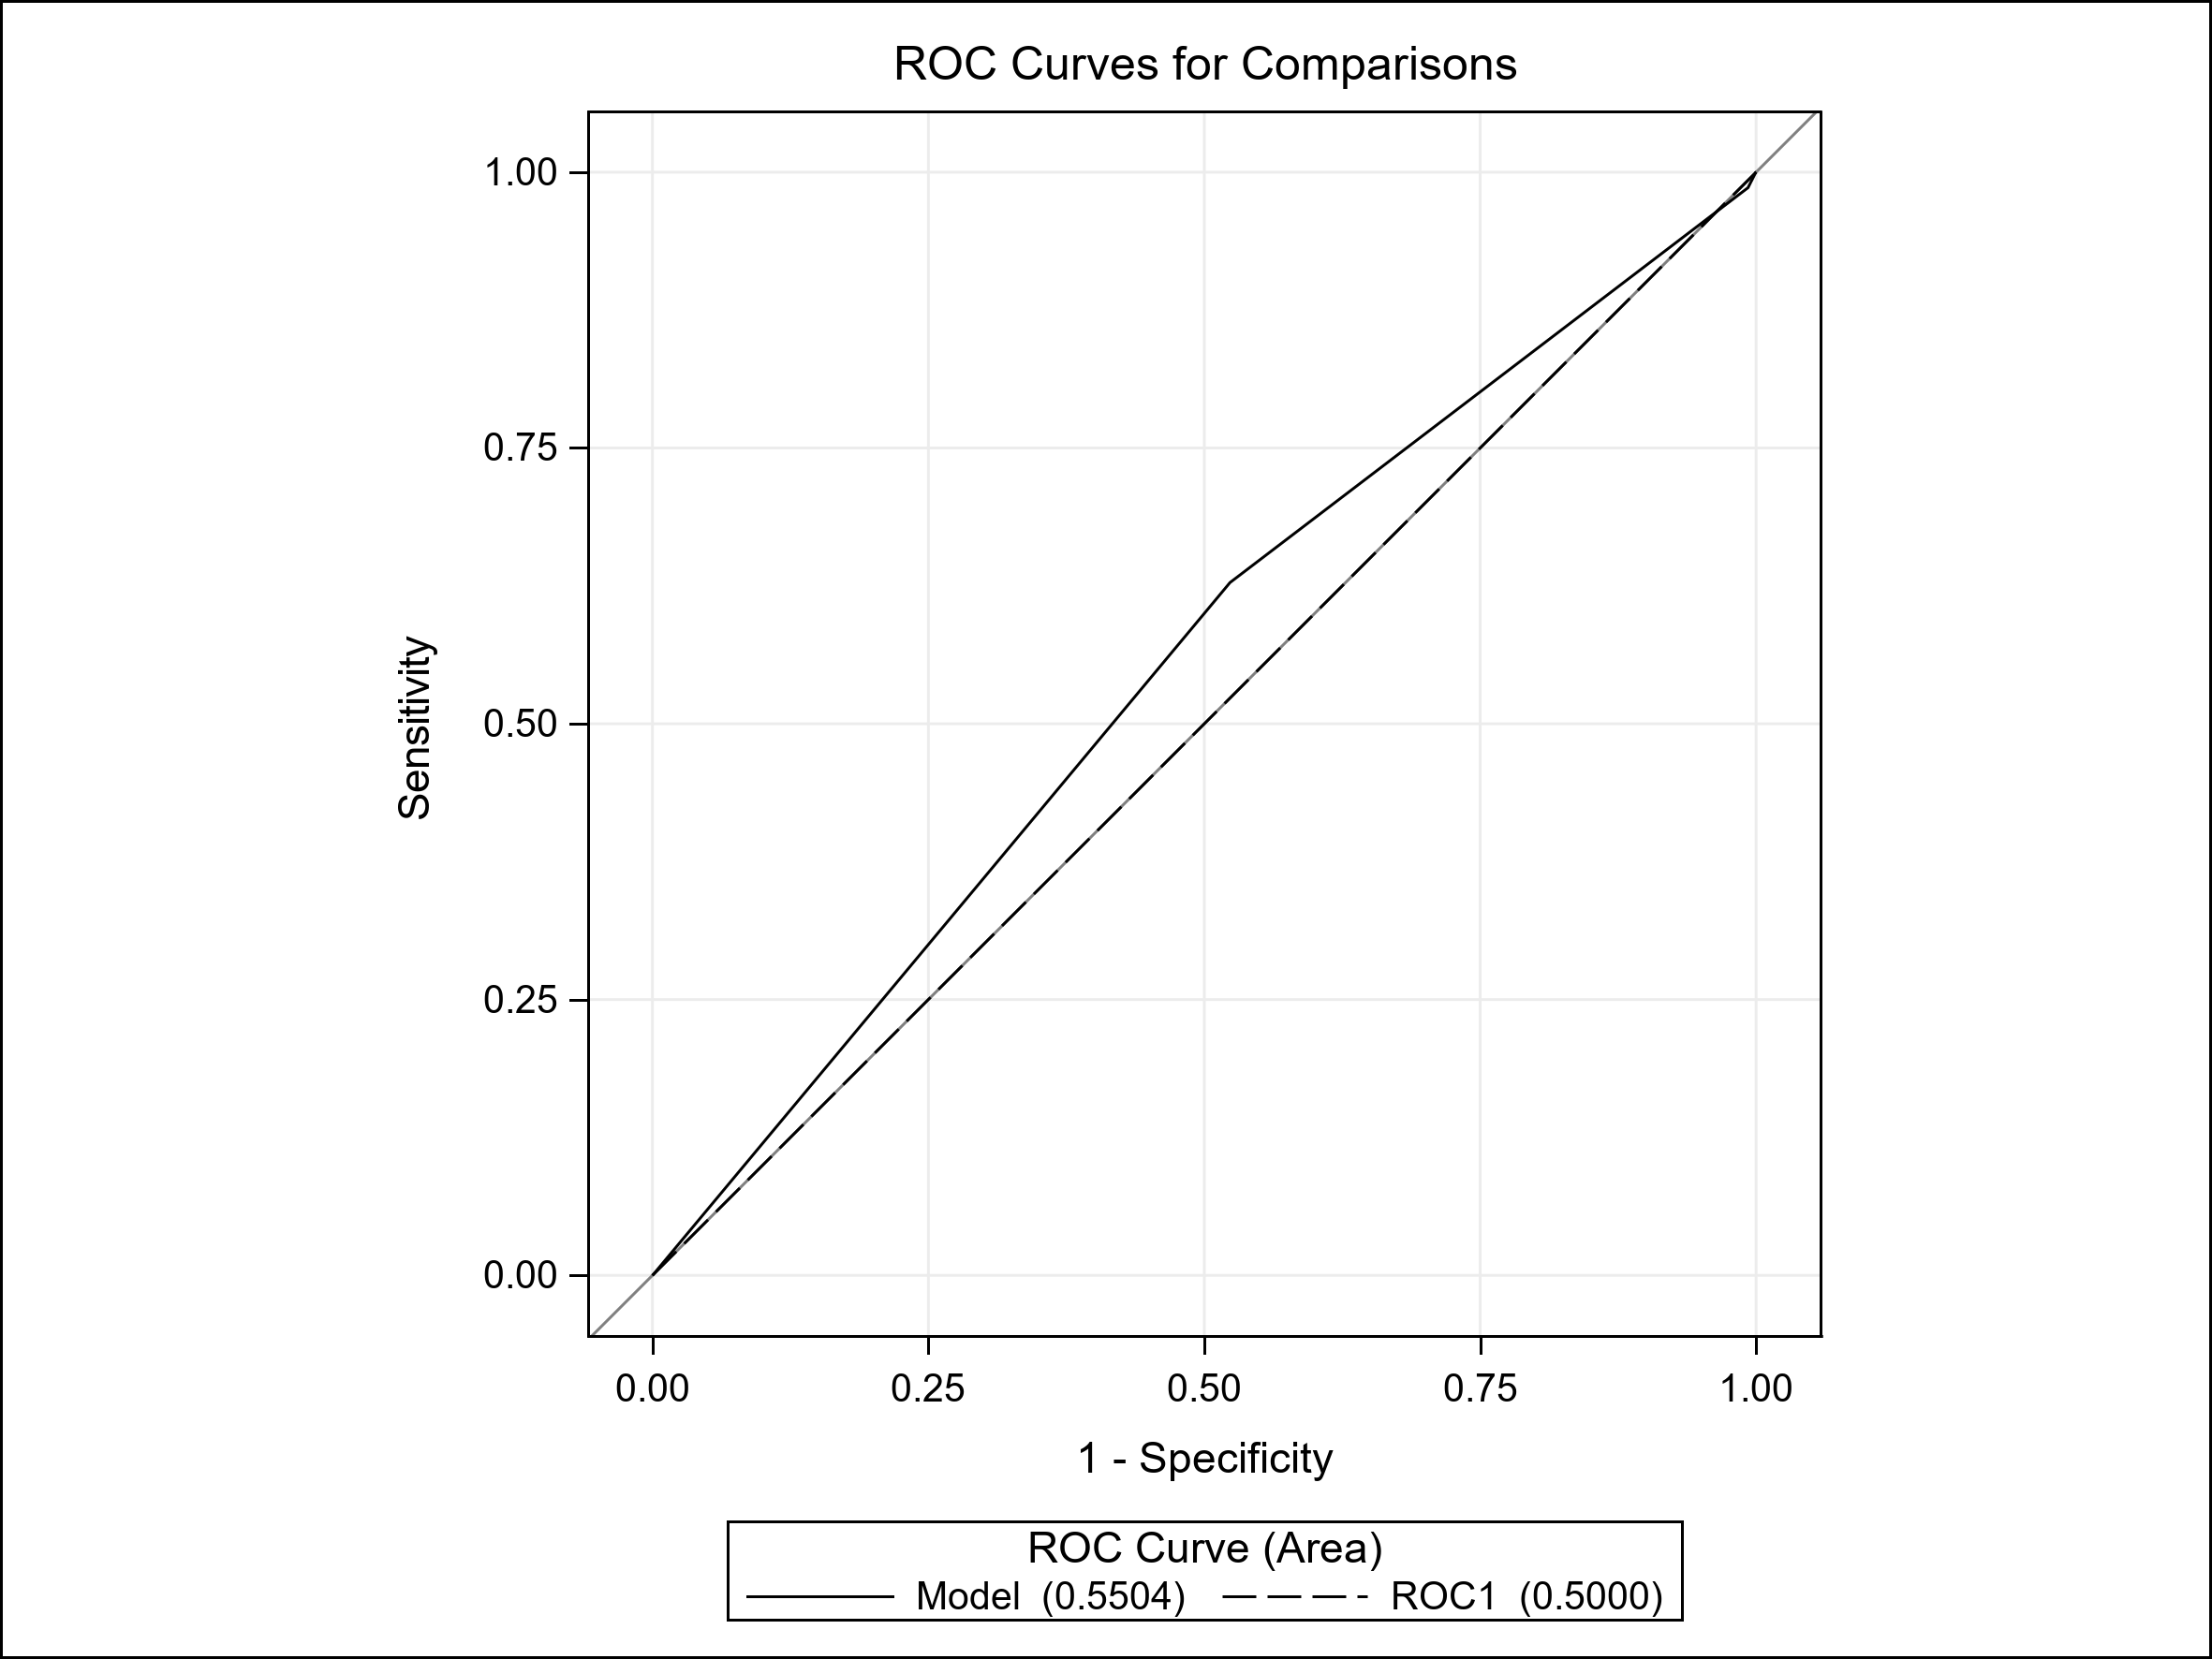
\includegraphics[width=0.9\textwidth]{./plot/ROC/Main/NUM_cnt_borr_ROC_ALL5.png}
\end{minipage}%
\begin{minipage}{.5\textwidth}
	\centering
	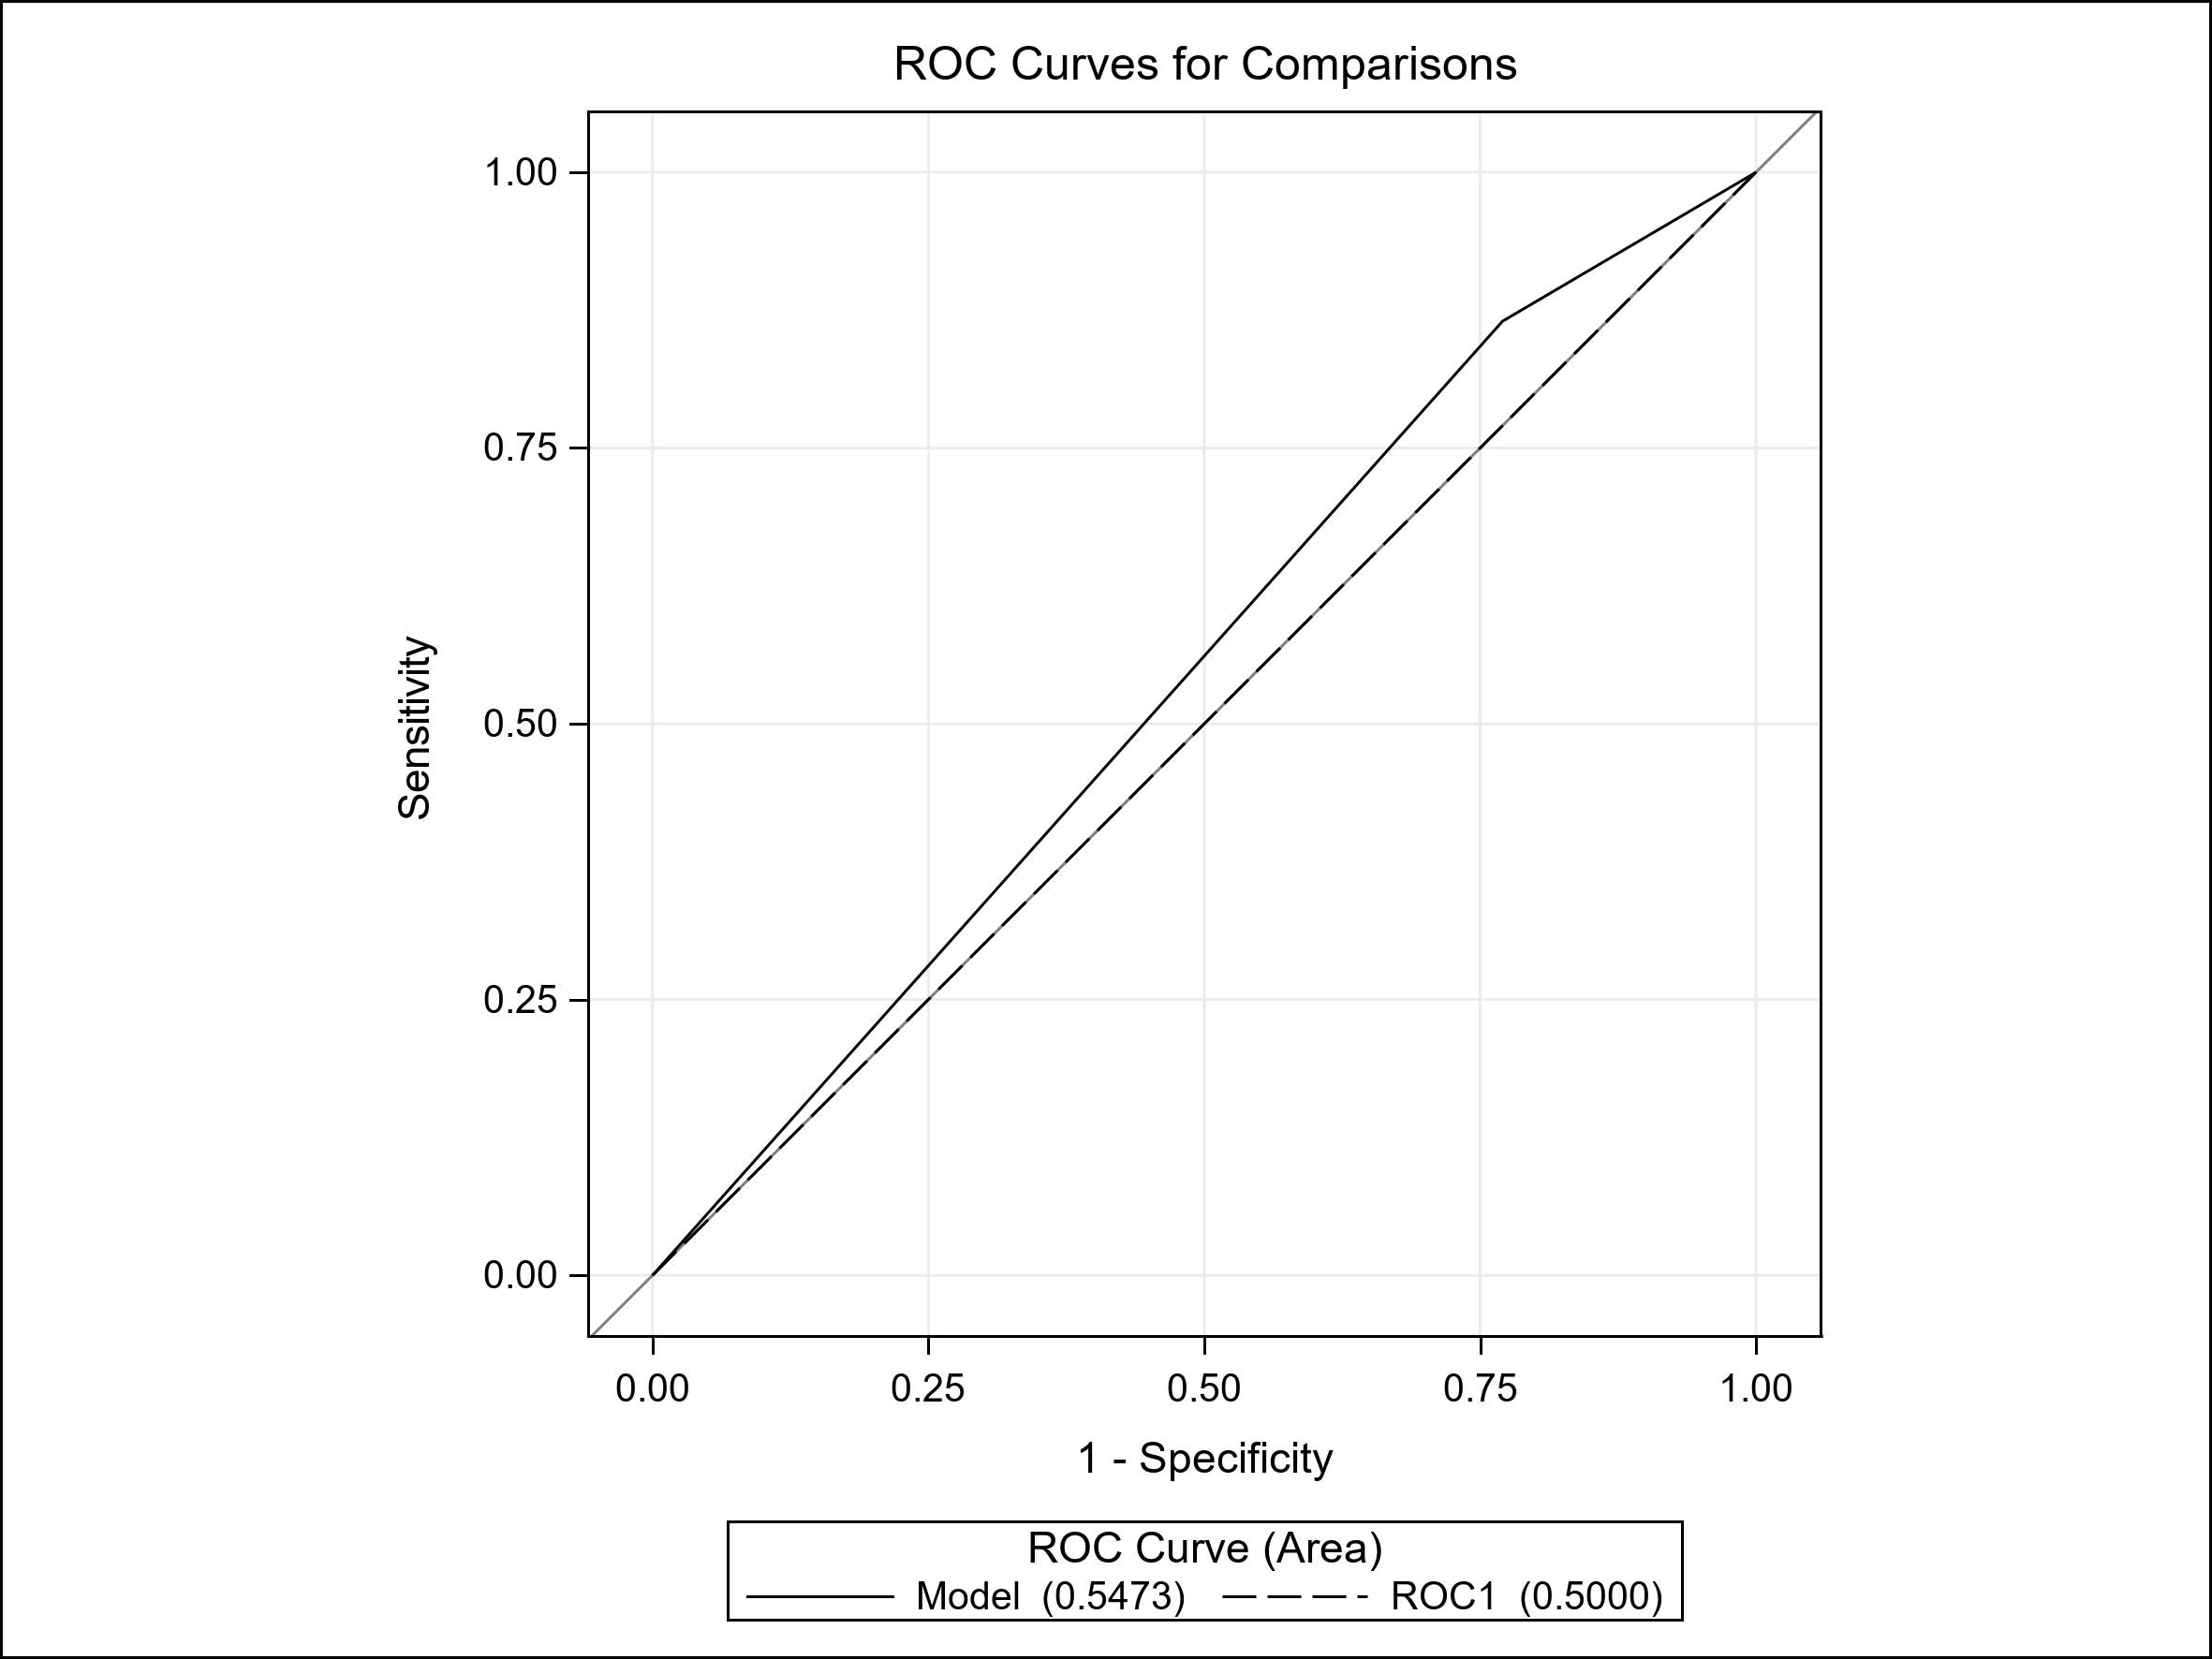
\includegraphics[width=0.9\textwidth]{./plot/ROC/Main/IND_flag_orig_loan_term_HEQ_360M_ROC_ALL5.png}
\end{minipage}
    \caption{ROC-curve of Number of Borrowers and Original Loan Term $\geq$ 360 months}
    %\label{fig:dp_iqr_boxpl}
\end{figure}
\begin{figure}[H]
\begin{minipage}{.5\textwidth}
	\centering
	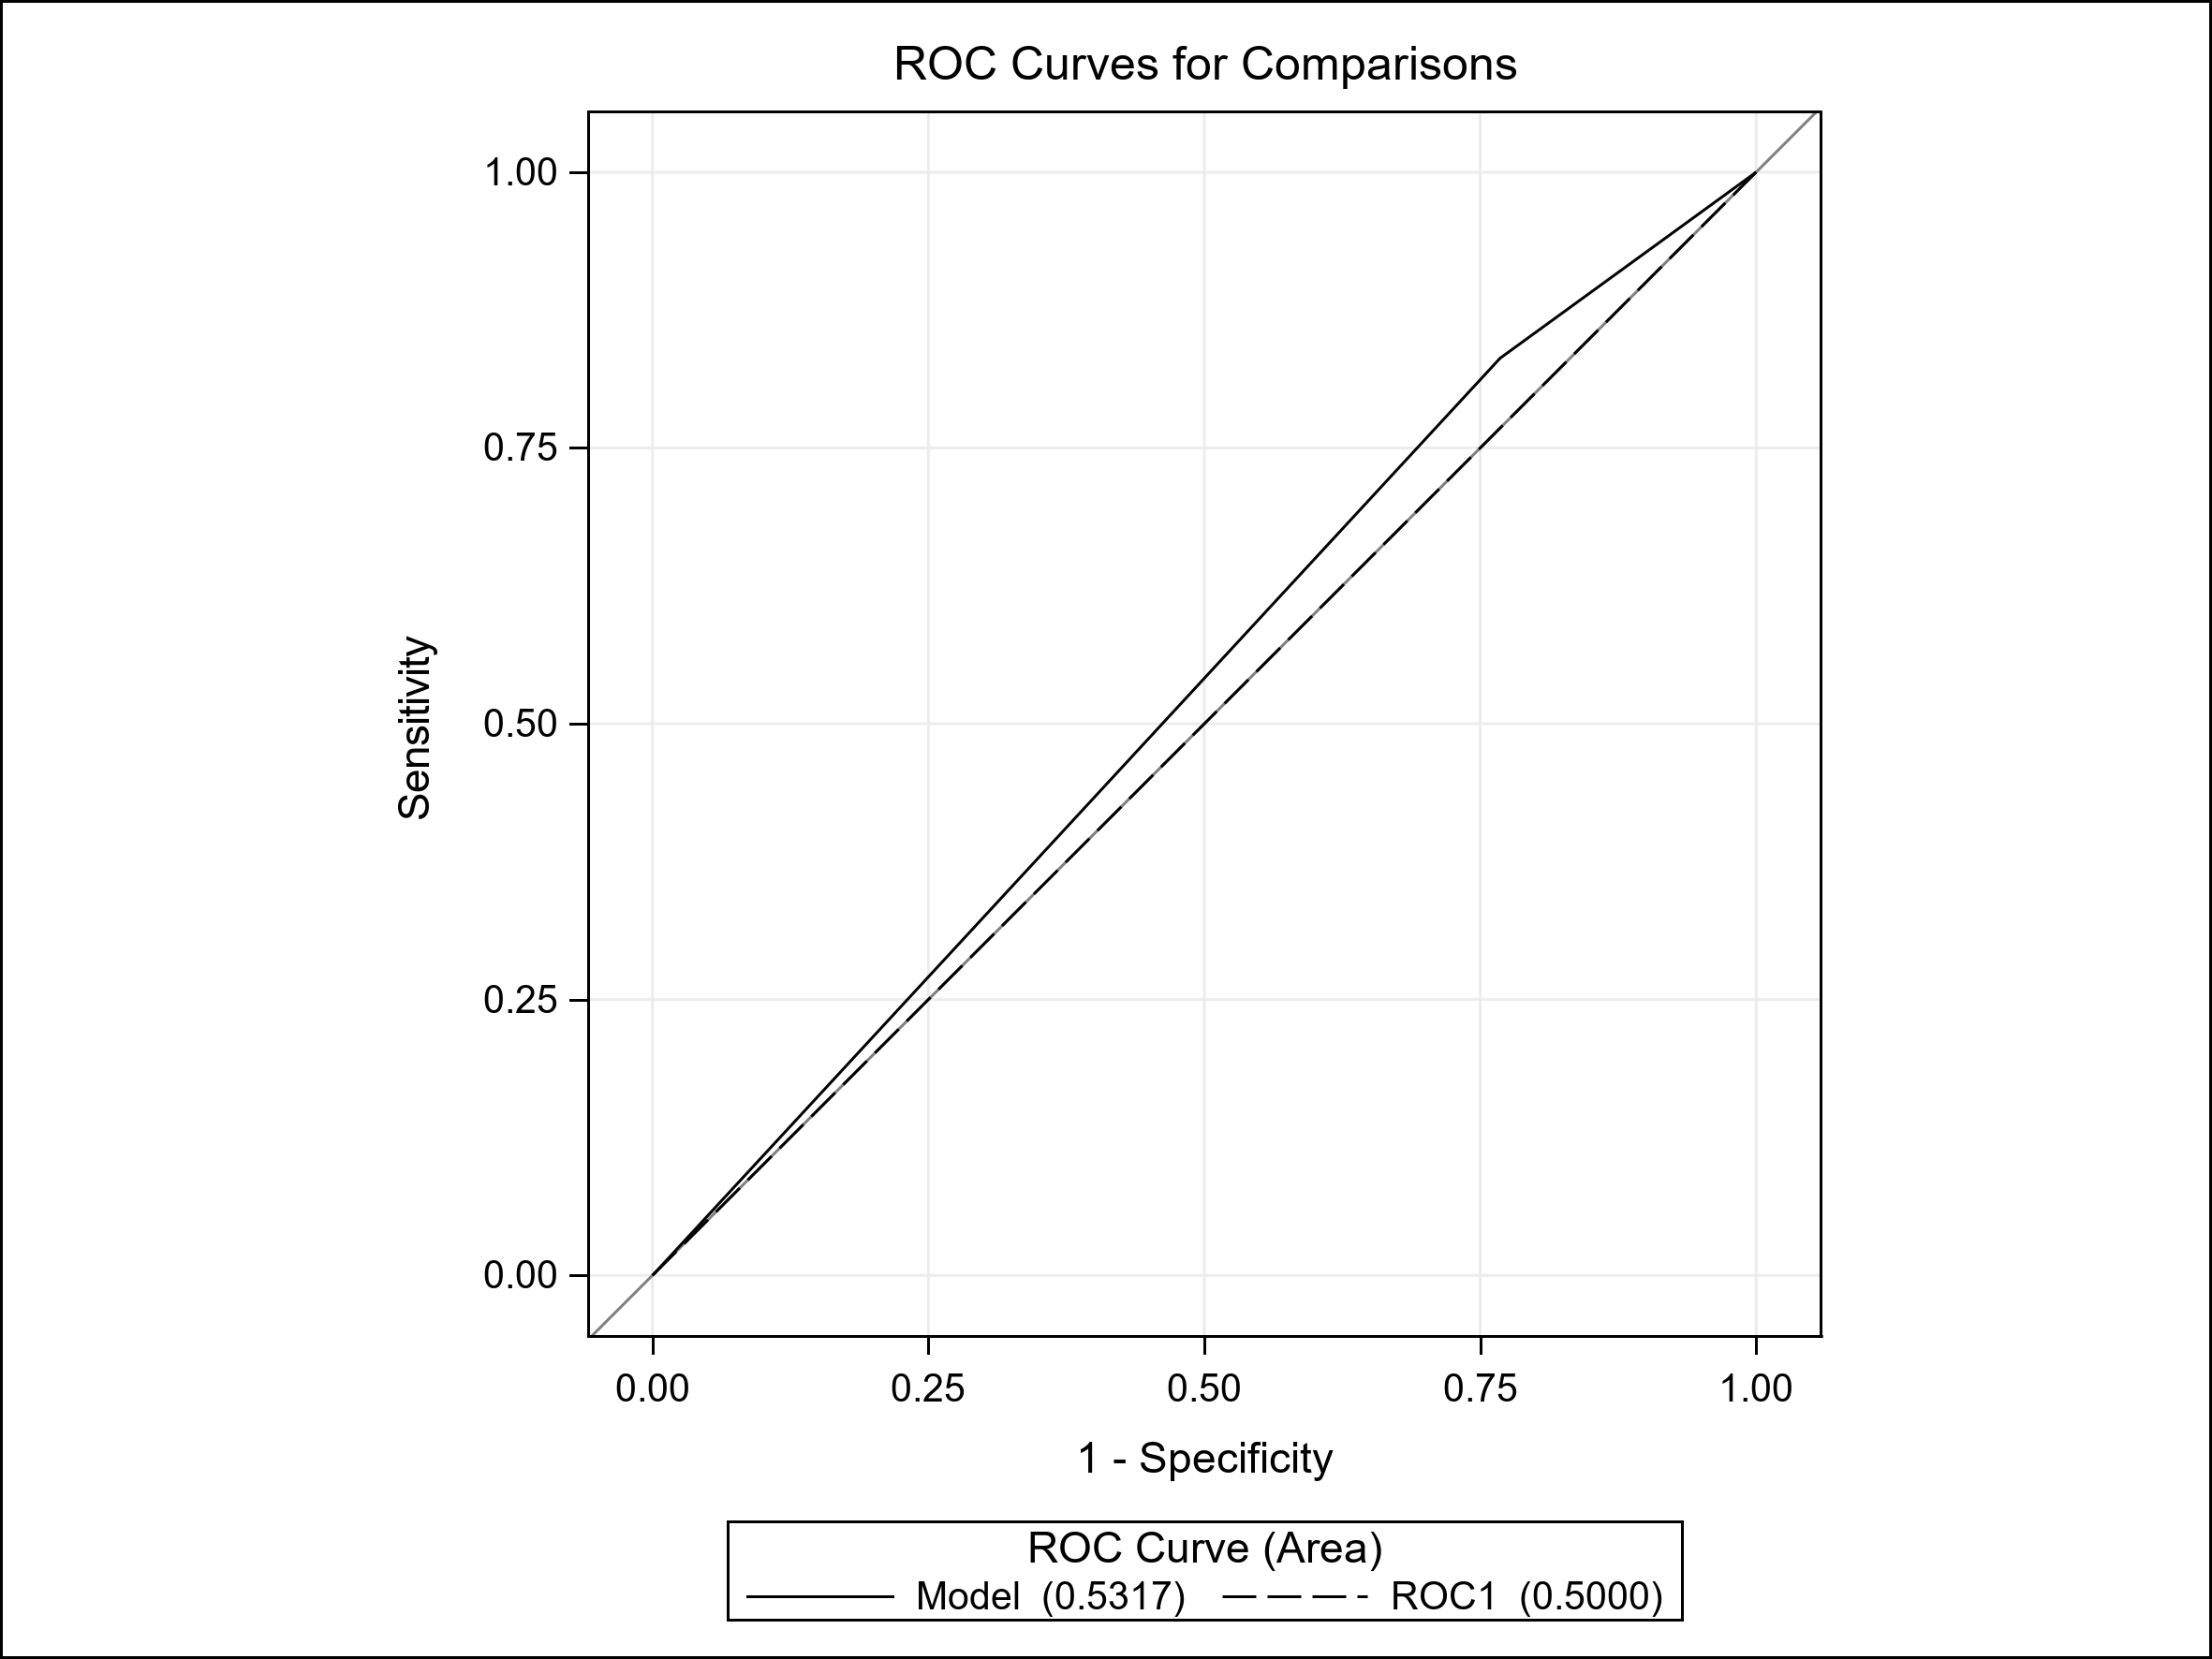
\includegraphics[width=0.9\textwidth]{./plot/ROC/Main/CAT_us_reg__Midwest_ROC_ALL5.png}
\end{minipage}%
\begin{minipage}{.5\textwidth}
	\centering
	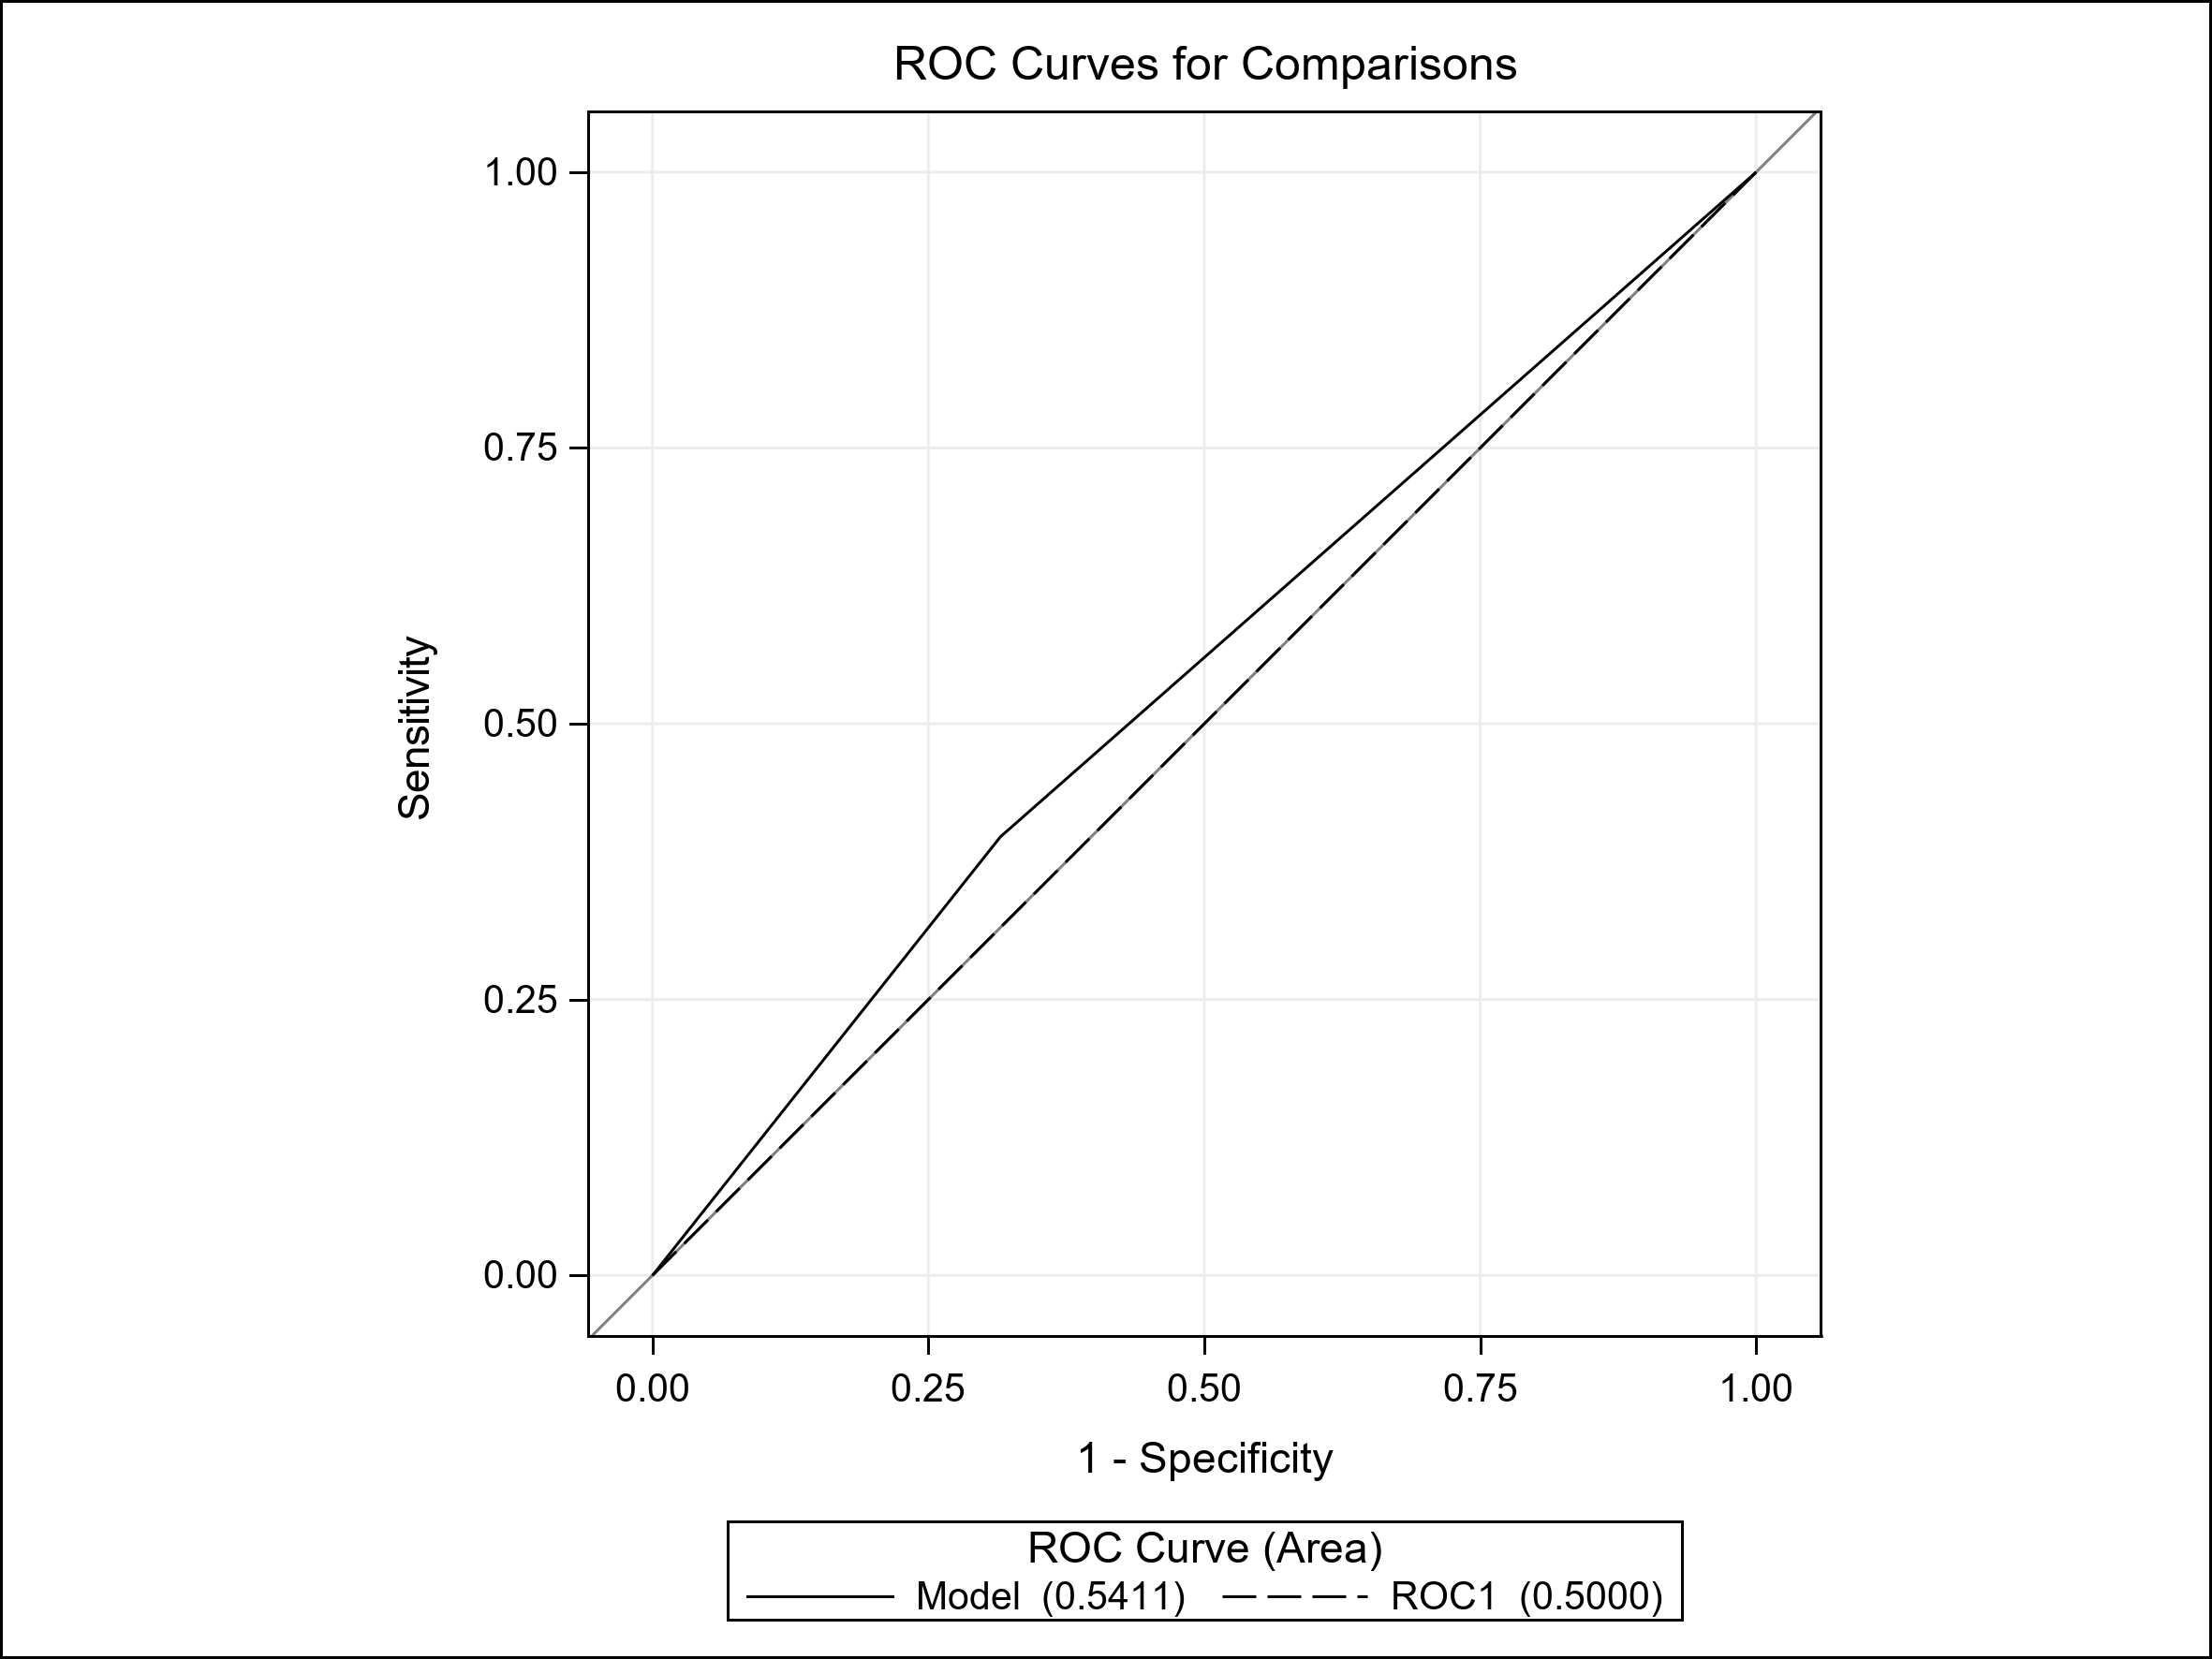
\includegraphics[width=0.9\textwidth]{./plot/ROC/Main/CAT_channel__C_ROC_ALL5.png}
\end{minipage}
    \caption{ROC-curve of US region = Midwest and Channel = Correspondent}
    \label{fig:re_usreg_channel}
\end{figure}

\subsection{Multivariate Analysis}

The shortlist was created using the following process: First, the correlation matrix with all numerical variables was created. Then, the variable with the highest GINI coefficient was identified and all risk factors with a correlation coefficient above +0.25 or below -0.25 were removed. This step should be repeated with the remaining variables until all features were analyzed. 
Table \ref{tab:re_corr_matrix} shows the correlation coefficient for all numeric variables in the long list. To account for potential interaction effects between categorical and indicator variables, the Variance Inflation Factor (VIF) was considered. A high correlation coefficient between \emph{LTV} and \emph{CLTV} is expected and a higher correlation is also visible between \emph{MI Perc}, \emph{Loan Term}, \emph{LTV} and \emph{CLTV}. Executing the described process, \emph{CLTV} was added to the shortlist, while the remaining correlated risk factors were excluded.  The VIF values, as shown in Table \ref{tab:re_vif}, do not indicate severe multicollinearity. In the final step, instead of using the raw variable, the indicator version \emph{Loan Term $\geq$ 360m} was chosen. The short list is given in Table \ref{tab:re_ll_sl}.

\begin{table}[H]
\resizebox{\textwidth}{!}{%
\begin{tabular}{ llllllllll }\toprule   
\textbf{Variable}     & \textbf{Credit Score} & \textbf{MI Perc}  & \textbf{No Units} & \textbf{CLTV}   & \textbf{DTI}   & \textbf{UPB} & \textbf{LTV} & \textbf{Loan Term} & \textbf{No Borrowers}\\\midrule
Credit Score & \cellcolor[HTML]{FFC7CE}{\color[HTML]{9C0006} 1,00} & -0,08                                               & 0,00                                                & -0,12                                               & -0,18                                               & 0,10                                                & -0,12                                               & -0,05                                               & -0,04                                               \\
MI Perc      & -0,08                                               & \cellcolor[HTML]{FFC7CE}{\color[HTML]{9C0006} 1,00} & -0,06                                               & \cellcolor[HTML]{FFC7CE}{\color[HTML]{9C0006} 0,67} & 0,10                                                & 0,03                                                & \cellcolor[HTML]{FFC7CE}{\color[HTML]{9C0006} 0,67} & \cellcolor[HTML]{FFC7CE}{\color[HTML]{9C0006} 0,26} & -0,05                                               \\
No Units     & 0,00                                                & -0,06                                               & \cellcolor[HTML]{FFC7CE}{\color[HTML]{9C0006} 1,00} & -0,05                                               & 0,04                                                & 0,06                                                & -0,05                                               & 0,02                                                & -0,02                                               \\
CLTV         & -0,12                                               & \cellcolor[HTML]{FFC7CE}{\color[HTML]{9C0006} 0,67} & -0,05                                               & \cellcolor[HTML]{FFC7CE}{\color[HTML]{9C0006} 1,00} & 0,13                                                & 0,09                                                & \cellcolor[HTML]{FFC7CE}{\color[HTML]{9C0006} 0,99} & \cellcolor[HTML]{FFC7CE}{\color[HTML]{9C0006} 0,33} & -0,06                                               \\
DTI          & -0,18                                               & 0,10                                                & 0,04                                                & 0,13                                                & \cellcolor[HTML]{FFC7CE}{\color[HTML]{9C0006} 1,00} & 0,06                                                & 0,13                                                & 0,13                                                & -0,08                                               \\
UPB          & 0,10                                                & 0,03                                                & 0,06                                                & 0,09                                                & 0,06                                                & \cellcolor[HTML]{FFC7CE}{\color[HTML]{9C0006} 1,00} & 0,09                                                & 0,16                                                & 0,15                                                \\
LTV          & -0,12                                               & \cellcolor[HTML]{FFC7CE}{\color[HTML]{9C0006} 0,67} & -0,05                                               & \cellcolor[HTML]{FFC7CE}{\color[HTML]{9C0006} 0,99} & 0,13                                                & 0,09                                                & \cellcolor[HTML]{FFC7CE}{\color[HTML]{9C0006} 1,00} & \cellcolor[HTML]{FFC7CE}{\color[HTML]{9C0006} 0,33} & -0,07                                               \\
Loan Term    & -0,05                                               & \cellcolor[HTML]{FFC7CE}{\color[HTML]{9C0006} 0,26} & 0,02                                                & \cellcolor[HTML]{FFC7CE}{\color[HTML]{9C0006} 0,33} & 0,13                                                & 0,16                                                & \cellcolor[HTML]{FFC7CE}{\color[HTML]{9C0006} 0,33} & \cellcolor[HTML]{FFC7CE}{\color[HTML]{9C0006} 1,00} & -0,06                                               \\
No Borrowers & -0,04                                               & -0,05                                               & -0,02                                               & -0,06                                               & -0,08                                               & 0,15                                                & -0,07                                               & -0,06                                               & \cellcolor[HTML]{FFC7CE}{\color[HTML]{9C0006} 1,00}           \\\bottomrule
\end{tabular}%
}
\caption{Correlation matrix}
\label{tab:re_corr_matrix}   
\end{table}

\begin{table}[H]
\centering
\begin{tabular}{p{8cm}cc}\toprule   
\textbf{Variable}                                                                & \textbf{VIF} 					& \textbf{p-value} \\\midrule
Credit Score                                                                     & 1,09                             & \textless{}.0001                     \\
DTI                                                                              & 1,09                             & \textless{}.0001                     \\
CLTV                                                                             & 2,08                             & \textless{}.0001                     \\
No Borrowers                                                                     & 1,02                             & \textless{}.0001                     \\
No Units                                                                         & 1,09                             & \textless{}.0001                     \\
Homebuyer Flag                                                                   & 1,57                             & \textless{}.0001                     \\
MI Flag                                                                          & 2,02                             & \textless{}.0001                     \\
Loan Term $\geq$ 360m                                                            & 1,22                             & \textless{}.0001                     \\
Channel = Not Available                                                          & 1,00                             & 0.7367                               \\
Channel = Broker                                                                 & 1,10                             & \textless{}.0001                     \\
Channel = Correspondent                                                          & 1,09                             & \textless{}.0001                     \\
Loan Purpose = Refinance - Cash Out    											 & 1,71                             & \textless{}.0001                     \\
Loan Purpose = Refinance - No Cash Out 											 & 2,08                             & \textless{}.0001                     \\
Prop Val Method = ACE Loans                                                      & 1,49                             & \textless{}.0001                     \\
Prop Val Method = Other Appraisals (Desktop, driveby, external, AVM)             & 1,03                             & \textless{}.0001                     \\
Prop Val Method = Not Available                                                  & 1,00                             & 0.6436                               \\
US Region = Midwest                                                              & 1,30                             & \textless{}.0001                     \\
US Region = Northeast                                                            & 1,23                             & \textless{}.0001                     \\
US Region = Other                                                                & 1,00                             & \textless{}.0001                     \\
US Region = West                                                                 & 1,40                             & \textless{}.0001                     \\
Occupancy = Second Home                                                          & 1,06                             & 0.0103                               \\
Occupancy = Investment Property                                                  & 1,16                             & \textless{}.0001                    \\\bottomrule
\end{tabular}
\caption{Variance Inflation Factor}
\label{tab:re_vif}   
\end{table}

\begin{longtable}{ l c c }\toprule    
\textbf{Variable}           & \textbf{Long List} 											& \textbf{Short List}						 \\\midrule
Credit Score                & \cellcolor[HTML]{C0F0C0}Missing Treatment applied            & \cellcolor[HTML]{C0F0C0}                     \\
Homebuyer Flag              & \cellcolor[HTML]{F7D9E1}Low GINI                             & -                                            \\
MI Perc                     & \cellcolor[HTML]{C0F0C0}Missing Treatment applied            & \cellcolor[HTML]{F7D9E1}Correlated with CLTV \\
No Units                    & \cellcolor[HTML]{F7D9E1}Low GINI                             & -                                            \\
Occupancy                   & \cellcolor[HTML]{F7D9E1}Low GINI                             & -                                            \\
CLTV                        & \cellcolor[HTML]{C0F0C0}Missing Treatment applied            & \cellcolor[HTML]{C0F0C0}                     \\
DTI                         & \cellcolor[HTML]{C0F0C0}Missing Treatment applied            & \cellcolor[HTML]{C0F0C0}                     \\
UPB                         & \cellcolor[HTML]{C0F0C0}                                     & \cellcolor[HTML]{C0F0C0}                     \\
LTV                         & \cellcolor[HTML]{C0F0C0}Missing Treatment applied            & \cellcolor[HTML]{F7D9E1}Correlated with CLTV \\
Channel                     & \cellcolor[HTML]{C0F0C0}                                     & \cellcolor[HTML]{C0F0C0}                     \\
PPM Flag                    & \cellcolor[HTML]{F7D9E1}Low GINI                             & -                                            \\
Amort Type                  & \cellcolor[HTML]{F7D9E1}Low GINI                             & -                                            \\
State                       & \cellcolor[HTML]{F7D9E1}Adapted Variable derived (US-region) & -                                            \\
Prop Type                   & \cellcolor[HTML]{F7D9E1}Low GINI                             & -                                            \\
Loan Purpose                & \cellcolor[HTML]{F7D9E1}Low GINI                             & -                                            \\
Loan Term                   & \cellcolor[HTML]{C0F0C0}                                     & \cellcolor[HTML]{F7D9E1}Correlated with CLTV \\
No Borrowers                & \cellcolor[HTML]{C0F0C0}                                     & \cellcolor[HTML]{C0F0C0}                     \\
Sup Conf Flag               & \cellcolor[HTML]{F7D9E1}High Missing Rate                    & -                                            \\
Prog Flag                   & \cellcolor[HTML]{F7D9E1}High Missing Rate                    & -                                            \\
HARP Flag                   & \cellcolor[HTML]{F7D9E1}High Missing Rate                    & -                                            \\
Prop Val Method             & \cellcolor[HTML]{C0F0C0}                                     & \cellcolor[HTML]{C0F0C0}                     \\
Int Only Flag               & \cellcolor[HTML]{F7D9E1}Low GINI                             & -                                            \\
US Region                   & \cellcolor[HTML]{C0F0C0}                                     & \cellcolor[HTML]{C0F0C0}                     \\
MI Flag                     & \cellcolor[HTML]{C0F0C0}                                     & \cellcolor[HTML]{C0F0C0}                     \\
Loan Term \textgreater 360m & \cellcolor[HTML]{F7D9E1}Low GINI                             & -                                            \\
Loan Term Group             & \cellcolor[HTML]{F7D9E1}Similar Variable used                & -                                            \\
Loan Term $\geq$ 360m       & \cellcolor[HTML]{C0F0C0}                                     & \cellcolor[HTML]{C0F0C0}                     \\
Loan Term = 360m            & \cellcolor[HTML]{F7D9E1}Similar Variable used                & -                                           \\\bottomrule
\caption{Long list and Short list}
\label{tab:re_ll_sl}       
\end{longtable}

\subsection{Scaling}
Due to the different ranges of risk factors, especially because of \emph{Original Unpaid Balance}, a standardization of all numeric variables was carried out to prevent unusually small or large coefficients. The following formula is used:

\begin{equation}
X_{\text{standardized}} = \frac{X - \mu}{\sigma}
\end{equation}
where:
\begin{conditions}
 X  	& original variable \\
\mu		& mean of the variable \\
\sigma	& standard deviation of the variable
\end{conditions}

\section{Modeling}

\subsection{Logistic Regression}
Employing the stepwise selection algorithm, all short list variables were inserted into the modeling process, resulting in the model presented in Table \ref{tab:re_prelLogModel}. The order of the risk factors indicates the significance in the model, with all coefficients exhibiting statistical significance indicated by low p-values. The AIC and BIC were calculated at each modeling step to limit the number of explanatory variables. Table \ref{tab:re_AICBIC} outlines the relative change per step. A noticeable drop in improvement occurs between step 5 and 6 and thus, prompting the removal of all succeeding variables, followed by a re-estimation of the model. The final model, detailed in Table \ref{tab:re_finalLogModel}, only includes numeric variables. All coefficients align with the expected economic sign; for example, a higher DTI corresponds to a higher probability of default, reflected in a positive coefficient. In contrast, an increased number of borrowers, which means more people are obligated to repay the loan, correlates with a lower probability of default, resulting in a negative coefficient. Performance metrics for the model are provided in Chapter \ref{sec:comp_model} as part of the comparison with the Random Forest model.

\begin{table}[H]
\centering
\begin{tabular}{p{8cm}rr}\toprule
\textbf{Parameter}                                                   & \textbf{Coefficient} & \textbf{p-value} \\\midrule
Intercept                                                            & -4,892               & \textless{}.0001 \\
Credit Score                                                         & -0,542               & \textless{}.0001 \\
DTI                                                         		 & 0,392                & \textless{}.0001 \\
CLTV                                                                 & 0,223                & \textless{}.0001 \\
UPB                                                                  & 0,316                & \textless{}.0001 \\
No Borrowers                                                         & -0,245               & \textless{}.0001 \\
Loan Term $\geq$ 360m                                                & 0,144                & \textless{}.0001 \\
Channel = Broker                                                     & 0,104                & \textless{}.0001 \\
Channel = Correspondent                                              & 0,279                & \textless{}.0001 \\
Prop Val Method = Other Appraisals (Desktop, driveby, external, AVM) & -0,206               & \textless{}.0001 \\
Prop Val Method = Full Appraisal                                     & 0,180                & \textless{}.0001 \\
US Region = Midwest                                                  & -0,152               & \textless{}.0001 \\
US Region = Northeast                                                & 0,138                & \textless{}.0001 \\
US Region = Other                                                    & 0,869                & \textless{}.0001\\\bottomrule
\end{tabular}
\caption{Preliminary Logit Model}
\label{tab:re_prelLogModel}
\end{table}

\begin{table}[H]
\centering
\begin{tabular}{lccccp{4cm}}\toprule
\textbf{Step} & \textbf{AIC} & \textbf{rel. AIC ch.} & \textbf{BIC} & \textbf{rel. BIC ch.} & \textbf{Variable added}                                              \\\midrule
1             & 577821       &                       & 577847       &                       & Credit Score                                                         \\
2             & 568369       & -1,64\%               & 568408       & -1,63\%               & DTI adjusted                                                         \\
3             & 562335       & -1,06\%               & 562388       & -1,06\%               & CLTV                                                                 \\
4             & 558885       & -0,61\%               & 558951       & -0,61\%               & UPB                                                                  \\
5             & 555949       & -0,53\%               & 556028       & -0,52\%               & No Borrowers                                                         \\
6             & 554913       & -0,19\%               & 555005       & -0,18\%               & Loan Term $\geq$ 360m                                                 \\
7             & 554574       & -0,06\%               & 554679       & -0,06\%               & Channel = Broker                                                     \\
8             & 554308       & -0,05\%               & 554427       & -0,05\%               & Channel = Correspondent                                              \\
9             & 554193       & -0,02\%               & 554324       & -0,02\%               & Prop Val Method = Other Appraisals (Desktop, driveby, external, AVM) \\
10            & 554066       & -0,02\%               & 554210       & -0,02\%               & Prop Val Method = Full Appraisal                                     \\
11            & 554008       & -0,01\%               & 554166       & -0,01\%               & US Region = Midwest                                                  \\
12            & 553984       & 0,00\%                & 554155       & 0,00\%                & US Region = Northeast                                                \\
13            & 553953       & -0,01\%               & 554137       & 0,00\%                & US Region = Other                                                   \\\bottomrule
\end{tabular}
\caption{AIC and BIC per step}
\label{tab:re_AICBIC}
\end{table}

\begin{table}[H]
\centering
\begin{tabular}{lrr}\toprule
\textbf{Parameter}     	& \textbf{Coefficient} & \textbf{p-value} \\\midrule
Intercept          		& -4,546               & \textless{}.0001 \\
Credit Score       		& -0,542               & \textless{}.0001 \\
DTI adjusted       		& 0,408                & \textless{}.0001 \\
CLTV               		& 0,261                & \textless{}.0001 \\
No Borrowers       		& -0,248               & \textless{}.0001 \\
UPB                		& 0,341                & \textless{}.0001\\\bottomrule
\end{tabular}
\caption{Final Logit Model}
\label{tab:re_finalLogModel}
\end{table}

\subsection{Random Forest}
\label{sec:randfor}
The same training and test sample after the data preparation process was used for the development of the Random Forest model. Due to sample size constraints and computational limitations, a 90:10 split ratio was applied to the training sample and a 2-fold cross-validation was executed during hyperparameter tuning. All variables from Table \ref{tab:re_ll_sl} were considered for modeling.

As a first step, a baseline Random Forest model was created using the default settings of the LGBMRegressor from the LightGBM library. A wide range for various parameters was established for the Random Search (see Figure \ref{fig:re_hpsearch}, left), exploring 75 configurations on two folds each, totaling 150 fits on the HP Tuning Sample. The best-performing configuration was then tested on the HP Evaluation sample for comparison with the Baseline model. The best Random Search configuration is detailed in the "Random Search" column of Table \ref{tab:best_rand_grid}. 

Afterward, a more narrow parameter range was defined for the Grid Search (see Figure \ref{fig:re_hpsearch}, right). Therefore, twelve configurations, each with a 2-fold cross-validation, resulting in 24 fits, were tested. The best hyperparameter settings are presented in Table \ref{tab:best_rand_grid}. AUC and Gini values for all three models are illustrated in Figure \ref{fig:re_rochp}. Based on these results, the Grid Search configuration was chosen for developing the Random Forest model.

\begin{table}[H]
\centering
\begin{tabular}{lrrr} \toprule
\textbf{Sample}      & \textbf{\# Accounts} & \textbf{\# Def} & \textbf{\% Def Rate} \\\midrule
HP Tuning Sample     & 378958               & 5751            & 1,52\%               \\
HP Evaluation Sample & 3410621              & 51759           & 1,52\%           \\\bottomrule   
\end{tabular}
\caption{Hyperparameter Tuning sample}
\label{re_hptunsample}
\end{table}

\begin{figure}[H]
\begin{minipage}{.7\textwidth}
	\centering
	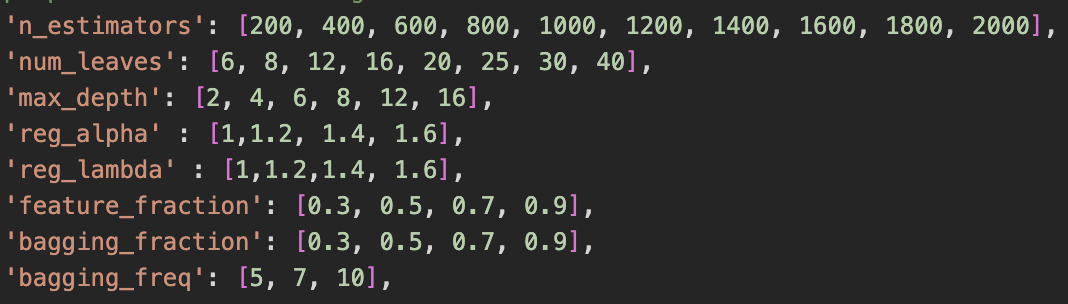
\includegraphics[width=0.9\textwidth]{./plot/ML/RE_RandomSearch.png}
\end{minipage}%
\begin{minipage}{.3\textwidth}
	\centering
	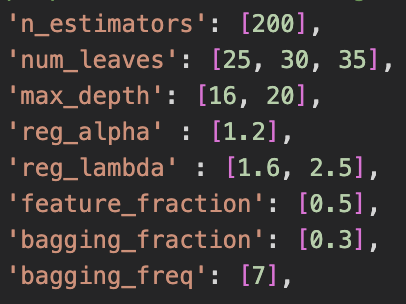
\includegraphics[width=0.9\textwidth]{./plot/ML/RE_GridSearch.png}
\end{minipage}
    \caption{Parameter ranges for Random and Grid Search}
    \label{fig:re_hpsearch}
\end{figure}

\begin{table}[H]
\centering
\begin{tabular}{lrr}\toprule
\textbf{Hyperparameter}                                & \textbf{Random Search} & \textbf{Grid Search} \\\midrule
Number of trees in Random Forest                       & 200                                & 200                              \\
Number of leaves                                       & 25                                 & 30                               \\
Maximum depth of tree                                  & 16                                 & 16                               \\
L1 regularization term on weights                      & 1                                  & 1,2                              \\
L2 regularization term on weights                      & 1,6                                & 1,8                              \\
Fraction of features to be used in each boosting round & 0,5                                & 0,5                              \\
Fraction of data to be used in each boosting round     & 0,3                                & 0,3                              \\
Frequency for bagging                                  & 7                                  & 7                               \\\bottomrule
\end{tabular}
\caption{Best Parameter Settings of Random and Grid Search}
\label{tab:best_rand_grid}
\end{table}

\begin{figure}[H]
	\centering
	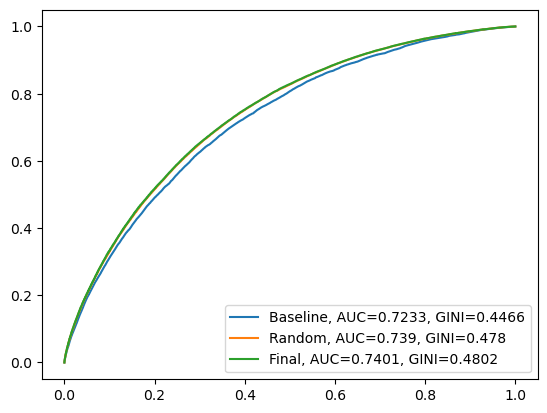
\includegraphics[width=0.65\textwidth]{./plot/ML/ROC_HyperParTuning.png}
    \caption{Performance comparison for Hyperparameter Tuning}
    \label{fig:re_rochp}
\end{figure}

\section{Validation and Comparison}
\label{sec:comp_model}

\subsection{Discriminatory power}
The performance of both models is evaluated using both the test and an out-of-time dataset. To detect potential overfitting, performance metrics for the training sample are also provided. The Gini values are presented in Table \ref{re_ginicomp} and visually represented in Figure \ref{fig:re_roc1} - \ref{fig:re_roc2}. The Random Forest model exhibits a slightly higher performance in the training and test samples, while the logistic regression model shows a slight advantage in the validation sample. Notably, both models demonstrate higher Gini values on the validation sample, indicating no signs of overfitting.

\begin{table}[H]
\centering
\begin{tabular}{lrr}\toprule
\textbf{Sample} & \textbf{Logistic Model} & \textbf{Random Forest} \\\midrule
Training        & 0,4626                  & 0,4708                 \\
Test            & 0,4638                  & 0,4718                 \\
Validation      & 0,4810                  & 0,4734                \\\bottomrule
\end{tabular}
\caption{Comparison of Gini values in training, test and validation sample}
\label{re_ginicomp}
\end{table}

\begin{figure}[H]
\begin{minipage}{.5\textwidth}
	\centering
	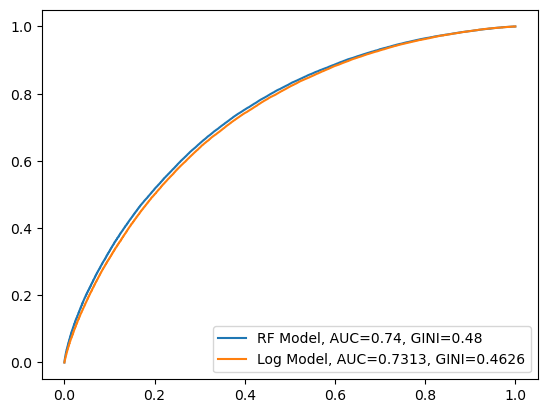
\includegraphics[width=0.9\textwidth]{./plot/ML/ROC_Comp_Train.png}
\end{minipage}%
\begin{minipage}{.5\textwidth}
	\centering
	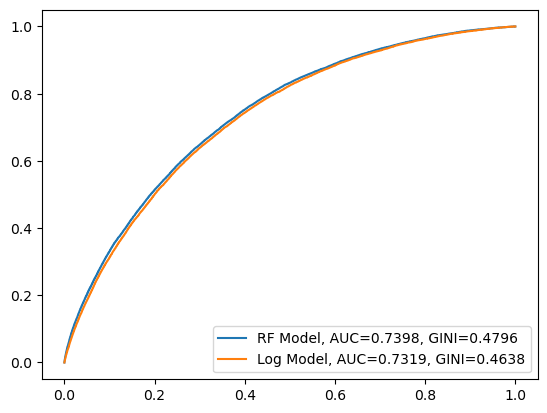
\includegraphics[width=0.9\textwidth]{./plot/ML/ROC_Comp_Test.png}
\end{minipage}
    \caption{AUC comparison in training and test sample}
    \label{fig:re_roc1}
\end{figure}

\begin{figure}[H]
	\centering
	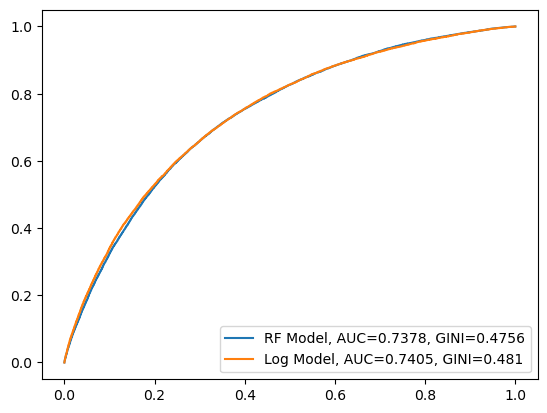
\includegraphics[width=0.65\textwidth]{./plot/ML/ROC_Comp_Validation.png}
    \caption{AUC comparison in Validation sample}
    %\label{fig:re_wholesample}
    \label{fig:re_roc2}
\end{figure}

\subsection{Classification}
To determine an optimal threshold to set a predicted default flag derived from the predicted PD, the F1-score is computed for different values. These values are detailed in Table \ref{tab:re_f1thresh}, leading to the decision to set the threshold at PD > 4\% for both models. The resulting confusion matrices for the training, test and validation sample are visualized in Figure \ref{fig:re_confmatr1} to \ref{fig:re_confmatr3}. On the x-axis, the predicted values are presented, while the y-axis represents true values. Focusing on the most critical cases, where default events are misclassified as non-default (lower left corner), the Random Forest model performs slightly worse in this regard compared to the Logistic Regression model on all samples.

\begin{table}[H]
\centering
\begin{tabular}{ccc}\toprule
								    & \multicolumn{2}{c}{\textbf{F1-Score}}                 \\\midrule
 \textbf{Threshold}                 & \textbf{Logistic Regression} & \textbf{Random Forest} \\
0,005                               & 0,0362                       & 0,0299                 \\
0,010                               & 0,0464                       & 0,0360                 \\
0,015                               & 0,0561                       & 0,0521                 \\
0,020                               & 0,0648                       & 0,0664                 \\
0,025                               & 0,0721                       & 0,0788                 \\
0,030                               & 0,0777                       & 0,0872                 \\
0,035                               & 0,0819                       & 0,0920                 \\
0,040                               & 0,0836                       & 0,0929                 \\
0,045                               & 0,0830                       & 0,0901                 \\
0,050                               & 0,0803                       & 0,0846                 \\
0,055                               & 0,0751                       & 0,0761                 \\
0,060                               & 0,0687                       & 0,0667                 \\
0,065                               & 0,0608                       & 0,0588                 \\
0,070                               & 0,0522                       & 0,0517                 \\
0,075                               & 0,0438                       & 0,0446                 \\
0,080                               & 0,0362                       & 0,0387                 \\
0,085                               & 0,0290                       & 0,0329                 \\
0,090                               & 0,0234                       & 0,0284                 \\
0,095                               & 0,0193                       & 0,0243                \\\bottomrule
\end{tabular}
\caption{F1 score for different threshold values}
\label{tab:re_f1thresh}
\end{table}

\begin{figure}[H]
\begin{minipage}{.5\textwidth}
	\centering
	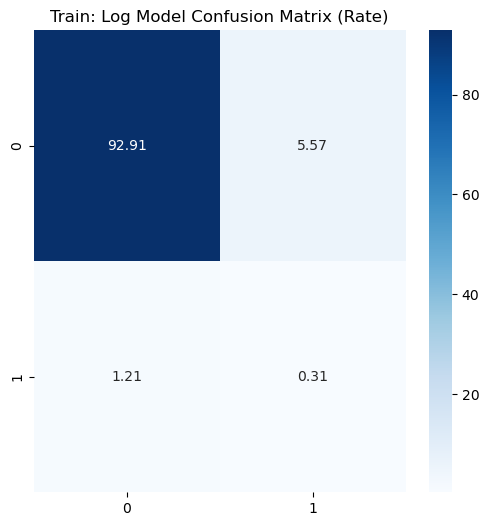
\includegraphics[width=0.9\textwidth]{./plot/ML/ConfMatrix_Train_Log.png}
\end{minipage}%
\begin{minipage}{.5\textwidth}
	\centering
	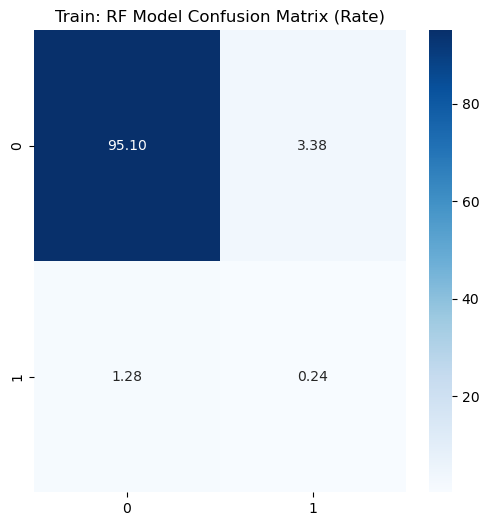
\includegraphics[width=0.9\textwidth]{./plot/ML/ConfMatrix_Train_RF.png}
\end{minipage}
    \caption{Confusionmatrix in training sample}
    \label{fig:re_confmatr1}
\end{figure}
\begin{figure}[H]
\begin{minipage}{.5\textwidth}
	\centering
	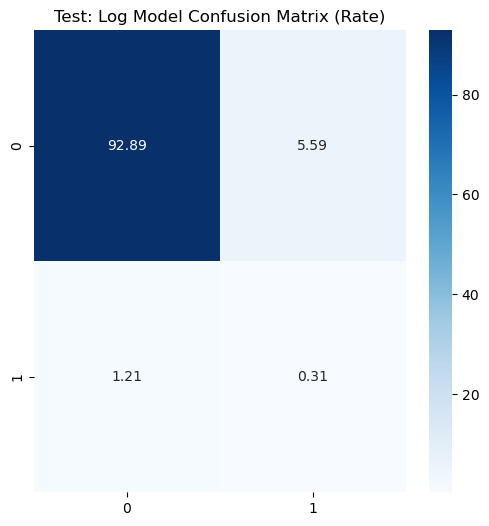
\includegraphics[width=0.9\textwidth]{./plot/ML/ConfMatrix_Test_Log.png}
\end{minipage}%
\begin{minipage}{.5\textwidth}
	\centering
	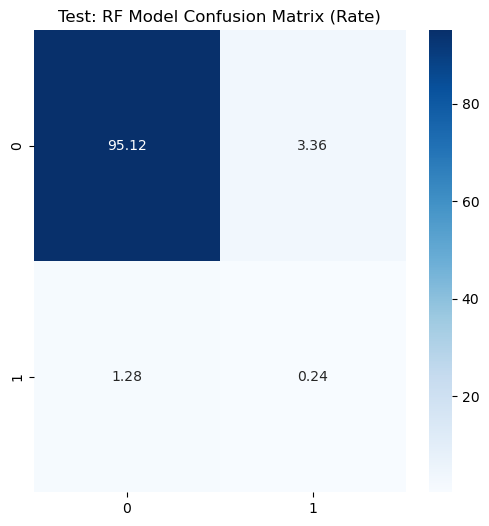
\includegraphics[width=0.9\textwidth]{./plot/ML/ConfMatrix_Test_RF.png}
\end{minipage}
    \caption{Confusionmatrix in test sample}
    %\label{fig:dp_iqr_boxpl}
\end{figure}
\begin{figure}[H]
\begin{minipage}{.5\textwidth}
	\centering
	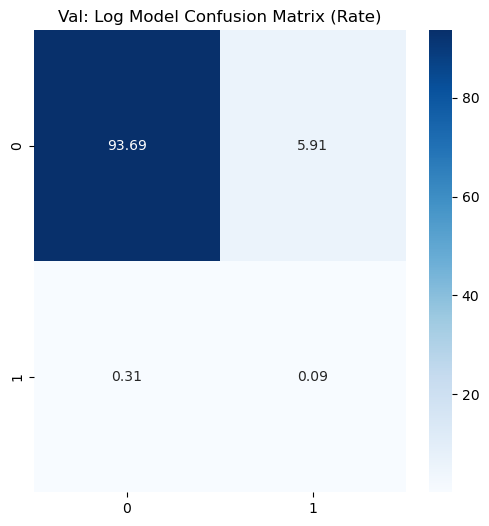
\includegraphics[width=0.9\textwidth]{./plot/ML/ConfMatrix_Val_Log.png}
\end{minipage}%
\begin{minipage}{.5\textwidth}
	\centering
	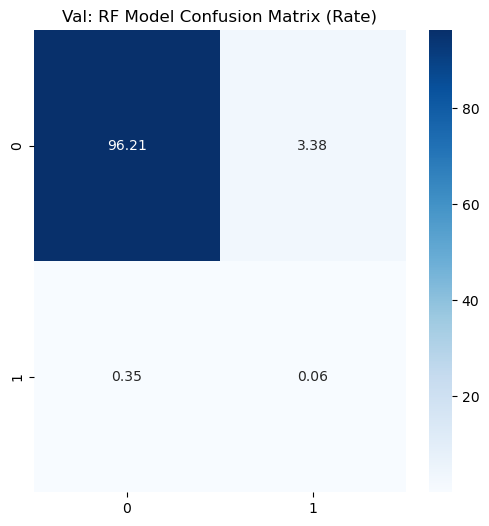
\includegraphics[width=0.9\textwidth]{./plot/ML/ConfMatrix_Val_RF.png}
\end{minipage}
    \caption{Confusionmatrix in validation sample}
    \label{fig:re_confmatr3}
\end{figure}

\subsection{Stability Test}
A stability test for both models was conducted by assessing the Gini coefficient on the test and validation samples for each year, as detailed in Table \ref{tab:re_stab} and illustrated through ROC curves in Figure \ref{fig:re_rocstab}. The left side of the Figure is the logistic model, while the right side showcases the Random Forest model. Both models exhibited their lowest performance in 2019. The logistic model demonstrated its peak discriminatory power in 2018, whereas the Random Forest model excelled in the year 2020. Across the years, both models exhibit a Gini difference of up to 8.4\%, suggesting a moderate level of stability.

\begin{table}[H]
\centering
\begin{tabular}{ccc}\toprule
\textbf{Year} & \textbf{LOG Model} & \textbf{RF Model} \\\midrule
2018          & 0,5202             & 0,5044            \\
2019          & 0,4358             & 0,4440            \\
2020          & 0,4936             & 0,5162            \\
2021          & 0,4810             & 0,4734        	\\\bottomrule   
\end{tabular}
\caption{Stability test over time}
\label{tab:re_stab}
\end{table}

\begin{figure}[H]
\begin{minipage}{.5\textwidth}
	\centering
	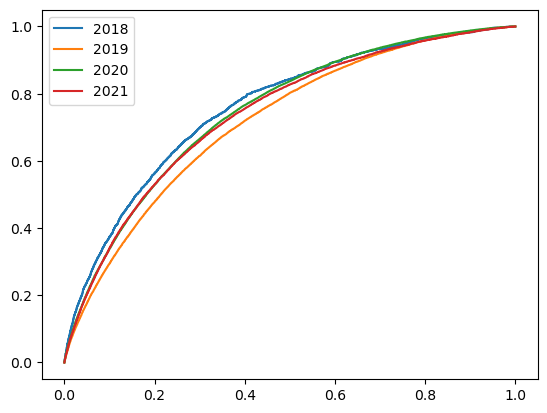
\includegraphics[width=0.9\textwidth]{./Stability_LOG.png}
\end{minipage}%
\begin{minipage}{.5\textwidth}
	\centering
	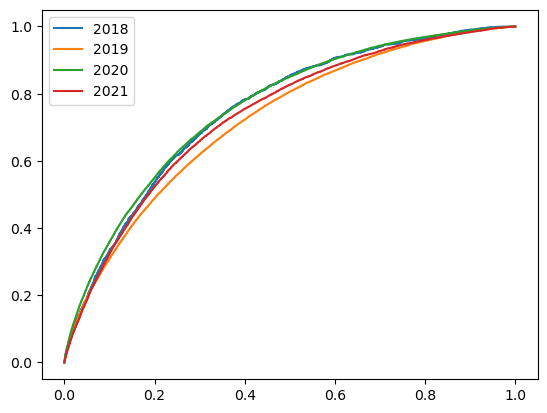
\includegraphics[width=0.9\textwidth]{./Stability_RF.png}
\end{minipage}
    \caption{ROC curve of stability test over time}
    \label{fig:re_rocstab}
\end{figure}

\subsection{Binning Process}
A binning process was executed to provide an overview of the distribution of PDs and default rates. In real-world applications, it is a standard practice to categorize PD values into distinct rating bands, distinguishing between investment and non-investment grades. A straightforward method involves employing fixed ranges for each grade. The specific ranges and the resulting distribution are detailed in Table \ref{tab:re_distrDR} and visually presented in Figure \ref{fig:re_distrDR}. These arbitrary defined ranges already provide a satisfactory distribution, accompanied by a desired upward trend in defaults. The logistic model tends to allocate a greater number of customers with PD values below 0.5\% compared to the Random Forest model. The Random Forest model exhibits a moderate concentration in the range of 1\% to 1.5\%.

\begin{table}[H]
\centering
\begin{tabular}{lrrrrrr}\toprule
\textbf{}        & \multicolumn{2}{c}{\textbf{\# Observation}}                                    & \multicolumn{2}{c}{\textbf{\% Observation}}                                    & \multicolumn{2}{c}{\textbf{\% Default Rate}}                                   \\
\textbf{Range}   & \multicolumn{1}{l}{\textbf{Log}} & \multicolumn{1}{l}{\textbf{RF}} & \multicolumn{1}{l}{\textbf{Log}} & \multicolumn{1}{l}{\textbf{RF}} & \multicolumn{1}{l}{\textbf{Log}} & \multicolumn{1}{l}{\textbf{RF}} \\\midrule
(-inf, 0.001)    & 48.096                                 &                                       & 1\%                                    &                                       & 0,06\%                                 &                                       \\
{[}0.001, 0.005) & 1.665.964                              &                                       & 21\%                                   &                                       & 0,19\%                                 &                                       \\
{[}0.005, 0.01)  & 1.983.432                              & 1.734.463                             & 25\%                                   & 22\%                                  & 0,43\%                                 & 0,17\%                                \\
{[}0.01, 0.015)  & 1.326.997                              & 2.829.949                             & 17\%                                   & 36\%                                  & 0,75\%                                 & 0,48\%                                \\
{[}0.015, 0.02)  & 891.664                                & 1.454.260                             & 11\%                                   & 18\%                                  & 1,09\%                                 & 1,02\%                                \\
{[}0.02, 0.03)   & 1.031.273                              & 1.225.736                             & 13\%                                   & 15\%                                  & 1,58\%                                 & 1,74\%                                \\
{[}0.03, 0.04)   & 493.678                                & 388.029                               & 6\%                                    & 5\%                                   & 2,24\%                                 & 2,65\%                                \\
{[}0.04, inf)    & 470.193                                & 278.860                               & 6\%                                    & 4\%                                   & 3,32\%                                 & 4,06\%        \\\bottomrule                       
\end{tabular}
\caption{Distribution Table of PDs and Default Rates for Logistic Regression and Random Forest Model}
\label{tab:re_distrDR}
\end{table}


\begin{figure}[H]
	\centering
	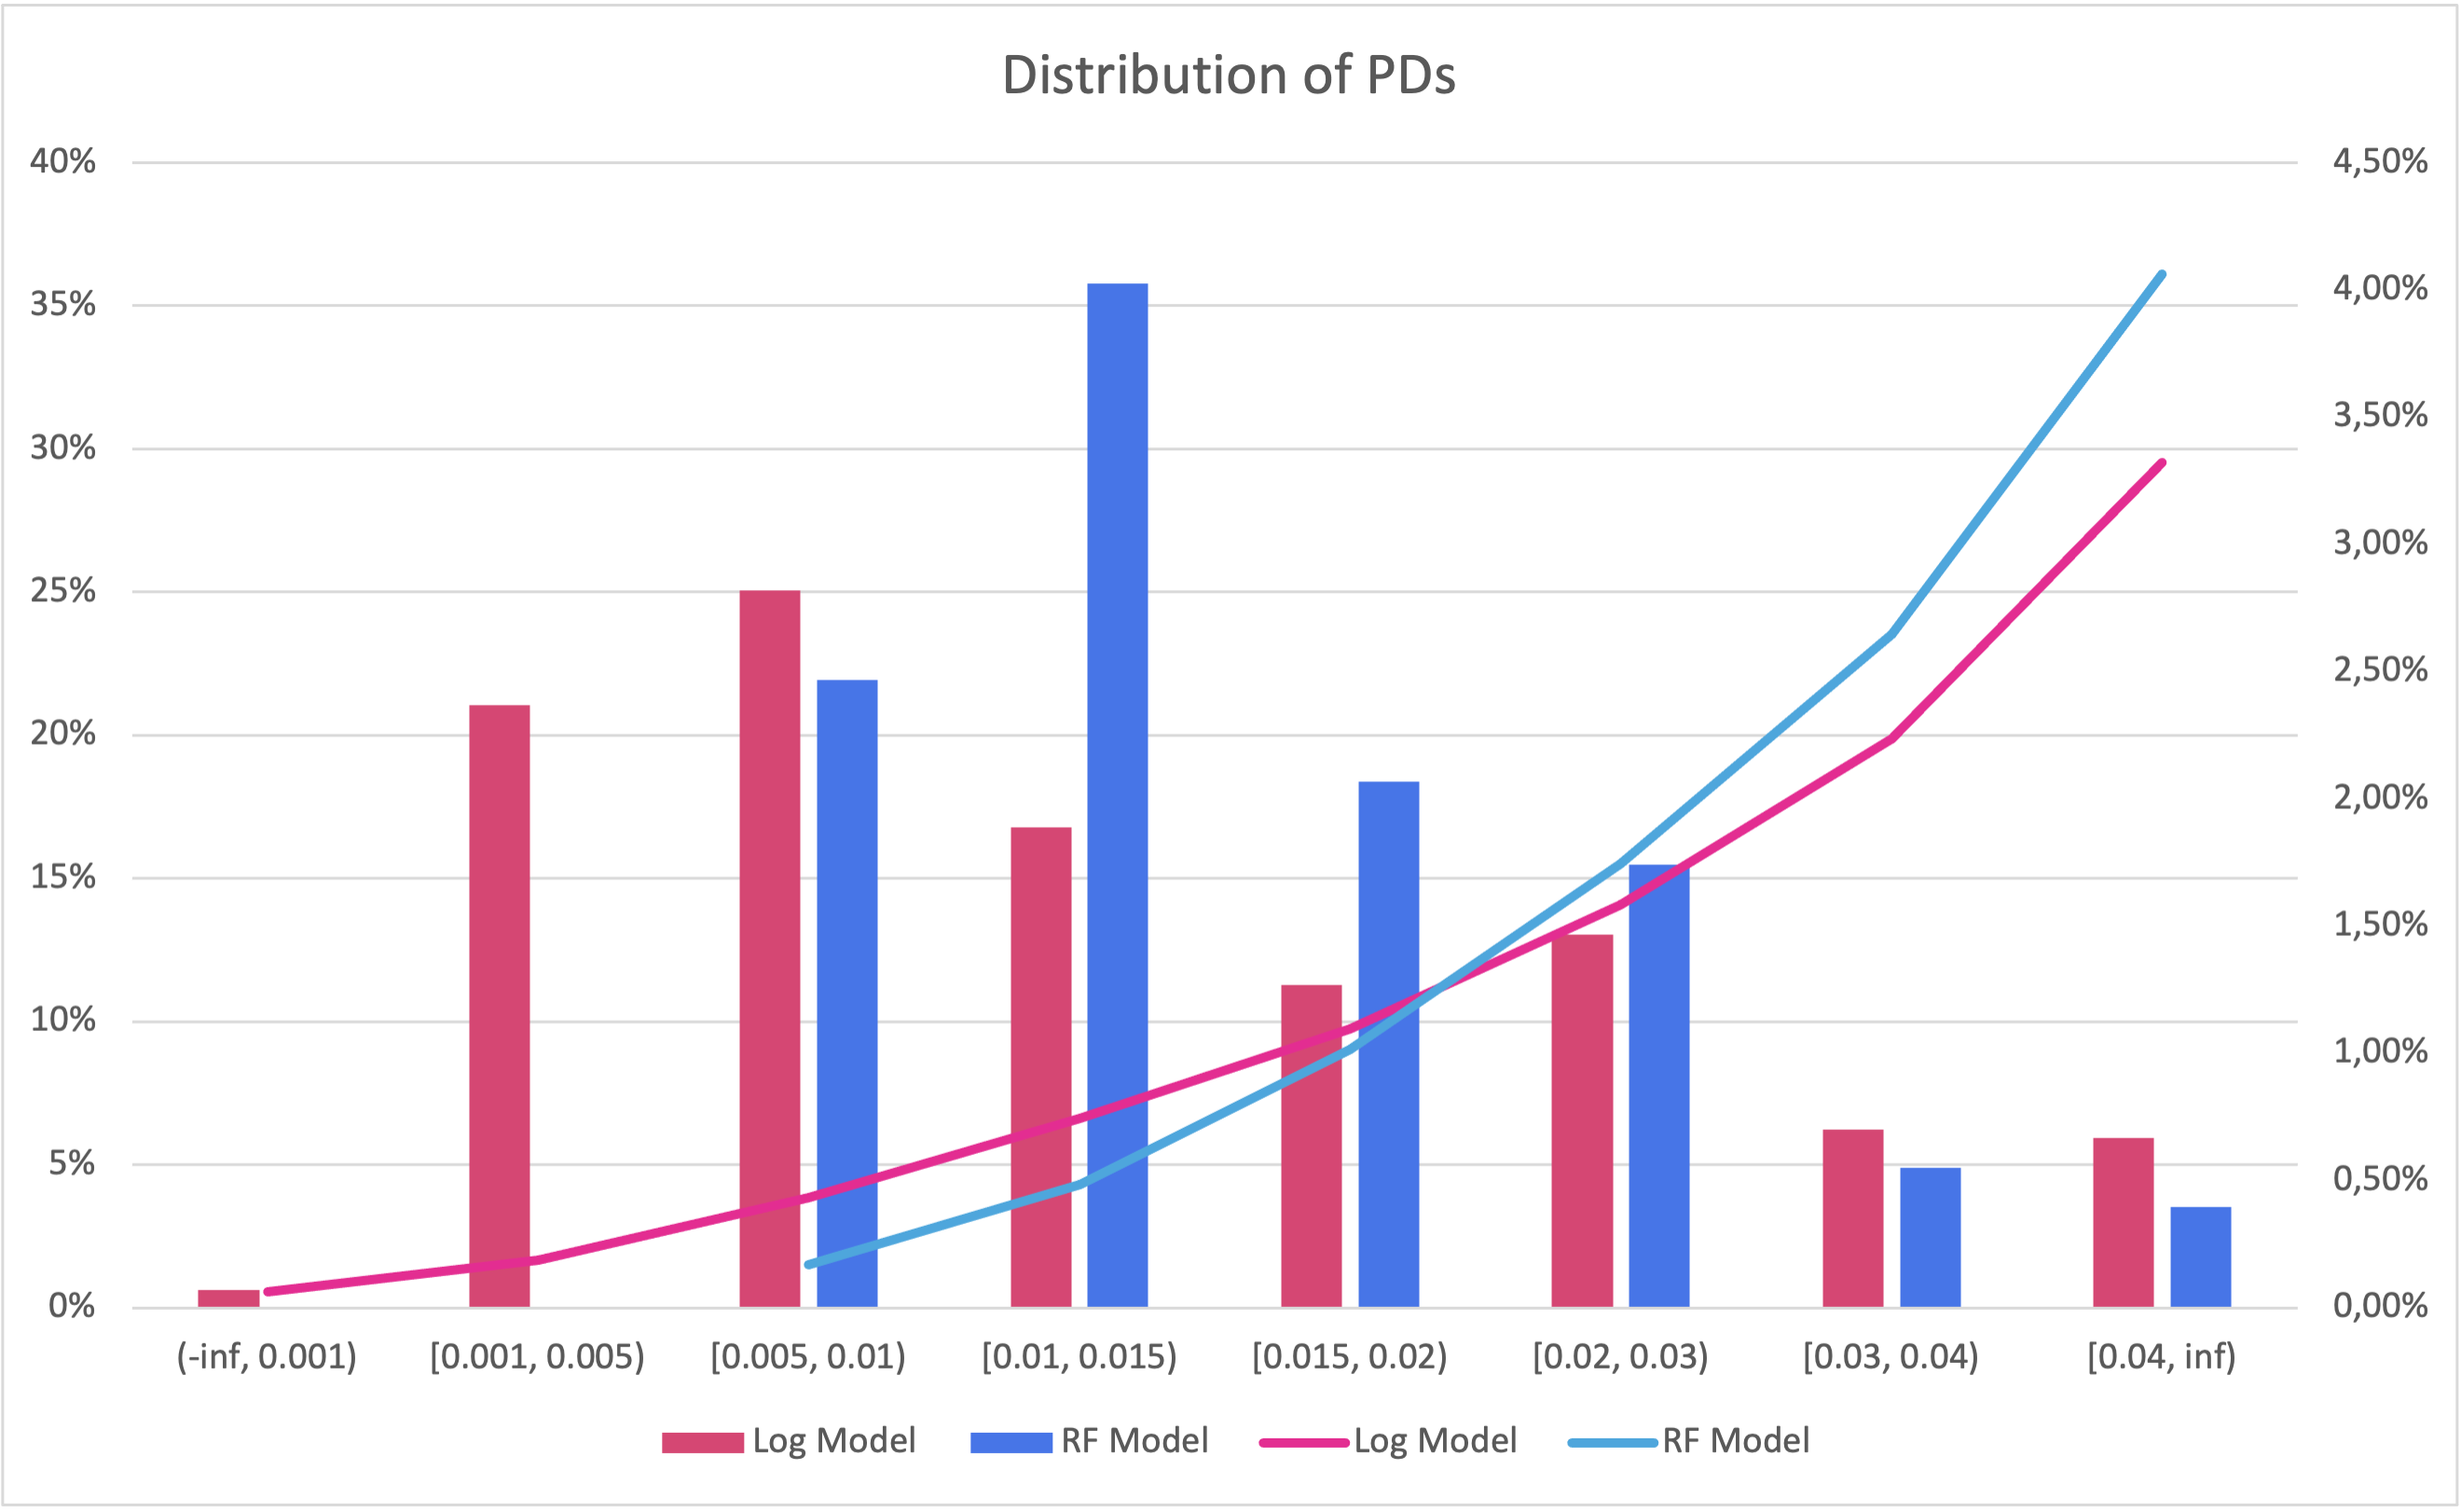
\includegraphics[width=0.9\textwidth]{./plot/ML/RatingGrades.png}
    \caption{Distribution Plot of PDs and Default Rates for Logistic Regression and Random Forest Model}
    %\label{fig:re_wholesample}
    \label{fig:re_distrDR}
\end{figure}

\section{Interpretability}

\subsection{Global Interpretation}
To interpret the Random Forest model, several techniques described in Chapter \ref{sec:interpret} were utilized. Figure \ref{fig:re_featureimp_split} shows the feature importance by split, signifying the frequency with which a variable is employed for a split. Meanwhile, Figure \ref{fig:re_featureimp_gain} depicts feature importance by gain, denoting the information gain derived from the risk factor during a split. Reiterating the findings of the logistic regression model, the most important risk factors in the Random Forest model are \emph{Credit Score} (fico), \emph{UPB}, \emph{CLTV}, \emph{DTI} and \emph{No Borrowers} (cnt\_borr) as well. The \emph{LTV} was removed from the logistic regression model due to its high correlation with the risk factor \emph{CLTV}. 


\begin{figure}[H]
	\centering
	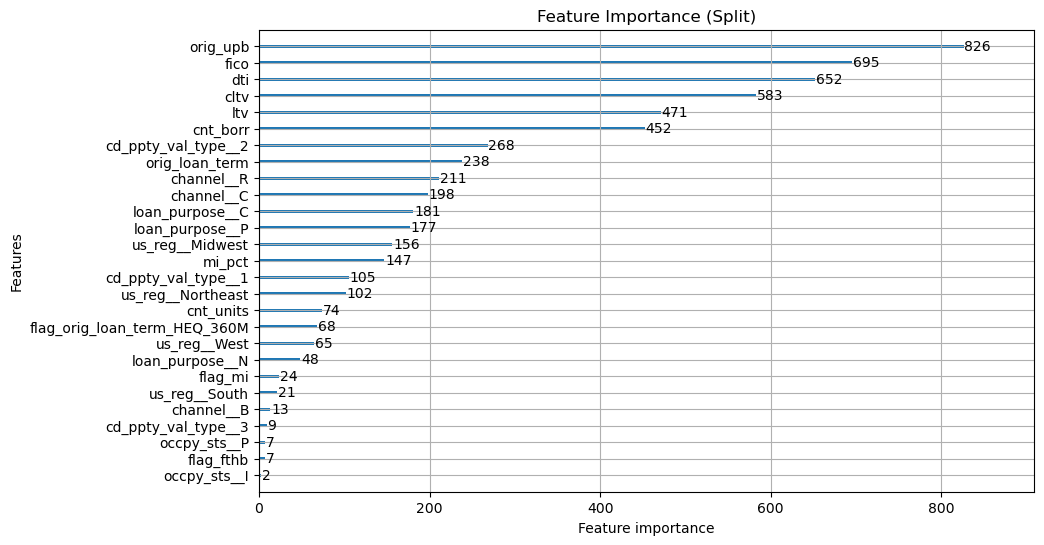
\includegraphics[width=\textwidth]{./plot/ML/FeatureImportanceSplit.png}
    \caption{Feature Importance by Split}
    \label{fig:re_featureimp_split}
\end{figure}

\begin{figure}[H]
	\centering
	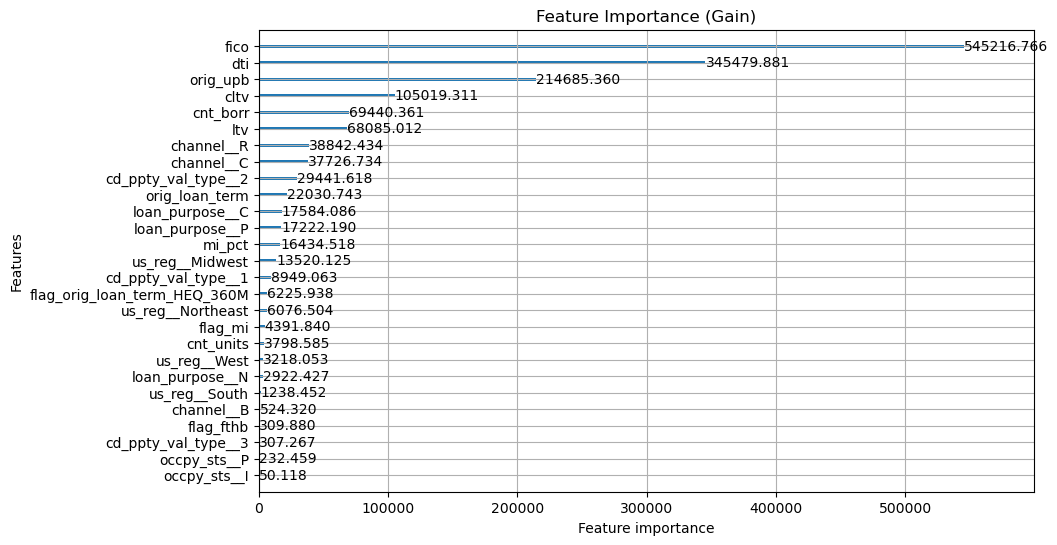
\includegraphics[width=\textwidth]{./plot/ML/FeatureImportanceGain.png}
    \caption{Feature Importance by Gain}
    \label{fig:re_featureimp_gain}
\end{figure}

\subsection{Local Interpretation}
Two particular instances were selected for the Local Interpretable Model-agnostic Explanation (LIME) technique. The first observation received nearly identical PDs of 1.2547\% in both models, while the second observation received vastly different PDs of 59.0619\% in the Logit Model and 2.2576\% in the RF Model. The score composition for the former is displayed in Table \ref{tab:re_PDres} and the LIME results are visible in Figures \ref{fig:re_LIMEres_min} and \ref{fig:re_LIMEres_max}. The green bars indicate the features contributing to predicting the class "non-default" class and the red bars signify the contribution to the "default" class. 

While the high Credit Score mainly influences the low PD in observation 1 for both models, the lower Credit Score, as well as the higher DTI, resulted in a higher PD in the Logit model. Surprisingly, in the RF model, both features contribute to the classification of "non-default", contrasting the result seen in the first observation.

\begin{table}[H]
\centering
\begin{tabular}{l|rrr|rrr}\toprule
\textbf{}                              & \multicolumn{3}{c}{\textbf{Observation 1}}                                                                                                                                                                        & \multicolumn{3}{c}{\textbf{Observation 2}}                                                                                                                                                                       \\
\multicolumn{1}{l|}{\textbf{Variable}} & \multicolumn{1}{c}{\textbf{\begin{tabular}[c]{@{}c@{}}Original\\ Value\end{tabular}}} & \multicolumn{1}{c}{\textbf{\begin{tabular}[c]{@{}c@{}}Scaled\\ Value\end{tabular}}} & \multicolumn{1}{c|}{\textbf{Score}} & \multicolumn{1}{c}{\textbf{\begin{tabular}[c]{@{}c@{}}Original\\ Value\end{tabular}}} & \multicolumn{1}{c}{\textbf{\begin{tabular}[c]{@{}c@{}}Scaled\\ Value\end{tabular}}} & \multicolumn{1}{c}{\textbf{Score}} \\\midrule
\multicolumn{1}{l|}{Intercept}         &                                                                                       &                                                                                     & \multicolumn{1}{r|}{-4,5457}        &                                                                                       &                                                                                     & -4,5457                            \\
\multicolumn{1}{l|}{Credit Score}      & 691                                                                                   & -           1,4100                                                                  & \multicolumn{1}{r|}{0,7642}         & 309                                                                                   & -        10,1100                                                                    & 5,4796                             \\
\multicolumn{1}{l|}{DTI}               & 29,99                                                                                 & -           0,4421                                                                  & \multicolumn{1}{r|}{-0,1802}        & 40,01                                                                                 & 0,5910                                                                              & 0,2409                             \\
\multicolumn{1}{l|}{CLTV}              & 73,00                                                                                 & -           0,0359                                                                  & \multicolumn{1}{r|}{-0,0094}        & 30,00                                                                                 & -           2,5257                                                                  & -0,6600                            \\
\multicolumn{1}{l|}{No Borrowers}      & 2                                                                                     & 0,9969                                                                              & \multicolumn{1}{r|}{-0,2476}        & 1                                                                                     & -           0,9326                                                                  & 0,2317                             \\
\multicolumn{1}{l|}{UPB}               & 200.000                                                                               & -           0,4313                                                                  & \multicolumn{1}{r|}{-0,1469}        & 110.000                                                                               & -           1,1133                                                                  & -0,3793                            \\
\multicolumn{1}{l|}{Model Score}       & \multicolumn{3}{c|}{-4,3656}                                                                                                                                                                                      & \multicolumn{3}{c}{0,3672}                                                                                                                                                                                       \\
\multicolumn{1}{l|}{PD}                & \multicolumn{3}{c|}{1,25\%}                                                                                                                                                                                       & \multicolumn{3}{c}{59,08\%} \\\bottomrule                                                                                                                                                                                     
\end{tabular}
\caption{PD Result of Logistic Regression model}
\label{tab:re_PDres}
\end{table}

\begin{figure}[H]
	\centering
	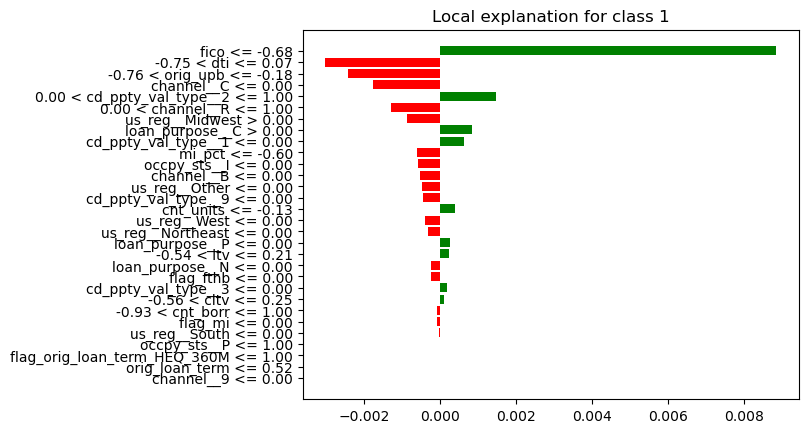
\includegraphics[width=0.9\textwidth]{./plot/ML/LIME_minDiff.png}
    \caption{LIME Result of Random Forest, minimum difference in PD}
    \label{fig:re_LIMEres_min}
\end{figure}

\begin{figure}[H]
	\centering
	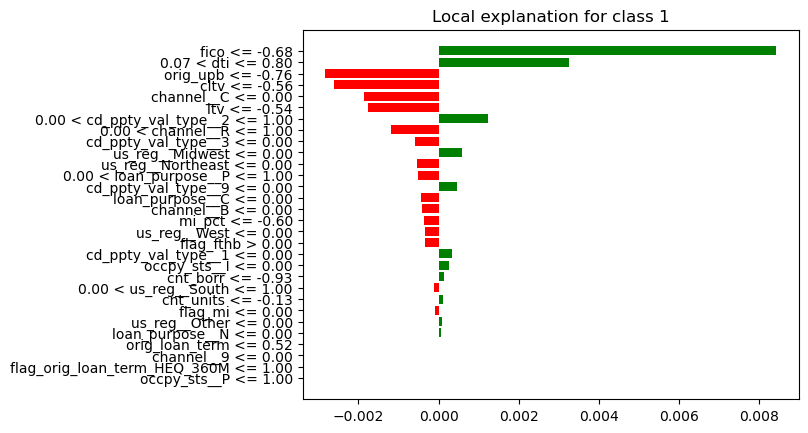
\includegraphics[width=0.9\textwidth]{./plot/ML/LIME_maxDiff.png}
    \caption{LIME Result of Random Forest, maximum difference in PD}
    \label{fig:re_LIMEres_max}
\end{figure}

\subsection{Individual Decision Trees, PDP and ICE plots}
Two individual decision trees from the Random Forest model are presented in Figure \ref{fig:re_indtree1} and \ref{fig:re_indtree2}. Analyzing the split conditions, they reaffirm the importance of \emph{Credit Score}, \emph{UPB}, \emph{DTI} and \emph{LTV} as primary variables. To assess their influence, Partial Dependence plots of these four features, along with \emph{Prop Val Method = Full Appraisal} and \emph{Loan Purpose = Refinance - Cash Out} are showcased in Figure \ref{fig:pdp_1} to \ref{fig:pdp_2}. All plots are in Appendix \ref{sec:PDP_all}. The observed trends align with the economic rationale: increasing Credit Score corresponds to decreasing PD, while rising UPB, DTI and CLTV are associated with higher PD. Both categorical variables indicate a higher PD if the condition is fulfilled. Individual Conditional Expectation (ICE) plots were generated to further analyze the impact of the four most crucial features. Figure \ref{fig:ice_1} to \ref{fig:ice_2} provide a granular analysis of each feature's influence on individual predictions. The findings from these ICE plots also align with the anticipated relationship between the respective risk factor and the PD estimation.

\begin{figure}[H]
	\centering
	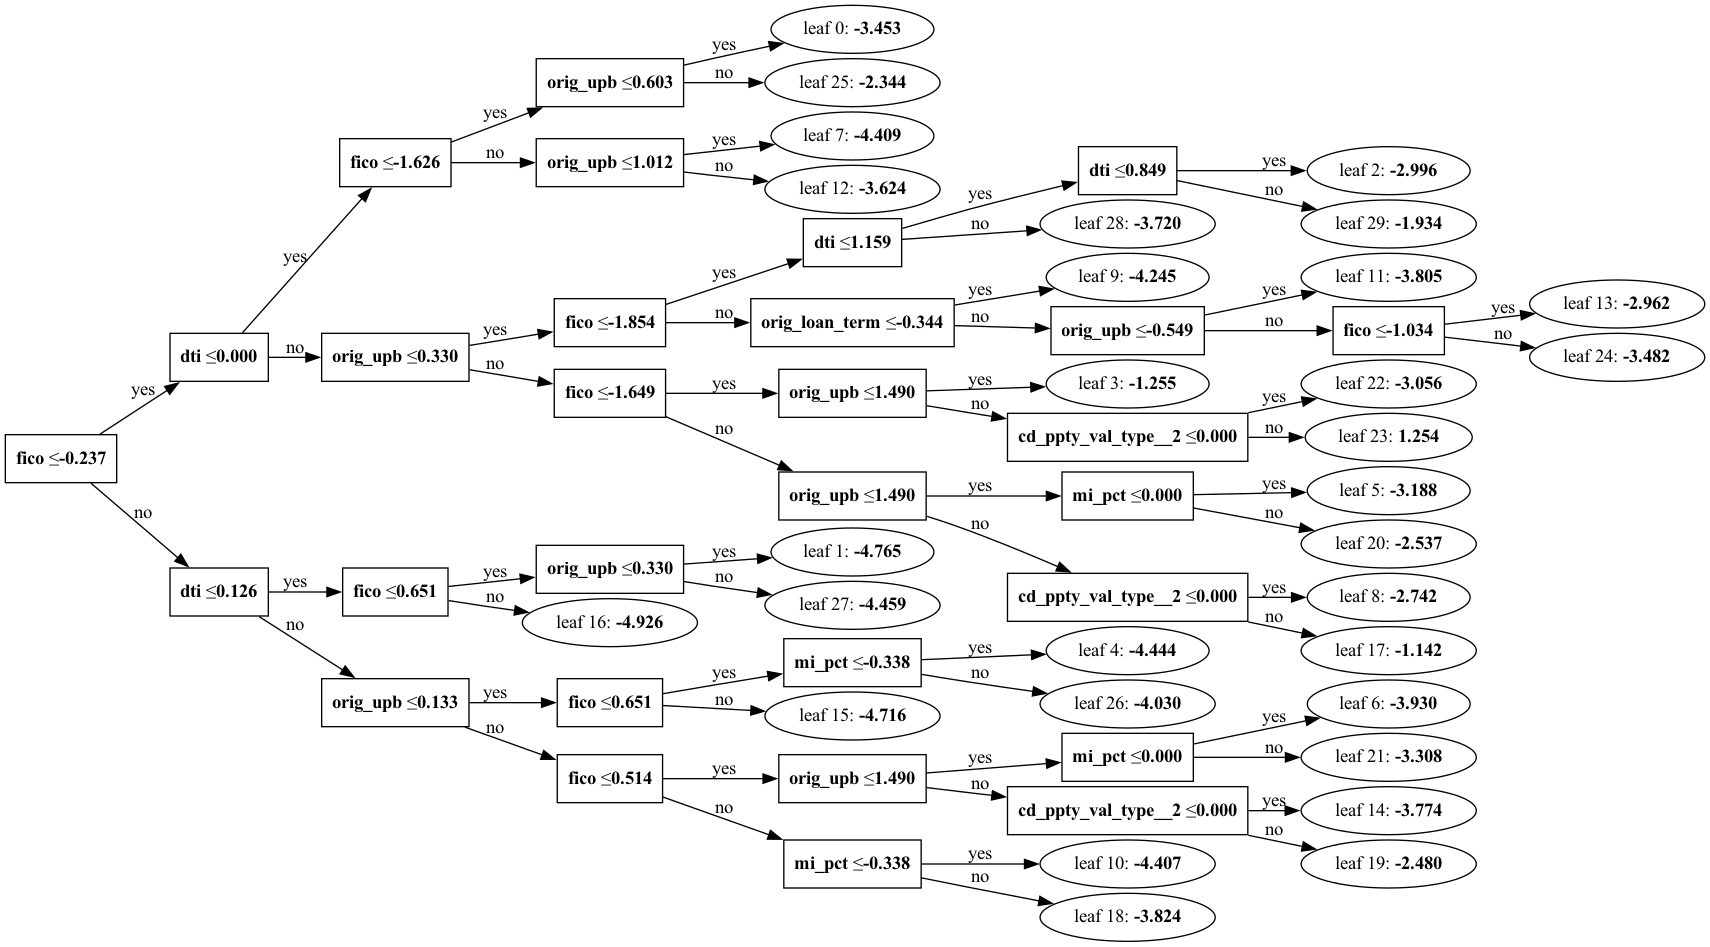
\includegraphics[width=0.9\textwidth]{./plot/ML/IndDecTree1.png}
    \caption{Individual Decision Tree 1 of Random Forest}
    %\label{fig:re_wholesample}
    \label{fig:re_indtree1}
\end{figure}

\begin{figure}[H]
	\centering
	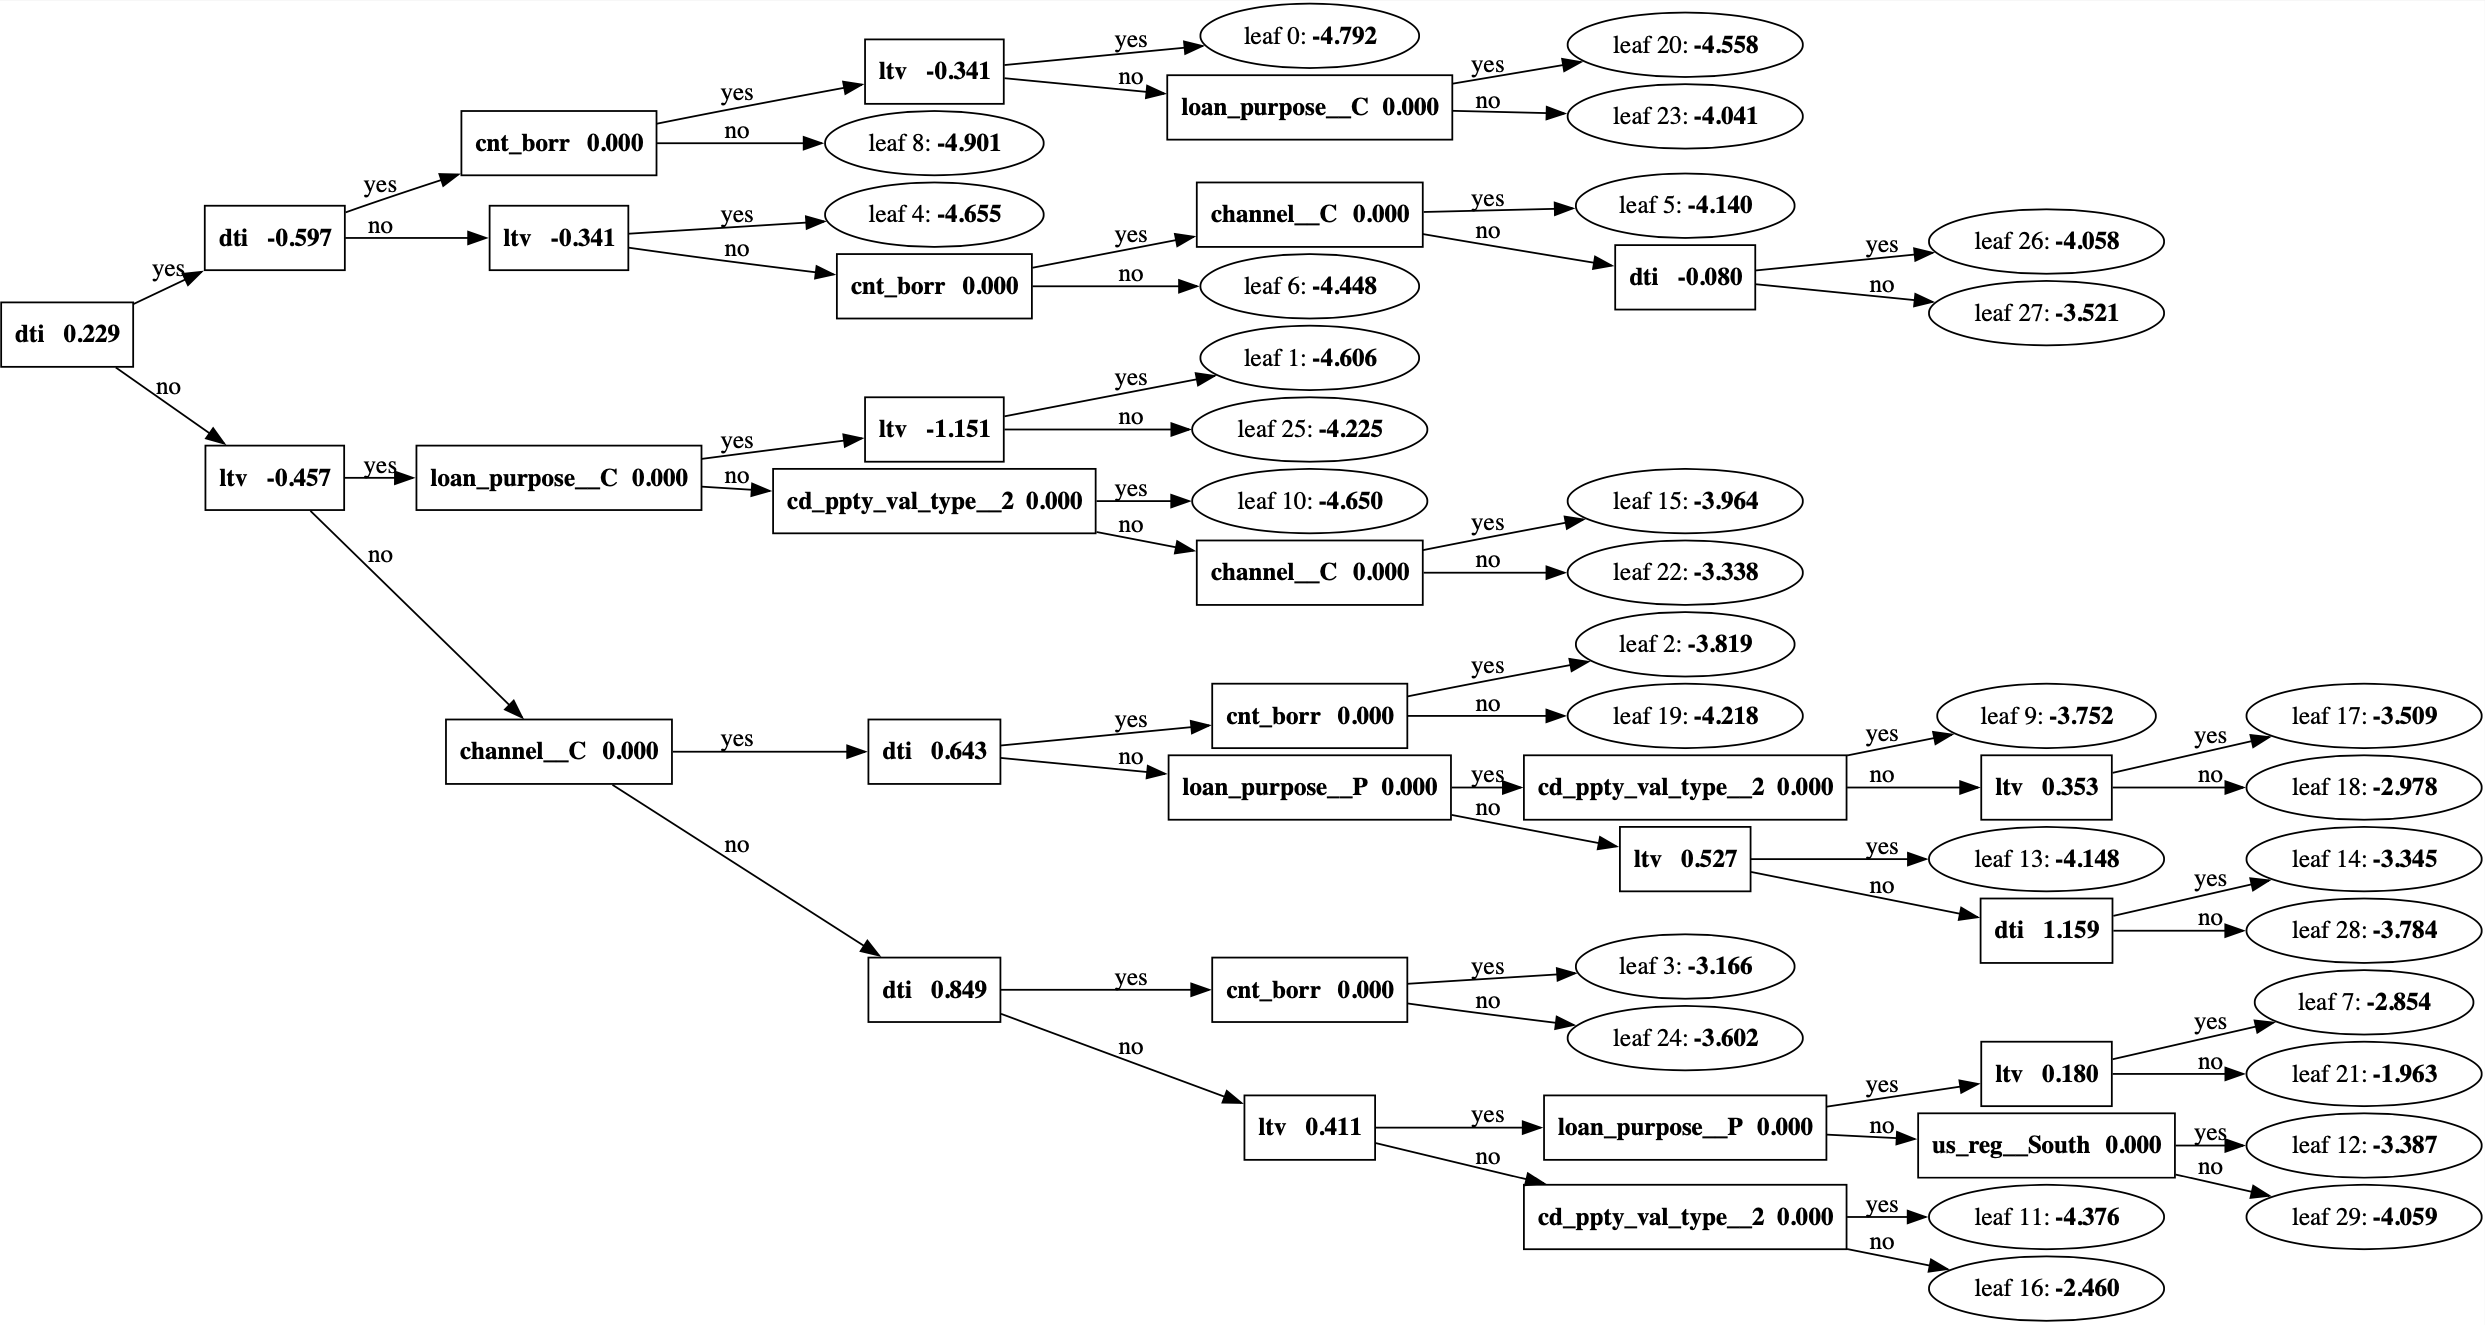
\includegraphics[width=0.9\textwidth]{./plot/ML/IndDecTree2.png}
    \caption{Individual Decision Tree 2 of Random Forest}
    %\label{fig:re_wholesample}
    \label{fig:re_indtree2}
\end{figure}

\begin{figure}[H]
\begin{minipage}{.5\textwidth}
	\centering
	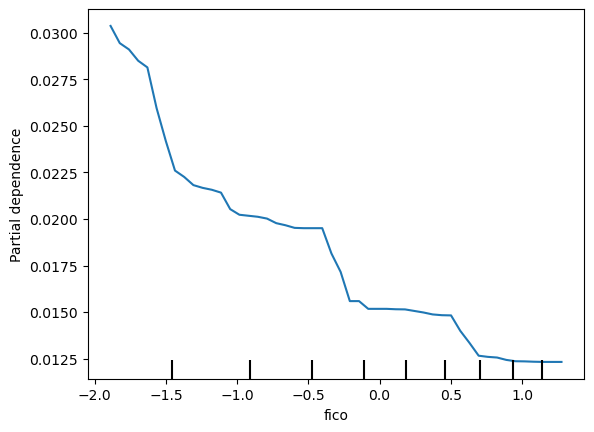
\includegraphics[width=0.9\textwidth]{./plot/ML/PDP_fico.png}
\end{minipage}%
\begin{minipage}{.5\textwidth}
	\centering
	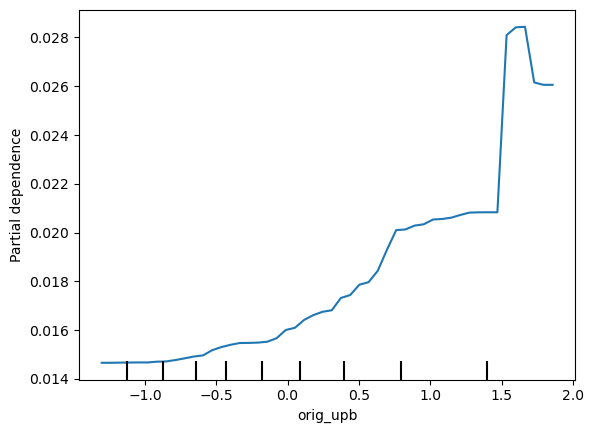
\includegraphics[width=0.9\textwidth]{./plot/ML/PDP_orig_upb.png}
\end{minipage}
    \caption{Partial Dependence Plots for Credit score and UPB}
    \label{fig:pdp_1}
\end{figure}

\begin{figure}[H]
\begin{minipage}{.5\textwidth}
	\centering
	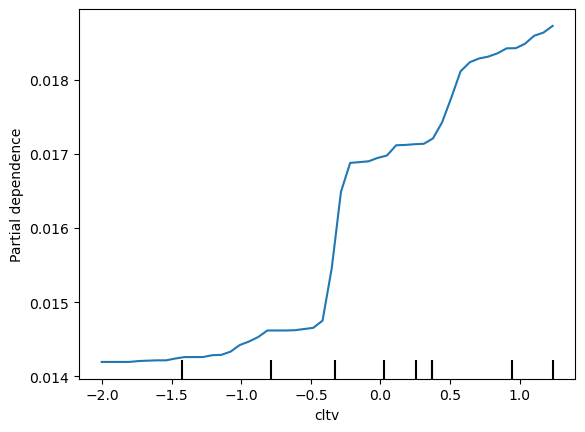
\includegraphics[width=0.9\textwidth]{./plot/ML/PDP_cltv.png}
\end{minipage}%
\begin{minipage}{.5\textwidth}
	\centering
	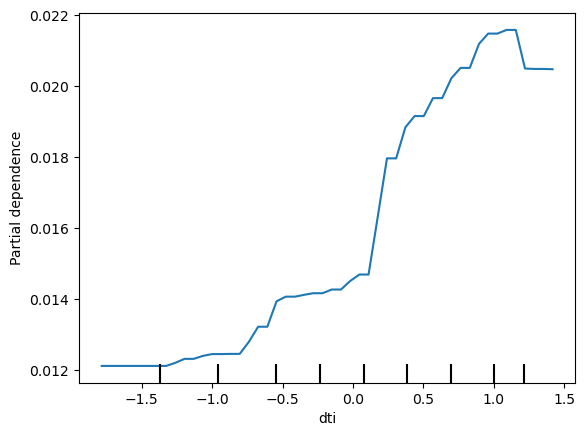
\includegraphics[width=0.9\textwidth]{./plot/ML/PDP_dti.png}
\end{minipage}
    \caption{Partial Dependence Plots for CLTV and DTI}
    %\label{fig:dp_iqr_boxpl}
\end{figure}

\begin{figure}[H]
\begin{minipage}{.5\textwidth}
	\centering
	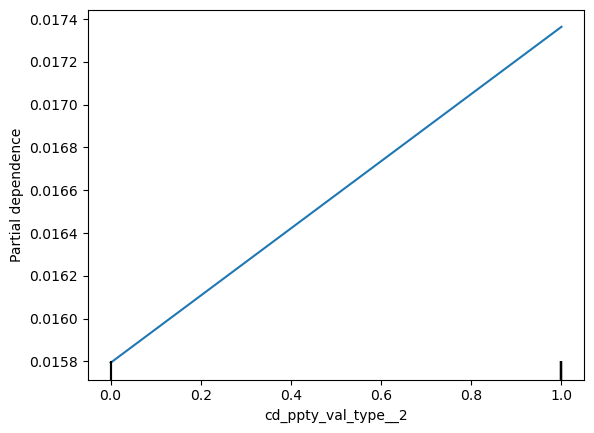
\includegraphics[width=0.9\textwidth]{./plot/ML/PDP_cd_ppty_val_type__2.png}
\end{minipage}%
\begin{minipage}{.5\textwidth}
	\centering
	\includegraphics[width=0.9\textwidth]{./plot/ML/PDP_loan_purpose__C.png}
\end{minipage}
    \caption{Partial Dependence Plots for Prop Val Method = Full Appraisal and Loan Purpose = Refinance - Cash Out}
    \label{fig:pdp_2}
\end{figure}

\begin{figure}[H]
\begin{minipage}{.5\textwidth}
	\centering
	\includegraphics[width=0.9\textwidth]{./plot/ML/ICE_fico.png}
\end{minipage}%
\begin{minipage}{.5\textwidth}
	\centering
	\includegraphics[width=0.9\textwidth]{./plot/ML/ICE_orig_upb.png}
\end{minipage}
    \caption{Individual Conditional Expectation Plots for Credit Score and UPB}
    \label{fig:ice_1}
\end{figure}

\begin{figure}[H]
\begin{minipage}{.5\textwidth}
	\centering
	\includegraphics[width=0.9\textwidth]{./plot/ML/ICE_cltv.png}
\end{minipage}%
\begin{minipage}{.5\textwidth}
	\centering
	\includegraphics[width=0.9\textwidth]{./plot/ML/ICE_dti.png}
\end{minipage}
    \caption{Individual Conditional Expectation Plots for CLTV and DTI}
    \label{fig:ice_2}
\end{figure}
